\documentclass[12pt]{report}

\usepackage{layouts}
\usepackage{morefloats}
\usepackage{epsfig,amsfonts,amsmath,amstext,amssymb,latexsym}
\usepackage{theorem,algorithmic,algorithm,graphicx,pxfonts,txfonts}
%\usepackage{fancyheadings}
\usepackage{fancyhdr}
\usepackage{boxedminipage,mathrsfs,verbatim}
\usepackage{float,calc}
\usepackage{subfigure}
\usepackage[draft]{varioref}
\vrefwarning
\usepackage{color}
\usepackage{listings} 
\usepackage{textcomp,pgfpict2e,tikz}



\usepackage[utf8]{inputenc}
\usepackage[english]{babel}
\usepackage{float}
\setcounter{secnumdepth}{3}



\bibliographystyle{plain}

\lstset{ %configuring the display of scilab codes
			tabsize=4,
			language=scilab,
			aboveskip={1\baselineskip},
			showstringspaces=false,
			breaklines=true,
			showspaces=false,
			numbers=left,
			numberstyle=\tiny,
			commentstyle=\scriptsize}
\usetikzlibrary{shapes,arrows}
\tikzstyle{block} = [draw, fill=white!20, rectangle, 
    minimum height=3em, minimum width=6em]
\tikzstyle{sum} = [draw, fill=white!20, circle, node distance=1cm]
\tikzstyle{input} = [coordinate]
\tikzstyle{output} = [coordinate]
\tikzstyle{pinstyle} = [pin edge={to-,thin,black}]
\tikzstyle{branch} = [circle,inner sep=0pt,minimum size=1mm,fill=black,draw=black]

% code environment

{\theorembodyfont{\rmfamily} \newtheorem{codemass}{Scilab Code}[chapter]}
\newenvironment{code}%
{\begin{codemass}}{\hrule \end{codemass}}

% create listing for code

\newcommand\ccaption[1]
     {\addcontentsline{cod}{section}{\protect\numberline {\thecodemass}#1}}
\makeatletter \newcommand\listofcode
     {\chapter*{List of Scilab Code\markboth%
                        {\bf List of Scilab Code}{}}%
\renewcommand*\l@section{\@dottedtocline{1}{1.5em}{3em}}%
\addcontentsline{toc}{chapter}{\protect\numberline{List of Scilab\ Code}}
\@starttoc{cod}}
\newcommand\l@matlab[3]
     {#1 \par\noindent#2, #3 \par} 
\renewcommand\@pnumwidth{2.1em}
\makeatother

\title{Documentation 
for \\ Single Board Heater System}
\author{Rakhi R\\Rupak Rokade \\ Inderpreet Arora \\ Kannan M. Moudgalya \\ Kaushik Venkata Belusonti\vspace{1in}}


\date{
\begin{figure}[h]
\centering

\includegraphics[width=0.3\linewidth]{iitblogo.pdf}
\end{figure}IIT Bombay \\\today}

\begin{document}


%\begin{figure}
%\begin{center}
%\begin{tikzpicture}[auto,node distance=2cm]
%\node[input](input){};
%\node[block,right of=input](tcbyrc){$\gamma \frac{T_c(z)}{R_c(z)}$};
%\draw[->](input)--node{$r$}(tcbyrc);
%\node[sum,right of=tcbyrc,node distance=2cm](sum1){};
%\draw[->](tcbyrc)--node{}(sum1);
%\node[block,right of=sum1](plant){$G=z^{-k}\frac{B(z)}{A(z)}$};
%\draw[->](sum1)--node{$u$}(plant);
%\node[output,right of=plant](output){};
%\draw[->](plant)--node[name=y]{$y$}(output);
%\node[block,below of=plant](scbyrc){$\frac{S_c}{R_c}$};
%\draw[->](y)|-node{}(scbyrc);
%\draw[->](scbyrc)-|node[pos=0.99]{$-$}(sum1);
%\end{tikzpicture}
%\end{center}
%\caption{2-DOF pole placement controller}
%\label{2dofppc}
%\end{figure}


\maketitle
\tableofcontents
\listofcode
\chapter{Block diagram explanation of Single Board Heater System}
\begin{figure}
\centering
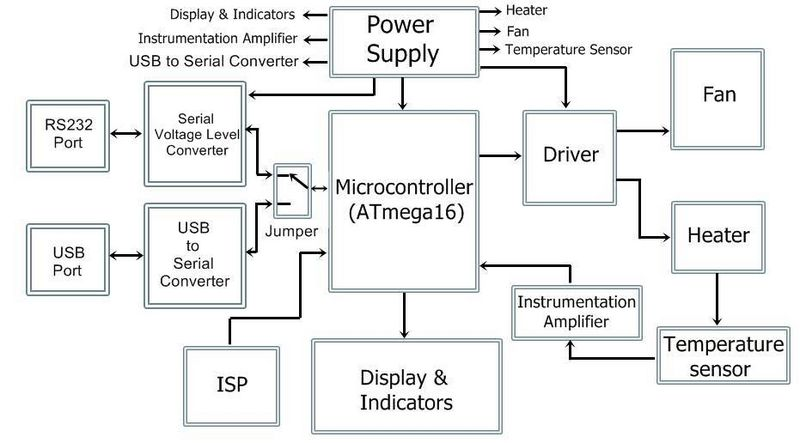
\includegraphics[width=\linewidth]{blkdiag.jpg}
\caption{Block Diagram}
\label{blkdig}
\end{figure}
Figure\ref{blkdig} shows the block diagram of \textquoteleft Single Board Heater System\textquoteright. Microcontroller ATmega16 is used and is the heart of the setup. Two serial communication ports namely RS232 and USB can be used to connect the setup to a computer. A particular port can be selected by setting the jumper to its appropriate place. The communication between PC and setup takes place via a serial to TTL interface. The microcontroller can be programmed with the help of an In-system programmer port(ISP) available on the board. The \textmu C operates the Heater and Fan with the help of separate drivers. The driver comprises of a power MOSFET. A temperature sensor is used to sense the temperature and fed to the \textmu C through an Instrumentation amplifier. Some required parameter values are displayed along with some LED indications.
\section{Microcontroller}
Some salient features of ATmega16 are listed below
\begin{enumerate}
\item 32 x 8 general purpose registers.
\item 16K Bytes of In-System Self-Programmable flash memory
\item 512 Bytes of EEPROM
\item 1K Bytes of internal Static RAM (SRAM)
\item Two 8-bit Timer/Counters
\item One 16-bit Timer/Counter
\item Four PWM channels
\item 8-channel,10-bit ADC
\item Programmable Serial USART
\item Up to 16 MIPS throughput at 16 MHz
\end{enumerate}
Microcontroller plays a very important role. It controls every single hardware present on the board, directly or indirectly. It executes various tasks like, setting up communication between PC and the equipment, controlling the amount of current passing through the heater coil, controlling the fan speed, reading the temperature, displaying some relevant parameter values and various other necessary operations.
\subsection{PWM for heat and speed control}
The Single Board Heater System has a Heater coil and a Fan. The heater assembly consists of an iron plate placed at a distance of about 3.5mm from a nichrome coil. When current passes through the coil it gets heated and in turn raises the temperature of the iron plate. We are interested to alter the heat generated by the coil and also the speed at which the fan is operated.
There are many ways to control the amount of power delivered to the Fan and Heater. We are using the PWM technique.
PWM or pulse width modulation is a process in which the duty cycle of the square wave is modulated.
\begin{align}
      \text{Duty cycle} = \frac{T_{ON}}{T}
\end{align}
Where $T_{ON}$ is the ON time of the wave and  T is the total time period of the wave. Power delivered to the load is proportional to T- ON time of the signal. This is used to control the current flowing through the heating element and also speed of the fan.
\begin{figure}
\centering
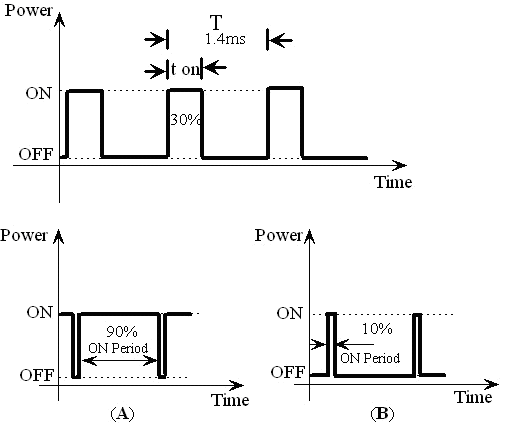
\includegraphics[width=0.5\linewidth]{pwm}
\caption{Pulse Width Modulation (A): On time is $90\%$ of the total time period,    (B): ON time is $10\%$ of total time period}
\end{figure} 
An internal timer of the microcontroller is used to generate a square wave. The ON time of the square wave depends on a count value. Hence, by varying this count value one can vary the width of the waveform. Therefore, by using this technique, PWM waveform is generated at the appropriate pin of the microcontroller. This generated PWM waveform is used to control the power delivered to the load (Fan and Heater). A MOSFET is used to switch at the PWM frequency which indirectly controls the power delivered to the load. A separate MOSFET is used for the two loads. The timer is operated at 244Hz.
\subsection{Analog to Digital conversion}
As explained earlier, the heat generated by the heater coil is passed to the iron plate through convection. We would now want to measure the temperature of this plate. For this purpose a temperature sensor AD590 is used.
Some of the salient features of AD590 include
\begin{enumerate}
\item Linear current output: 1\textmu A/K
\item Wide range: -55\textcelsius to +150\textcelsius
\item Sensor isolation from case
\item Low cost
\end{enumerate}
The output of AD590 is then fed to the microcontroller through an Instrumentation amplifier. The signal so obtained would be in analog form. It has to be converted in to digital form to make it understandable for the microcontroller. An ADC would be an obvious solution. ATmega16 features an 8-channel , 10 bit successive approximation ADC with 0-Vcc(0 to Vcc) input voltage range. An interrupt is generated on completion of analog to digital conversion. Here, ADC is initialize to have 206 $\mu$ sec of conversion time . Digital data so obtained is sent to computer via serial port as well as for further processing for on board display.
\section{Instrumentation amplifier}
Whenever there is a temperature measurement task at hand, instrumentation amplifiers are often used. A typical three Op-Amp Instrumentation amplifier is shown in the figure\ref{instramp}.
\begin{figure}
\centering
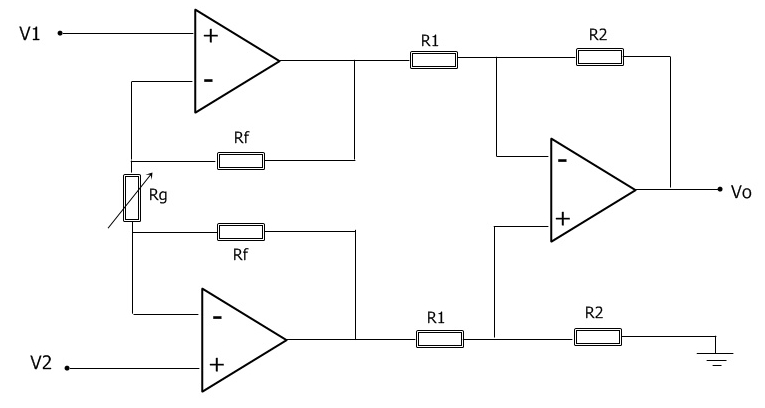
\includegraphics[width=0.6\linewidth]{Inst_Amp}
\caption{3 Op-Amp Instrumentation Amplifier}
\label{instramp}
\end{figure}
The instrumentation amplifiers (IA)have the advantage of very low DC offsets, high input impedance, very high Common mode rejection ratio (CMRR) etc. They are mostly prefered where the sensor is located at a remote place, susceptible to signal attenuation. The IA's have a very high input impedance and hence dose not loads the input signal source. IC LM348 is used to construct a 3 Op-Amp IA. IC LM348 contains a set of four Op-Amps. Gain of the amplifier is given by equation \ref{ia}
\begin{align}
\frac{V_o}{V_2-V_1}=\left\{1+\frac{2R_f}{R_g}\right\}\frac{R_2}{R_1}
\label{ia}
\end{align} 
The value of $R_g$ is kept variable to change the overall gain of the amplifier.
The signal generated by AD590 is in \textmu A/\textdegree K.  It is converted to mV/\textdegree K by taking it across a 1K\textohm  resistor. The  \textdegree K to\textdegree C conversion is done by subtracting 237 from the \textdegree K result. One input of the IA is fed with the mV/\textdegree K reading and the other with 273mV. The resulting output is now in mV/\textdegree C. The output of the IA is fed to microcontroller for further processing.
\section{Communication}
The set up has the facility to use either USB or RS232 for communication between set up and computer. A jumper is been provided to switch between USB and RS232.
\begin{figure}
\centering
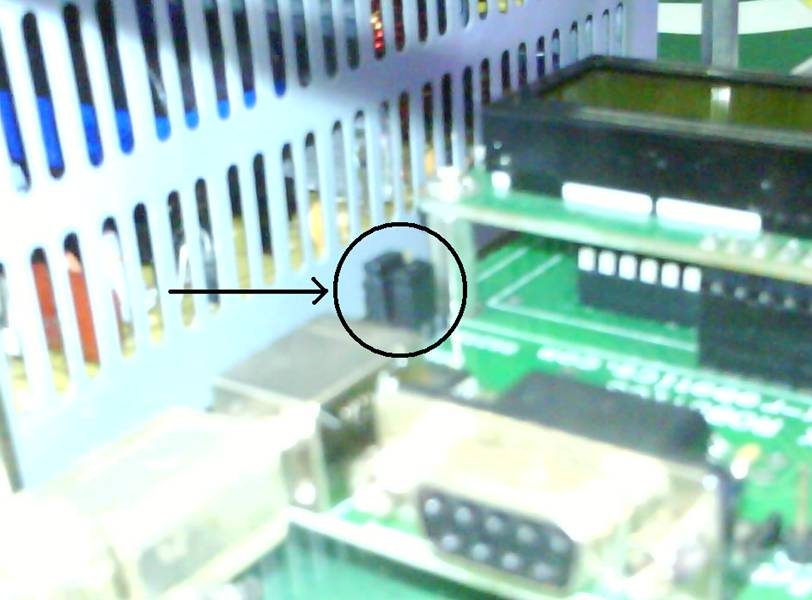
\includegraphics[width=0.5\linewidth]{c.jpg}
\caption{Jumper arrangement}
\end{figure}
The voltages available at the TXD terminal of microcontroller are in TTL logic. The RS232 standard uses a different terminology. Voltage level below -5V is treated as logic 1 and voltage level above +5V is treated as logic 0. There are many reasons for RS232 using such terminology. One reason is to ensure error free transmission over long distances. For solving this compatibility issue an external hardware interface is required. IC MAX202 serves the purpose. IC MAX202 is a +5V RS232 transreceiver.
\subsection{Serial port communication}
Serial port is a full duplex device i.e. it can transmit and receive data at the same time.
\begin{figure}
\centering
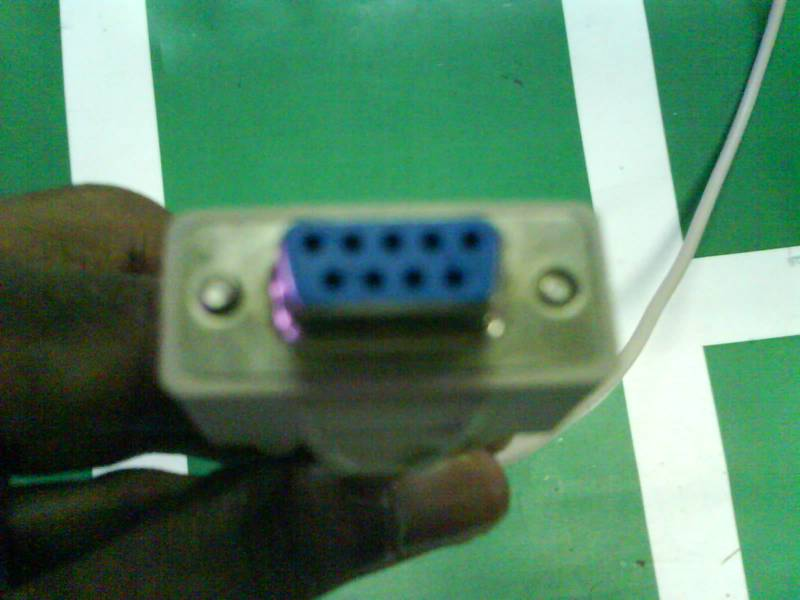
\includegraphics[width=0.5\linewidth]{RS232cable.jpg}
\caption{RS232 cable}
\end{figure}
\begin{figure}
\centering
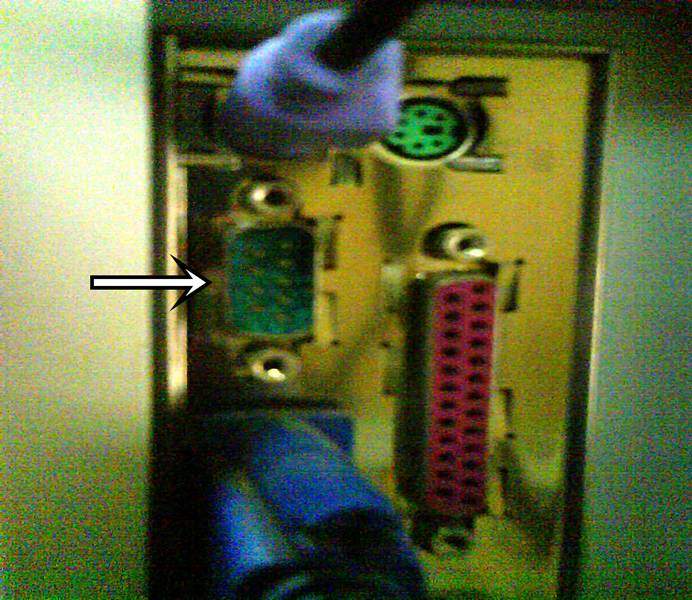
\includegraphics[width=0.5\linewidth]{Serialport.jpg}
\caption{Serial port}
\end{figure}
ATmega16 support a programmable Universal Synchronous and Asynchronous serial receiver and transmitter(USART) . Its baud rate is fixed at 9600 bps with character size set to 8 bits and parity bits disabled.
\subsection{Using USB for Communication}
After setting the jumper to USB mode connect the set up to the computer using a USB cable at appropriate ports as shown. To make the setup USB compatible USB to serial conversion is necessary. IC FT232R is used for this purpose.
\begin{figure}
\centering
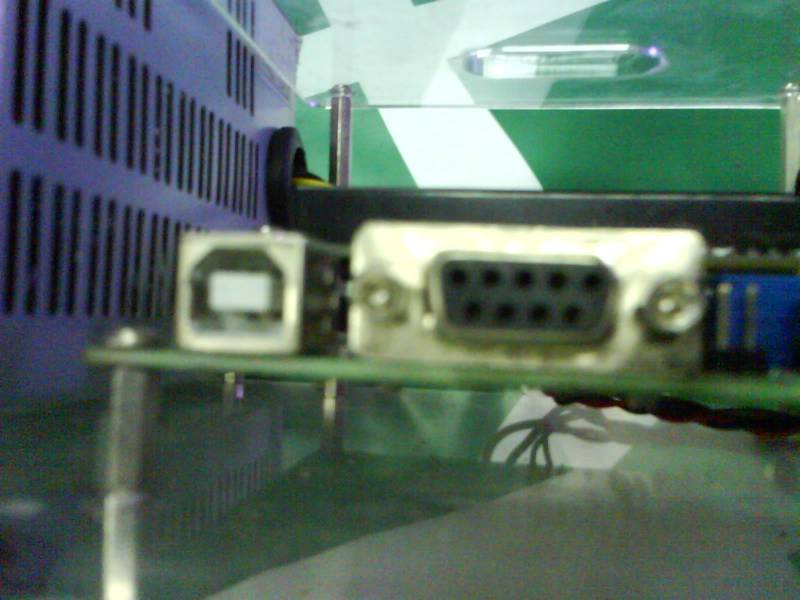
\includegraphics[width=0.5\linewidth]{usbc.jpg}
\caption{USB communication}
\end{figure}
\begin{figure}
\centering
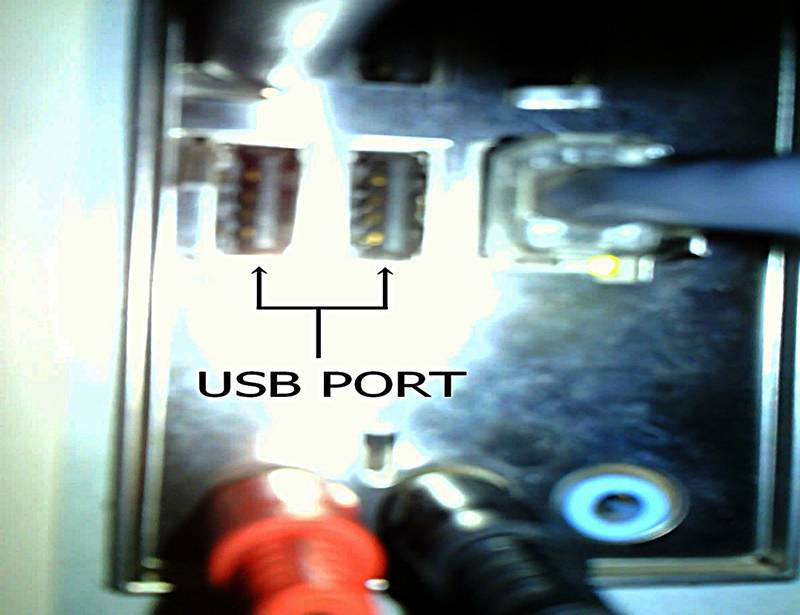
\includegraphics[width=0.5\linewidth]{usbp.jpg}
\caption{USB PORT}
\end{figure}
You need to have proper USB driver being installed on your computer.
\section{Display and Resetting the setup}
The temperature of the plate, percentage values of Heat and Fan and the machine identification number (MID) are displayed on LCD connected to the microcontroller.
As shown in figure, numerals below TEMP , indicate the actual temperature of the heater plate . Numeral below HEA and FAN indicate the respective percentage value at which heater and fan are being operated. Numerals below MID corresponds to the Device identification number.
\begin{figure}
\centering
\includegraphics[width=0.5\linewidth]{display.jpg}
\caption{Display}
\end{figure}

The set up could be reset at any time by pressing the reset button on it as shown in figure \ref{reset}. Reseting the setup takes it to the standby mode where the heater current is forced to be zero and fan speed to be the maximum value. Though these reset values are not displayed on the LCD display but they are loaded to the appropriate units. 
\begin{figure}
\centering
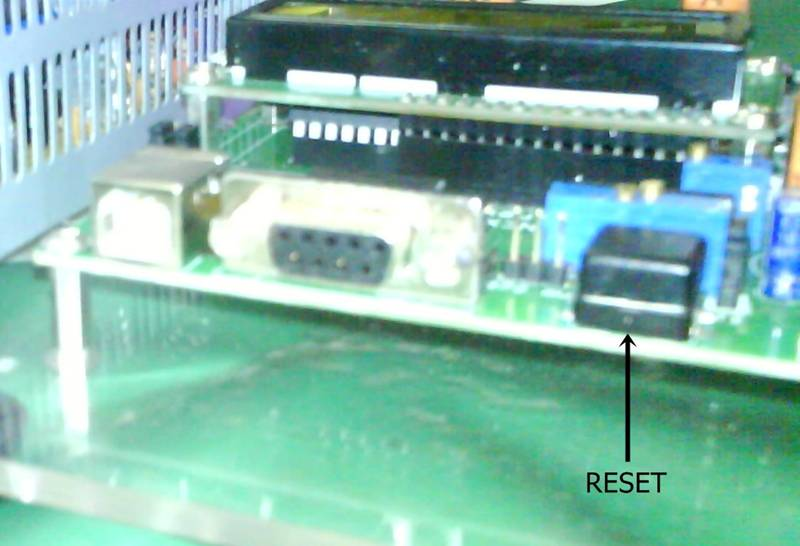
\includegraphics[width=0.5\linewidth]{r.jpg}
\caption{Reset}
\label{reset}
\end{figure}
\chapter{Using Scilab with Single Board Heater System}\label{sercomm}
This section explains the procedure to use Single Board Heater System with Scilab. An open loop experiment, step test is used for demonstrating this procedure. The process however remains the same for performing any other experiment explained in this document, unless specified. 
\section*{Hardware and Software Requirements}\label{umlauts}
For working with the Single Board Heater system, you would require the following:

\begin{enumerate}
\item SBHS with USB cable and power cable.
\item PC/Laptop with Scilab software installed (preferably the latest version). You may download it from:\\ {\tt http://www.scilab.org/products/scilab/download}
\item FTDI Virtual Com Port driver corresponding to the OS on your PC. (You may download it from: 
{\tt http://www.ftdichip.com/Drivers/VCP.htm})
\item Example StepTest provided along with this document.
\end{enumerate}
\section{Accessing Single Board Heater system on a Windows System}
\label{win_procedure}
This section deals with the procedure to use SBHS on a windows Operating System. The Operating System used for this document is Windows 7, 64-bit OS. In case if you are using some other Operating System or the steps explianed here are not sufficient to understand, you can refer to the official document available on  the main ftdi website. For doing so, go to www.ftdichip.com. On the left hand side panel, click on 'Drivers'. In the dropdown menu, choose 'VCP Drivers'. Then on the web page page, click on 'Installation Guides link'. Choose the required OS document. We would now begin with the procedure.
\subsection{Installing necessary driver and COM Port Settings}
After powering ON the SBHS and plugging in the USB cable to the PC (making sure you check the jumper settings on the board) for the very first time, the {\tt Welcome to Found New Hardware Wizard} dialog box pops up. You have to choose the option {\tt Install from a list or specific location}. Choose {\tt Search for best driver in these locations}. Check the button {\tt Include this location in the search}. Click on {\tt Browse}. Specify the path where you have copied the driver (item no.3) and install it by clicking {\tt Next}. Once the wizard has successfully installed the driver, your SBHS is ready for use. Please note that this procedure has to be repeated twice.

Now, we would check the communication port number assigned to the computer port to which you connect the Single Board Heater System, via an RS232 or USB cable.  For checking the port number, right click on My Computer and click on properties. Here, select the hardware tab and then click on Device Manager. You would see the list of hard ware devices. Look for Ports(COM \& LPT) option and open it. You would see the various communication port your computer is using. If you have connected RS232 cable, then look for Communications Port(COM1) else look for USB Serial Port. For RS232 connection, the port number mostly remains COM1. For USB connection it may change to some other number. Note the appropriate COM number. This process is illustrated in figure \ref{com_number}
\begin{figure}
\centering
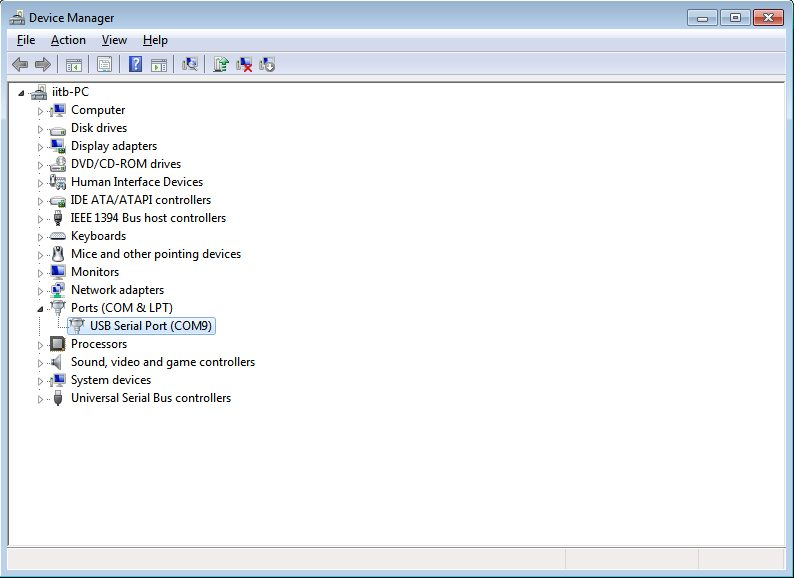
\includegraphics[width=0.7\linewidth]{COM.jpg}
\caption{Checking Communication Port number}
\label{com_number}
\end{figure}

Sometimes the COM port number you get after connecting a USB cable is more then single digit number 9. Since the serial tool box can handle only single digit port number, it is necessary to change your COM port number. Following is the procedure to do the same.
After following the procedure for knowing your com port number described above, double click that particular port. Click on Port Settings tab and then click on Advanced. In the COM port number dropdown menu, choose the port number to any other number less than 10. This procedure is illustrated in figure \ref{com_change}
\begin{figure}
\centering
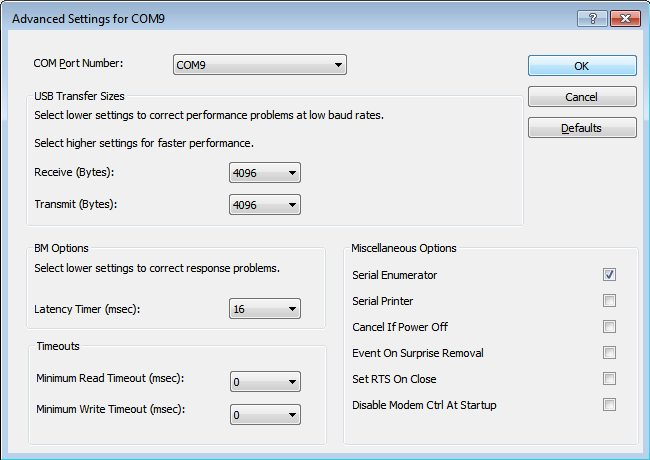
\includegraphics[width=0.7\linewidth]{port2.jpg}
\caption{Changing Com port number}
\label{com_change}
\end{figure}
\subsection{Configuring Scilab}
\label{scilab_sbhs}
Launch Scilab from start menu or double click the scilab icon on the desktop. Before executing any scripts which are dependent on other files or scripts, one has to change the working directory of scilab. Doing so will tell scilab from where it has to load the other necessary files. If you have other files saved to any other directory, you have to say {\ttfamily  getd<space>folder\_path} in the scilab console. Type {\ttfamily ls} to see the if the files are available. Here the directory is changed to the place where the relevent files for performiong step test resides. To change the directory, click on file menu and then choose "Change directory". You can also change the directory by typing {\tt cd<space>folder path}. Next, click on {\ttfamily editor} from the menu bar to open the scilab editor or simply type {\ttfamily editor} in the scilab console and open the file {\ttfamily ser\_init.sce}. Change the port number (the first argument of the {\tt openserial()} function) to the COM port number that you have noted down before. The second argument of the {\tt openserial()} function requires baud rate, parity, data bits and stop bits as a string.You should give it as {\tt "9600,n,8"}. Since stop bit is zero in our case, omit the parameter from the string to indicate it as zero. Execute this .sce file. You will get a message {\tt COM Port Opened}. If it complains, reconnecting the USB cable and/or restarting Scilab may help. Now execute the {\tt step\_test.sci} file.  The results are illustrated in figure \ref{loader}. 

\begin{figure}
\centering
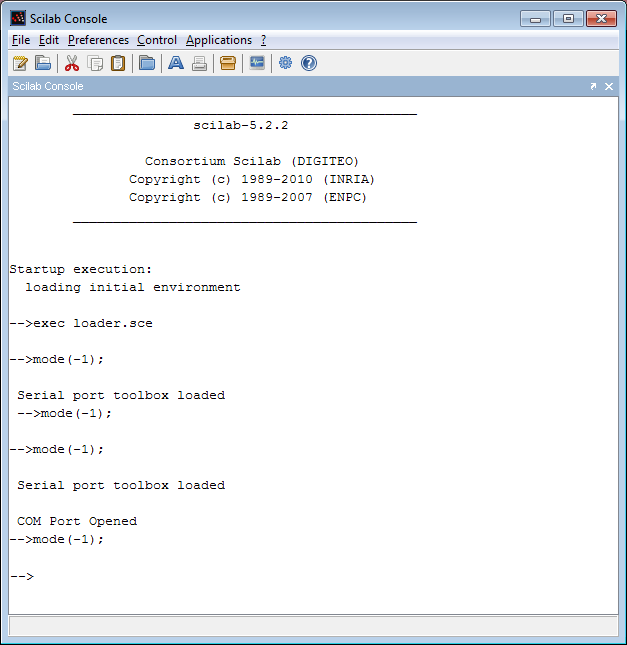
\includegraphics[width=0.7\linewidth]{console.png}
\caption{Expected responses seen on the console}
\label{loader}
\end{figure}


\begin{figure}
\centering
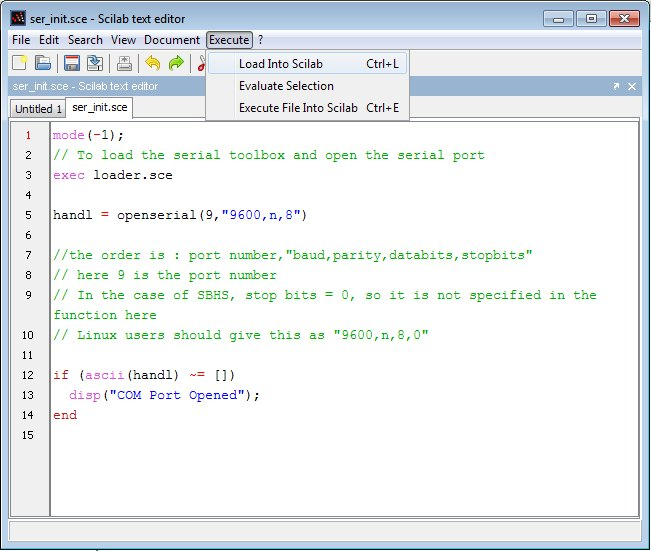
\includegraphics[width=0.7\linewidth]{scilab1.jpg}
\caption{Executing script files}
\label{exec}
\end{figure}


Type {\ttfamily Xcos} on the scilab console or click on Applications and choose {\ttfamily Xcos} to open Xcos environment. Load the {\ttfamily step\_test.xcos} file from the File menu. The Xcos interface that will open is as shown in figure \ref{Xcosintr}. You can set the block parameters by double clicking on the block as shown in figure \ref{blk_parameters}. To run the code click on Simulation menu and choose start. After running Xcos successfully you would see the plots as shown in figure \ref{plots}. See that the values of fan and heater you input to the xcos file is getting reflected on the board display. To stop the experiment click on the {\ttfamily stop} option on the menu bar of the Xcos environment.
\begin{figure}
\centering
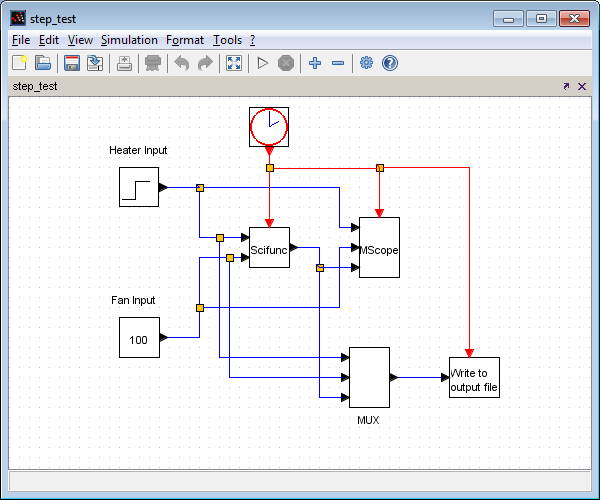
\includegraphics[width=0.7\linewidth]{xcos.png}
\caption{Xcos Interface}
\label{Xcosintr}
\end{figure}

\begin{figure}
\centering
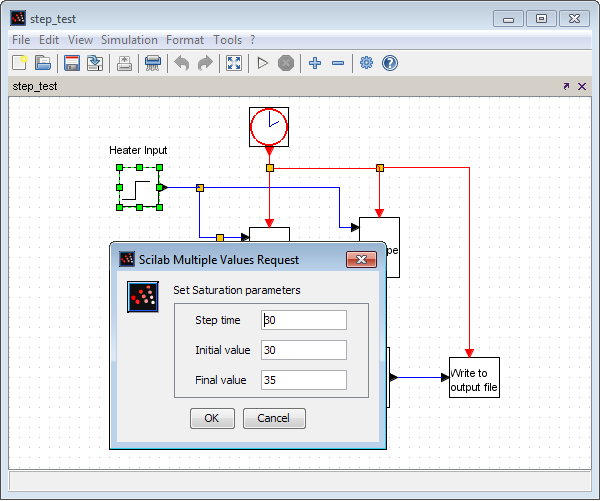
\includegraphics[width=0.7\linewidth]{xcos_block.png}
\caption{Setting Block Parameters}
\label{blk_parameters}
\end{figure}


\begin{figure}
\centering
\includegraphics[width=0.7\linewidth]{plot.png}
\caption{Plot obtained after executing step\_test.xcos}
\label{plots}
\end{figure}

\section{Accessing Single Board Heater system on a Linux System}
This section deals with the procedure to use SBHS on a Linux Operating System. The Operating System used for this document is Ubuntu 10.04.
For Linux users, the instructions given in section \ref{win_procedure} hold true with a few changes as below:

You do not require FTDI COM port drivers for connecting your SBHS to the PC. After plugging in the USB cable to your PC, check the serial port number by typing {\tt ls /dev/ttyUSB*} on the terminal, refer Fig.\ref{lstty}. Usually, the highest numbered one will be your device port number. eg:- {\tt /dev/ttyUSB0}. If you want to connect more than one USB device, then type {\tt tail -f /var/log/messages|grep ttyUSB} on the linux terminal just before plugging in the individual USB cable, refer Fig.\ref{tailusb}. The USB number will then be shown on the screen. Press {\tt Ctrl+ c} to abort the command. 
\begin{figure}
\centering
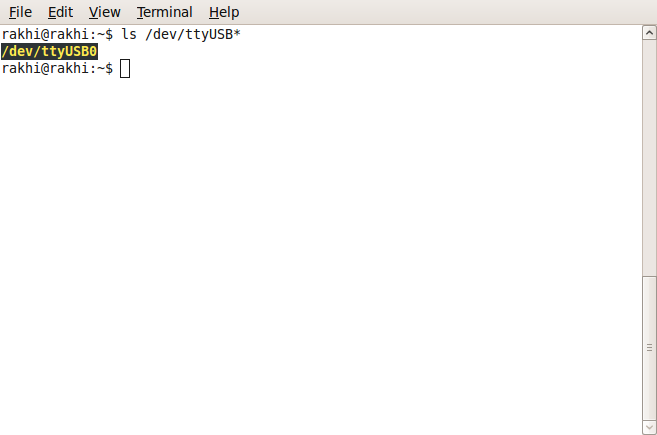
\includegraphics[width=0.7\linewidth]{lstty.png}
\caption{Checking the port number in linux (1)}
\label{lstty}
\end{figure}
\begin{figure}
\centering
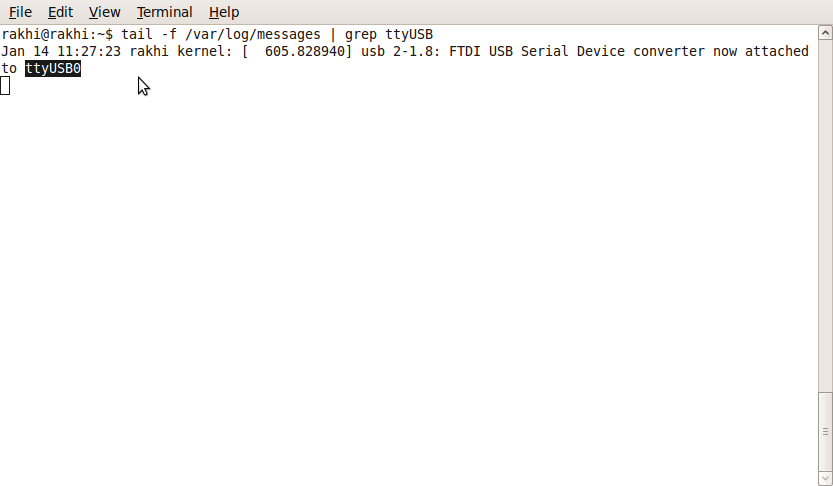
\includegraphics[width=0.7\linewidth]{tailusb.png}
\caption{Checking the port number in linux (2)}
\label{tailusb}
\end{figure}

Note this number and change the port number (the first argument of the \\ {\tt openserial()} function) in the {\tt ser\_init.sce} file with it. The second argument of the {\tt openserial()} function should be {\tt "9800,n,8,0"}, refer Fig.\ref{linuxserial}. This defines baud rate, parity, data bits and stop bits in that order. It has been found that if we omit the last parameter i.e., stop bits instead of specifying it as zero, scilab gives an error. Execute this file. Once the serial port initialisation is succesfully done, you get a message as shown in Fig.\ref{console_linux}. If it complains, reconnecting the USB cable and/or restarting Scilab may help.
\begin{figure}
\centering
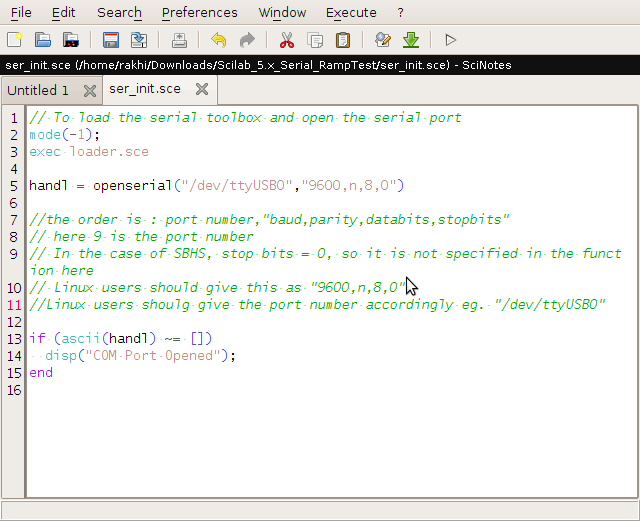
\includegraphics[width=\linewidth]{linuxserial.png}
\caption{Configuring port number and other parameters}
\label{linuxserial}
\end{figure}


\begin{figure}
\centering
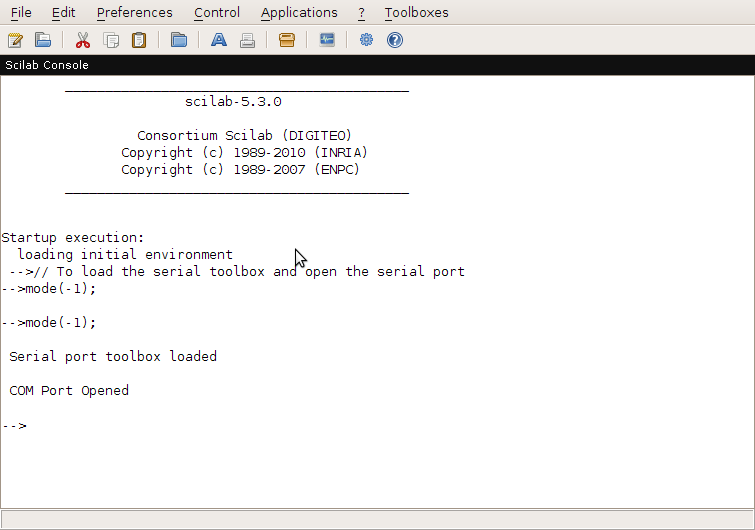
\includegraphics[width=0.7\linewidth]{SSscilab.png}
\caption{Scilab Console Message after Opening Serial Port}
\label{console_linux}
\end{figure}

Now execute the {\tt step\_test.sci} file.  The results are illustrated in figure \ref{loader}. Type {\ttfamily Xcos} on the scilab console or click on Applications and choose {\ttfamily Xcos} to open Xcos environment. Load the {\ttfamily step\_test.xcos} file from the File menu. The Xcos interface that will open is as shown in figure \ref{Xcosintr}. You can set the block parameters by double clicking on the block as shown in figure \ref{blk_parameters}. To run the code click on Simulation menu and choose start. After running Xcos successfully you would see the plots as shown in figure \ref{plots}. See that the values of fan and heater you input to the xcos file is getting reflected on the board display. To stop the experiment click on the {\ttfamily stop} option on the menu bar of the Xcos environment.
%Follow the instructions as given for Windows OS in section \ref{scilab_sbhs} for executing an example step test. This has been tested in Ubuntu Linux 10.04.


\chapter{Using Single Board Heater System, Virtually!}\label{virtual}
\section{Introduction to Virtual Labs at \\IIT Bombay}
The concept of virtual laboratory is a brilliant step towards strengthening the education system of an university/college, a metropolitan area or even an entire nation. The idea is to use the ICT i.e. Information and Communications Technology, mainly the Internet for imparting education or exchange of educational information. Virtual Laboratory mainly focuses on providing the laboratory facility, virtually. Various experimental set-ups are hooked up to the internet and made available to use for the external world. Hence, anybody can connect to that equipment over the internet and carry out various experiments pertaining to it. The beauty of this idea is that a college who cannot afford to have some experimental equipments can still provide laboratory support to their students through virtual lab, and all that will cost it is a fair Internet connection! Moreover, the laboratory work does not ends with the college hours, one can always use the virtual lab at any time and at any place assuming the availability of an internet connection. 

A virtual laboratory for SBHS is launched at IIT Bombay. Here is the url to access it: {\bf vlabs.iitb.ac.in/sbhs/}. A set of 36 SBHS are made available to use over the internet 24$\times$ 7. These individual kits are made available to the users on hourly basis. We have a slot booking mechanism to achieve this. Since there are 36 SBHS connected with an hours slot for 24 hrs a day, we have 864 one hour slots a day. This means that 864 individual users can access the SBHS in a day for an hour. This also means that up to 6048 users can use the SBHS for an hour in a week and 181440 in a month! A web page is hosted which is the first interface to the user. The user registers/logs in himself/herself here. The user is also supposed to book a slot for accessing the SBHS. A database server maintains a record of the data generated through the web interface. A python script is hosted on the server side and it helps in connecting the user with the corresponding SBHS placed remotely. A free and open source scientific computing Software, Scilab, is used by the user for implementing the experiment on SBHS, in terms of simple Scilab coding. 

\section{Evolution of SBHS virtual labs}
In \cite{vlabs-kmm}, 
the control algorithm is implemented at the server end and the remote
student just keys in the parameters, as shown in Figure
\ref{fig:initial}. 
\begin{figure}
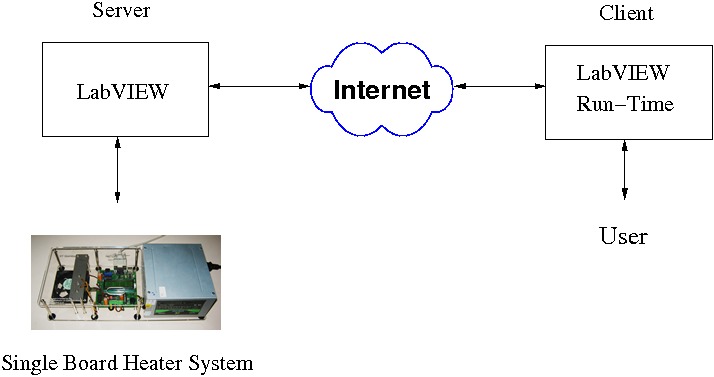
\includegraphics[width=\linewidth]{vlabs/vlab-1.png}
\caption{SBHS virtual laboratory with remote access using LabVIEW}
\label{fig:initial}
\end{figure}
LabVIEW was used for the implementation of the same. The
server end consisted of a computer connected with an SBHS with a full
blown copy of LabVIEW installed on it. The client has a LabVIEW run
time engine available for free download from the National Instruments
website.  A few
LabVIEW algorithms/experiments were hosted on the server. The client
accesses these algorithm/experiment over the Internet using a web
browser by entering appropriate parameters.

It was realized that the learning experience is not complete for this
structure. This is because the server hosts some pre-built LabVIEW
algorithms and a user can only access these few algorithms. The user
can in no way change the program and can only input experimental
parameters. 
Hence, we came up with a new architecture
as shown in the Figure \ref{fig:second} that used full blown copies of
LabVIEW at both server and client ends.  
\begin{figure}
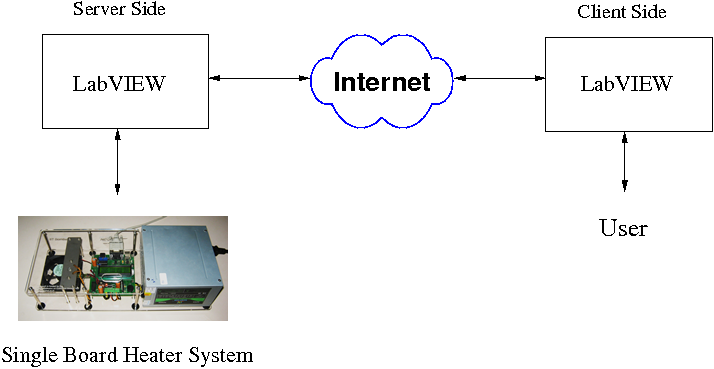
\includegraphics[width=\linewidth]{IEEE-Chile/figures/vlab-2.png}
\caption{SBHS virtual laboratory with remote access and live data sharing using LabVIEW}
\label{fig:second}
\end{figure}
 
 This idea uses the DataSocket technology of LabVIEW. Since now the
 client is having a complete LabVIEW installation on his/her computer
 she can now implement her own algorithms.  Thus this architecture did
 provide a complete learning experience to the students.  There are
 some shortcomings as well:

\begin{itemize}
\item LabVIEW is expensive and students may not be able to afford to
  buy it.  It is also prohibitively expensive for the Government to
  distribute it.

\item We used the LabVIEW version 8.04, which had restricted scripting
  language.  It was tedious to create new control algorithms in it.
\end{itemize}
\begin{figure}
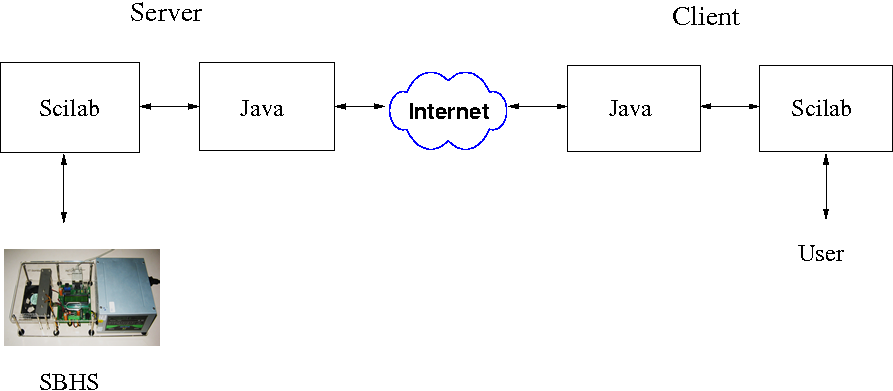
\includegraphics[width=\linewidth]{vlabs/vlab-3.png}
\caption{SBHS virtual laboratory using open source software}
\label{fig:third}
\end{figure}
This made us shift to free and open source (FOSS) software. We
replaced LabVIEW with Java and Scilab as shown in Figure
\ref{fig:third}. Scilab at the server end is used for communicating
with SBHS. Scilab at the client end is used for implementing the
algorithms. Java is used at both the server as well as client end for
communication over the Internet thereby connecting the client with the
server. 

For the above solution, we need a dedicated copy of scilab running at
the server end for every SBHS. One way to do this is to host it on
multiple computers with unique IPs. Hence the number of SBHS we want
to host requires as many computer's and public IPs thereby making
it expensive. Moreover, it also limits its scalability. The other way
to do this is to host multiple java and scilab servers on the same
computer.  Hosting many copies of Scilab simultaneously requires a
powerful computer for the server.

For these reasons  we decided to take scilab off the server computer
and to use java alone to communicate with the SBHS directly.  Java
also 
communicates with the client computer.  We connected seven SBHS
systems to a USB port through a serial port hub.  This architecture
was 
implemented on a Windows Operating System.  We faced the following
difficulties in this solution.
\begin{itemize}
\item When we connected more than one serial hub to a PC, the port ID
  could not be retrieved correctly.  Port ID information is required
  if we want a student to use the same SBHS for all their experiments
  during different sessions.
\item The experiments required time stamping of the data communicated
  to and from the server. But this time stamping was not linear and
  suffered instability.  
\end{itemize}
This made us to completely switch to FOSS with Ubuntu Linux as the OS
and is the current structure of the Virtual lab as shown in Figure
\ref{fig:detail-arch} 

\begin{figure}
\centering
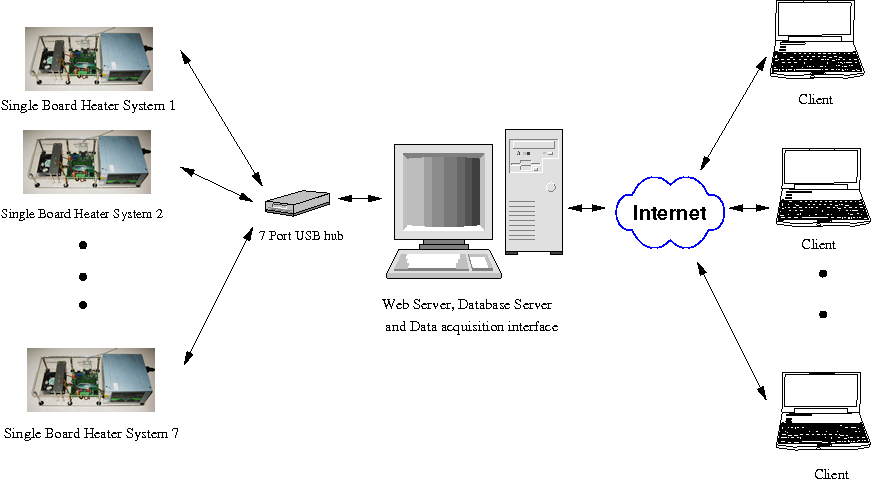
\includegraphics[width=\linewidth]{vlabs/vlab-arch}
\caption{Virtual control lab hardware architecture}
\label{fig:hw-arch}
\end{figure}

\section{Current Hardware Architecture}
The current hardware architecture of the virtual single-board heater system lab involves 36 single-board heater systems connected to the server via multiple 7 and 10-port USB hubs. The server computer is connected to a high speed internetwork and has enough processing capability to host data acquisition, database, and web servers. 
It has been successfully tested for the undergraduate Process Control course and the graduate Digital Control and Embedded systems courses conducted at IIT Bombay as well as few workshops over the internet. Currently, this architecture is integrated with a cameras on each SBHS to facilitate live video streaming. This gives the user a feel of remote hands-on. 

\section{Current Software Architecture} \label{sec:vlabarchi}
The current software architecture of this virtual SBHS control lab is shown in Figure \ref{fig:detail-arch}. The server computer runs Ubuntu Linux 12.04.2 OS. It hosts a Apache-MySQL server. The SBHS server is based on Python-Django framework and is linked to Apache server using Apache's WSGI module. The MySQL database server has the details of all the registered users, their slot details, authentication keys to allow remote access, etc. As shown in Figure \ref{fig:sbhs-website}, the Python-Django server has pages for registration, login, slot booking etc. \cite{vl010}.  On the client end, control algorithms are running in Scilab and a python based client application communicates with virtual labs server over the Internet.



\begin{figure}
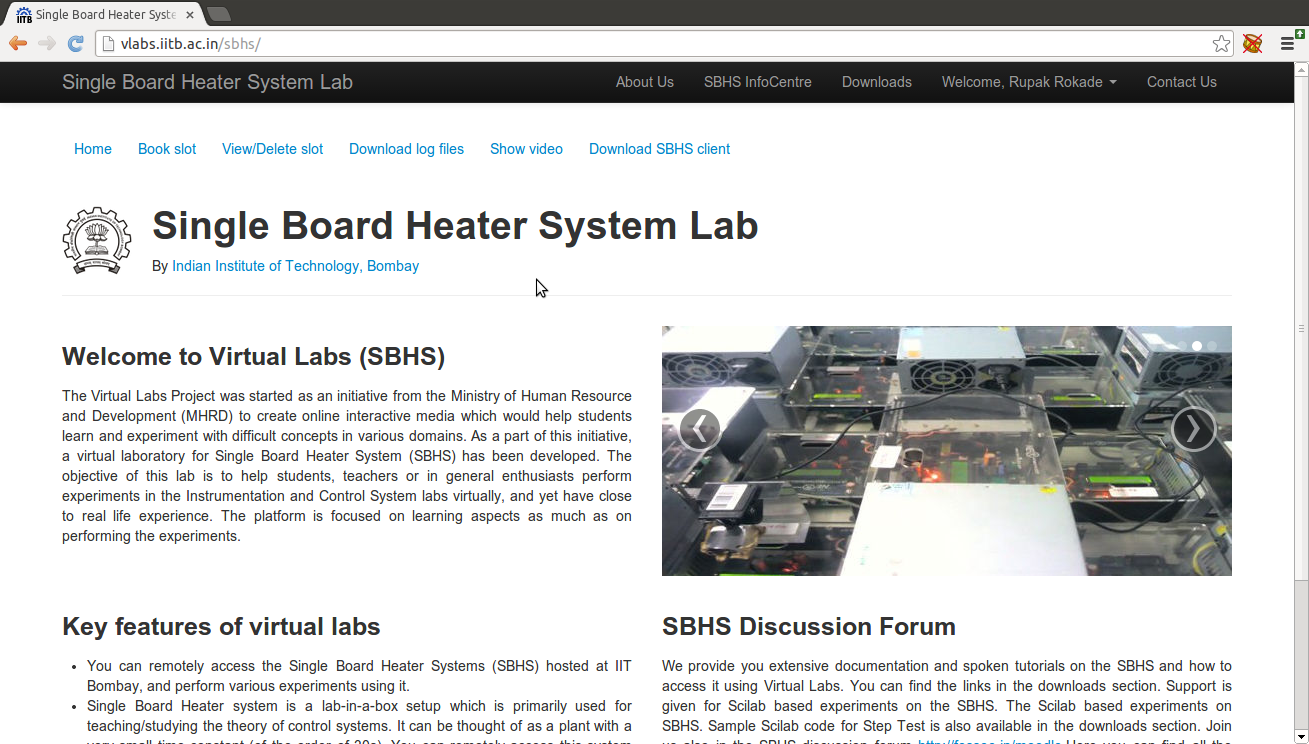
\includegraphics[width=\linewidth]{vlabs/webpage}
\caption{Home page of SBHS V Labs}
\label{vlabs-home}
\end{figure}
The steps to be performed before and during each experiment are explained next.

\begin{figure}
\centering
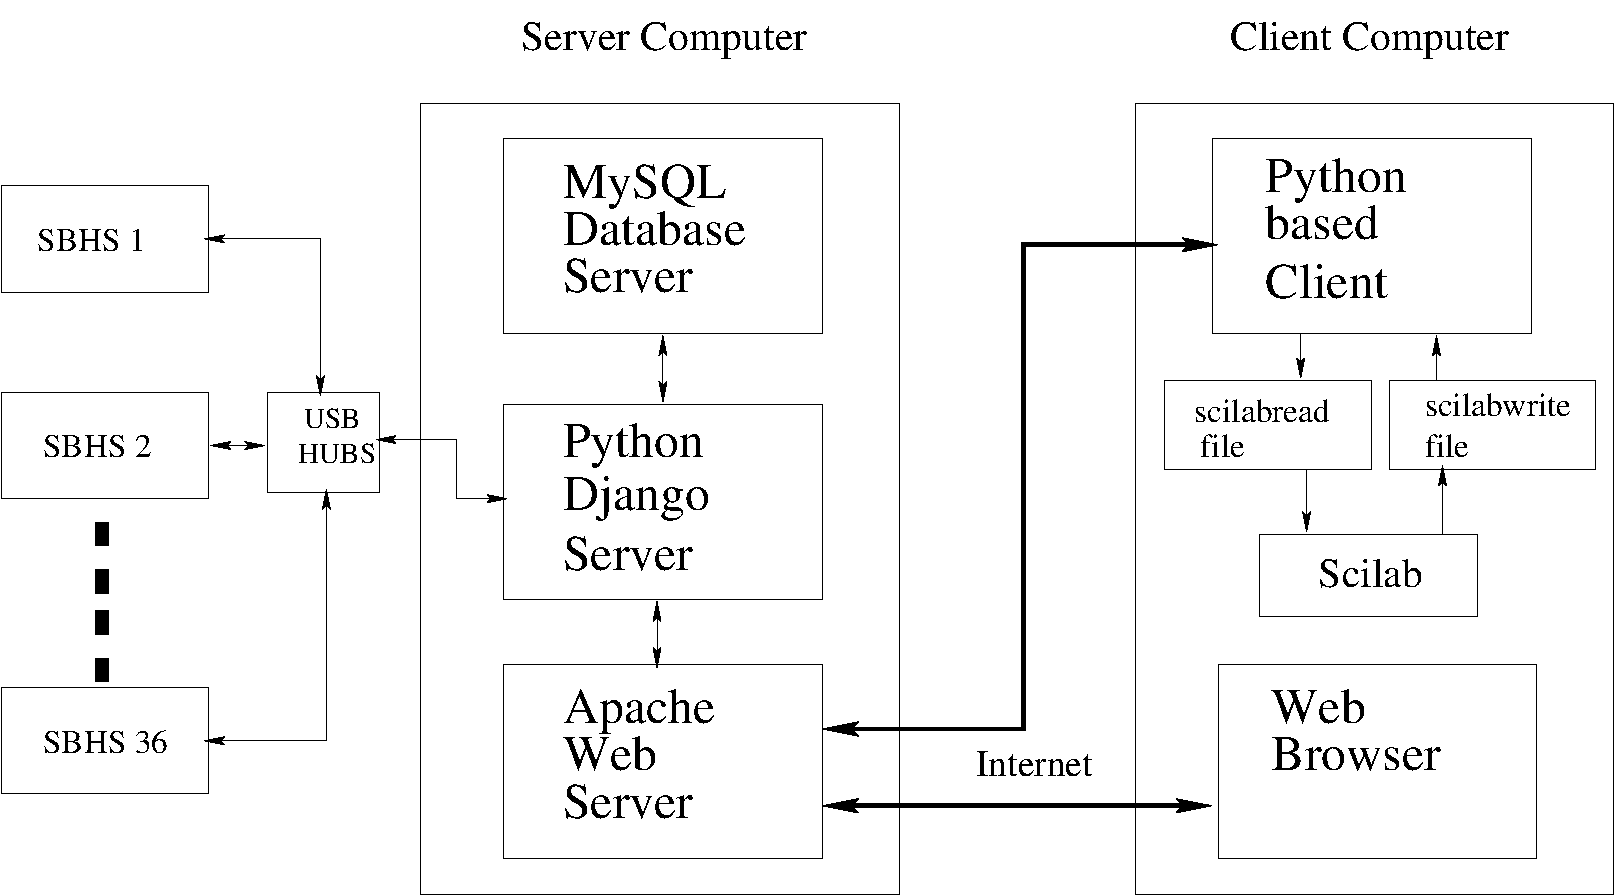
\includegraphics[width=\linewidth]{vlabs/new-server-arch.pdf}
\caption{Current Architecture of SBHS Virtual Labs}
\label{fig:detail-arch}
\end{figure}

\section{Conducting experiments using the Virtual lab}\label{vlabsexpt}

This section explains the procedure to use Single Board Heater System remotely using Scilab i.e. when you are accessing SBHS remotly using your computer over the virtual labs platform. An open loop experiment, step test is used for demonstrating this procedure. The process however remains the same for performing any other experiment explained in this section, unless specified otherwise. Let us first see the required files to be downloaded and installations to be done. Scilab is required to be installed on your computer. Please refer to Section \ref{driver} and Section \ref{linux-sbhs} for the procedure to install scilab on Windows and Linux system, respectively.

SBHS scilab code for your OS,  under the section {\tt SBHS Virtual Code}, must be downloaded from {\tt http://sbhs.os-hardware.in/downloads}. For example, if you are using a 32-bit linux operating system then you should download the file {\tt SBHS Scilab codes for Linux - (32 bit)}. The code downloaded will be in zip format. After the zip is unpacked, you will see scilab experiment folders such as {\tt Step\_test}, {\tt Ramp\_Test}, {\tt pid\_controller} etc. We will be using the {Step\_test} folder. Do not alter the directory structure. If you want to copy or move an experiment outside the directory then make sure you also copy the {\tt common\_files} folder. The {\tt common\_files} folder must always be one directory outside the experiment folder. Now given that you have scilab installed and working and the required scilab code downloaded, let us see the step-by-step procedure to do a remote experiment.

\subsection{Registration, Login and Slot Booking}\label{regAndslot}
 Go to the website {\tt sbhs.os-hardware.in} and click on the {\tt Virtual labs} link available on the left hand side. The home page of Virtual labs is illustrated in Fig \ref{vlabs-home}. If you are a first time user, click on the link {\tt Login/Register}. Fill out the registration form and submit it. If the registration form is submitted successfully, you will receive an activation link on your registered Email id. Use this link to complete the registration process. If you skip this step you will not be able to login. Registration is a one time process and need not be repeated more than once. After completing registration login with your username and password. You should now get the options to Book Slot, Delete Slot etc. 

View/Delete slot option allows you to delete your booked slots. This option however will work only for slots booked for the future. You cannot delete a past or the current slot. Download log files option gives you the facility to download your experiment log files. Clicking on it will give you a list of all of the experiments you had performed. Show video option can be used to see the live video feed of your SBHS. Web cameras are mounted on every SBHS. You can see the display of your SBHS as shown in Fig. \ref{web-cam}.

\begin{figure}
\centering
\includegraphics[width=0.5\linewidth]{vlabs/display.jpg}
\caption{Show Video}
\label{web-cam}
\end{figure}

Clicking on the Book slot option will allow you to book an experiment time slot. Slots are of 55 minutes duration. Click on the Book slot option. If the current slot is free, Book now option will appear. Click on it. Else you have to book an advance slot for the next hour or any other future time using the calender that appears on this page. There is a limit to how many slots one can book in a day. We are allowing only two non-consecutive slots, per user, to be booked in a day. However, there is no limit to how many current slots you book and use. Book an experiment slot. Once you successfully book a slot a {\bf Slot booked successfully} message highlighted in green color will appear on the top side. This is shown in Fig. \ref{book-slot}. It will automatically take you to the View/Delete slot page.

\begin{figure}
\centering
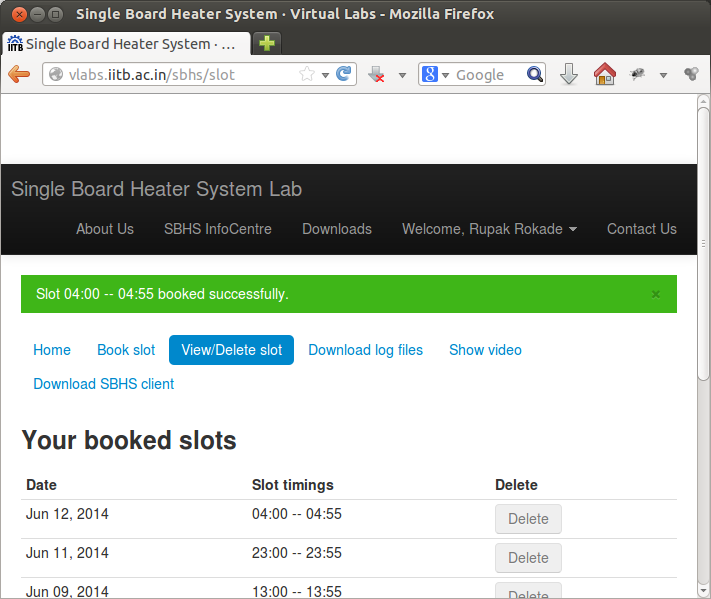
\includegraphics[width=0.7\linewidth]{vlabs/book-slot.png}
\caption{Slot booking}
\label{book-slot}
\end{figure}

\subsection{Configuring proxy settings and executing python based client}\label{proxy}
After booking a slot, the web activity is over. You may close the web browser unless you need it open to see live video feed of your SBHS. The next step is to establish the communication link between the server and your computer. A python based application is created which handles the network communication. 

Let us first see how to do the proxy  settings if you are behind a proxy network. Open the folder {\tt common\_files}. Open the file {\tt config}. This files contains various arguments whose values must be eneterd to configure proxy. 

{\bf Do not change the contents of {\tt config} file if}
\begin{itemize}
\item You are accessing from inside IIT Bombay OR
\item You are accessing from outside IIT Bombay and using an open network such as at home OR using a mobile internet
\end{itemize}

{\bf Change the contents of {\tt config}  file if}
\begin{itemize}
\item You are outside IIT Bombay and using a proxy network such as at an institute, office etc.
\end{itemize}

If you have to put the proxy details, first change the argument {\tt use\_proxy} = Yes (Y should be capital in Yes and N should be capital in No). Fill in the other details as per your proxy network. If your proxy network allows un-authenticated login then make the argument {\tt proxy\_username} and {\tt proxy\_password}  blank. This proxy setting has to done only once.

Open the {\tt Step\_test} folder. Double click on the file {\tt run}. This will open the client application as shown in Fig. \ref{python-client}. Note that for first time execution, it will take a minute to open the client application. It will show various parameters related to the experiment such as SBHS connection, Client version, User login and Experiment status. The green indicators show that the corresponding activity is correct or functional. Here it says that the Client application is been able to connect to the server and the client version being used is the latest. The User login and Experiment status is showing red and will turn green after a registered username and password is entered. If the SBHS is offline or there are some other issues, the corresponding error will be displayed and the respective indicator will turn red. Enter your registered username and password and press login. You should get the message {\tt Ready to execute scilab code}. The application also shows the value of iteration, heat, fan, temperature and time remaining for experimentation. It also shows the name of log file created for the experiment.

\begin{figure}
\centering
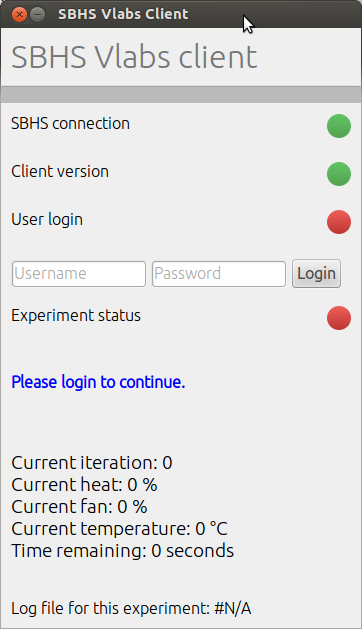
\includegraphics[width=0.5\linewidth]{vlabs/python-client.png}
\caption{Python Client}
\label{python-client}
\end{figure}


\subsection{Executing scilab code}
Inside the {\tt StepTest} folder, if on a windows system, double click on the  file {\tt stepc.sce}. This should automatically launch scilab and also open the {\tt stepc.sce} in the scilab editor. It will also automatically change the scilabs working directory. On a linux system, launch scilab manually. Then change the scilab working directory to the folder {\tt StepTest}. This can be done by clicking on {\tt File} menu and then selecting {\tt change current directory}. Next, execute the command {\tt getd ..\slash common\_files}. Scilab command {\tt getd} is used to load all functions defined in all .sci files inside a specified folder. Here we have some important function files inside the {\tt ..\slash common\_files} directory. Executing this command will load all of the functions that the experiment needs. Open the file {\tt stepc.sce} using the {\tt Open} option inside {\tt File} menu. The file is shown in Fig. \ref{stepc}

\begin{figure}
\centering
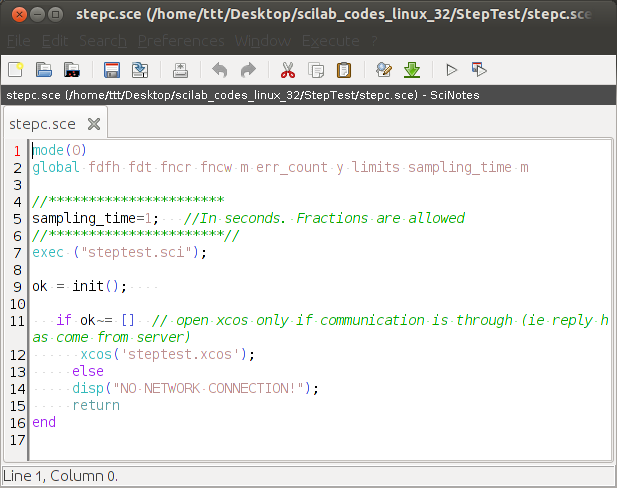
\includegraphics[width=0.7\linewidth]{vlabs/stepc.png}
\caption{stepc.sce file}
\label{stepc}
\end{figure}

The experiment sampling time can be set inside the  {\tt stepc.sce} file. You may want to change it to a higher value if your network is slow. The default value of 1 second works fine in most cases. On the menu bar, click on {\tt Execute} option and choose option {\tt file with echo}. This will execute  the scilab code. If the network is working fine, an xcos diagram will open automatically. If it doesnt open then see the scilab console for error messages. If you get a {\tt No network connection} error message then try executing the scilab code again. The xcos diagram is for the step test experiment as shown in Fig. \ref{step-xcos}. You can set the value of the heat and fan. Keep the default values. On the menu bar of the xcos window, click on {\tt start} button. This will execute the xcos diagram. If there is no error, you will get a graphic window with three plots. It will show the value of Heat in \% Fan in \% and ..temperature in degree celcius as shown in Fig. \ref{step-plot}. After sufficient time of experimentation click on the stop button to stop the experiment. Go to the {\tt StepTest} folder. Here you will find a {\tt logs} folder. This folder will have another folder named after your username. It will have the log file for your experiment. Read the log file name as\\ YearMonthDate\_hours\_minutes\_seconds.txt. This log file contains all the values of heat fan and temperature. It can be used for further analysis.

\begin{figure}
\centering
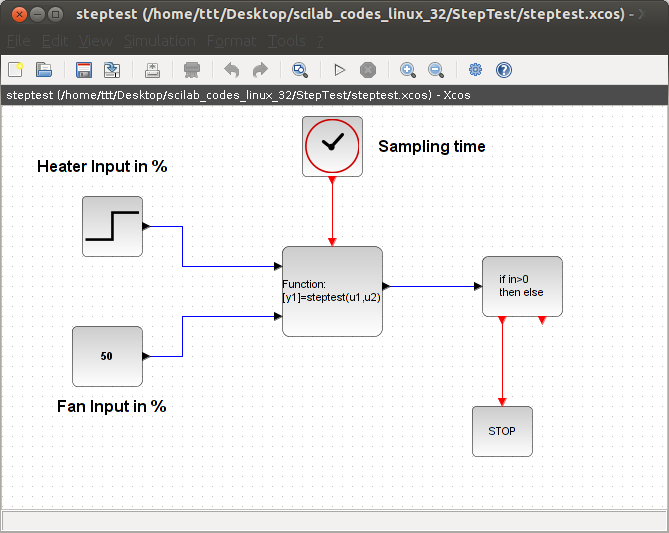
\includegraphics[width=0.7\linewidth]{vlabs/step-xcos.png}
\caption{Xcos for step test}
\label{step-xcos}
\end{figure}

\begin{figure}
\centering
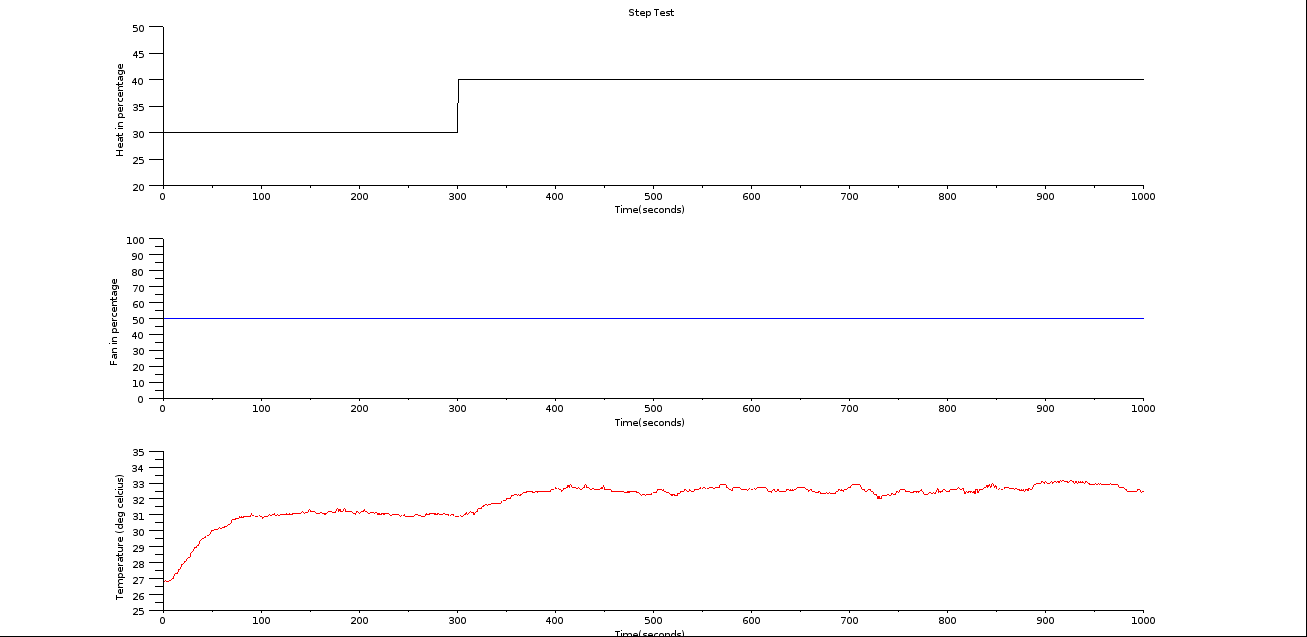
\includegraphics[width=0.7\linewidth]{vlabs/step-test-output.png}
\caption{Output of Step Test}
\label{step-plot}
\end{figure}

\section{Summary}\label{virtual-summary}

This section summarizes the process to perform an experiment on SBHS using virtual lab interface. This section assumes that the user has already created an account and booked a slot as explained in section \ref{regAndslot}. It also assumes that the proxy settings are already done as explained in section \ref{proxy}. The user should follow these steps within the booked slot time.
\begin{itemize}
\item Step1: Open the StepTest experiment directory
\item Step2: Double-click on the file {\tt run}. Expect the SBHS cient application to open.
\item Step3: Enter the username and password inside the SBHS cient application and press {\tt login} button. Expect the message {\tt Ready to execute scilab code}
\item Step4: Switch to the StepTest experiment directory and double-click on the file {\tt stepc.sce}. This will launch scilab and also open the file {\tt stepc.sce} in the scilab editor. Linux users will have to launch scilab manually. They also have to change the working directory to StepTest and then open the {\tt stepc.sce} file in the scilab editor.
\item Step5 Switch to the scilab console and execute the command {\tt getd ..\slash common\_files}
\item Step6: Execute the file {\tt stepc.sce}. Expect the step test xcos diagram to open automatically. If this doesnt happen, check the scilab console for error message.
\item Step7: Execute the step test xcos daiagram. You may change the input parameters, if required, before executing. Expect a plot window to open automatically showing three graphs.
\item Step8: Stop the Xcos simulation after the experiment is completed properly. 

\end{itemize}
\chapter{Identification of Transfer Function of a Single Board Heater System through Step Response Experiment}\label{chap1}
The aim of this experiment is to perform step test on a Single Board Heater System and to identify system transfer 
function using step response data. The target group is anyone who has basic knowledge of control engineering.

\begin{figure}
\centering
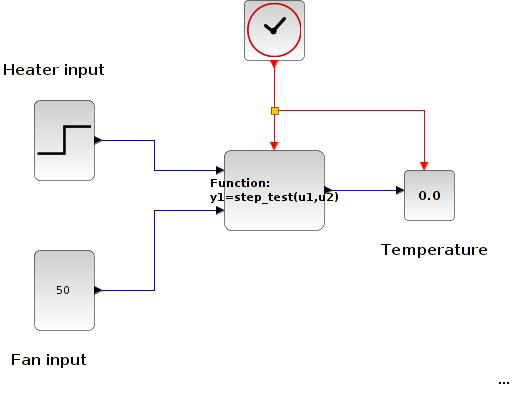
\includegraphics[width=\linewidth]{Step-test_manual/step_xcos.jpg}
\caption{Xcos for this experiment}
\label{xcos_st}
\end{figure}

\begin{figure}
\centering
\includegraphics[width=\linewidth]{Step-test_manual/plot}
\caption{Graph shows heater current, fan speed and output temperature}
\label{fig:scope_st}
\end{figure}

We have used Scilab and Xcos as an interface for sending and receiving data. 
Xcos diagram is shown in figure \ref{xcos_st}. Heater current and fan speed are the two inputs for this system. 
They are given in percentage of maximum. These inputs can be varied by setting the properties of the input block's properties 
in Xcos. The plots of their amplitude versus number of collected samples are also available on the scope windows. 
The output temperature profile, as read by the sensor, is also plotted. The data acquired in the process is stored on the 
local drive and is available to the user for further calculations.

\section{Procedure to perform Step Test}
The procedure to perform a step test is explained in section \ref{scilab_sbhs}.\\ In the 
{\tt step\_test.xcos} file, open the heater block's parameters to apply a step change of 
say 5 percent to the heater at operating point of 30 percent of heater after 200 seconds. The block 
parameters of the step input block will have {\tt Step time = 200}, {\tt Initial value = 30} and {\tt Final value = 35}. 
Keep the fan input constant at 50 percent. Start the experiment and let it continue until you see the temperature 
reach the steady state. 

\begin{table}
\begin{verbatim}
 0.100E+00  0.300E+02  0.50E+03  0.195E+02
 0.200E+00  0.300E+02  0.50E+03  0.195E+02
.
.
 0.700E+03  0.350E+02  0.50E+03  0.318E+02
 0.800E+03  0.350E+02  0.50E+03  0.318E+02
\end{verbatim}
\caption{Step data obtained after performing the Step Test}
\label{stepdata}
\end{table}

The step test data file is saved in {\tt Step\_test} folder. The name of the file will be the date and time at which the 
experiment was conducted. Referring to the data file thus obtained as shown in table \ref{stepdata}, the first column in this 
table denotes samples. The second column in this table denotes heater in percentage. It starts at 30 and increases with a step size 
of 5 units. The third column denotes the fan in percentage. It has been held constant at 50 percent. The fourth column refers to the 
value of temperature.


\section{Determination of First Order Transfer Function}
Identification of the transfer function of a system is important as it helps us to 
represent the physical system mathematically. Once the transfer function is obtained, one can acquire 
the response of the system for various inputs without actually applying them to the system.

Consider the standard first order transfer function given below
\begin{align}
G(s) &= \frac{ C(s)}{ R(s)}\label{1}\\
G(s)&=\frac 1{\tau s+1}\label{std_fo}                           
\intertext{Rewriting the equation, we get}
C(s)  &= \frac {R(s)}{\tau s + 1}\label{rw_std_fo}
\intertext{A step is given as input to the first order system. The Laplace 
transform of a step function is$ \frac {1}{s}$. Hence, substituting $ R(s) = \frac {1}{s}$ in equation \ref{rw_std_fo}, 
we obtain}
C(s) & = \frac 1{\tau s + 1}\frac 1{s}\label{sub_rs}\\
\intertext{Solving $C(s)$ using partial fraction expansion, we get}
C(s) &= \frac1{s} - \frac {1}{s + \frac1 \tau}\label{pf}
\intertext{Taking the Inverse Laplace transform of equation \ref{pf}, we get}
c(t)&= 1 - e^{\frac {-t}\tau }\label{lti} 
\end{align}
From the above equation it is clear that for t=0, the value of c(t) is zero. For t= $\infty$, c(t) 
approaches unity. Also, as the value of \textquoteleft t \textquoteright  becomes equal to $\tau$, 
the value of c(t) becomes 0.632. $\tau$ is called the time constant and represents the speed of 
response of the system. But it should be noted that, smaller the time constant- faster the system response.
By getting the value of $\tau$, one can identify the transfer function of the system. 

Consider the system to be first order. We try to fit a first order transfer function of the form
\begin{align}       
G(s) &= \frac K{\tau s + 1}\label{7}
\intertext{to the Single Board Heater System. Because the transfer function approach uses deviation 
variables, $ G(s)$ denotes the Laplace transform of the gain of the system between the change in heater 
current and the change in the system temperature. Let the change in the heater current be denoted by $\Delta u$.  
We denote both the time domain and the Laplace transform variable by the same lower case variable. Let the change 
in temperature be denoted by $y$. Let the current change by a step of size $u$. Then, we obtain the following 
relation between the current and the temperature.} 
y(s) &= G(s)u(s)\\ 
y(s)&= \frac K{\tau s + 1}{\frac  {\Delta u}{{s}}}
\intertext {Note that $\Delta$ u is the height of the step and hence is a constant. On inversion, we obtain}
y(s)&= K[1 - e^{\frac{-t}\tau}]\Delta u
\end{align}
\subsection{Procedure}
\begin{enumerate}
 \item Copy the step test data file to the folder {\tt Kp-tau-order1}.
 \item Change the Scilab working directory to {\tt Kp-tau-order1} folder under {\tt Step\_Analysis} folder.
 \item Open the file {\ttfamily firstorder.sce} and place the name of the data file 
with extention in the filename field. 
\item Save and run this code and obtain the plot as shown in figure \ref{firstorder_output}. 
\end{enumerate}
This code uses the routines {\ttfamily label.sci} and {\ttfamily costf\_1.sci}

\begin{figure} 
\centering
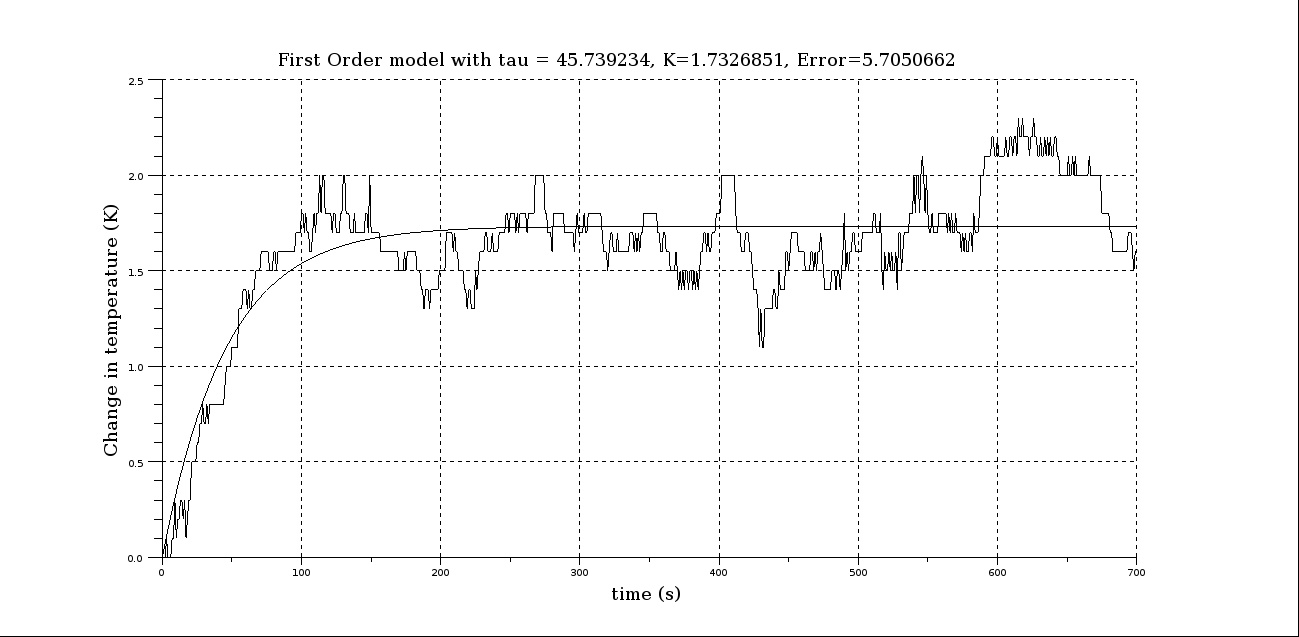
\includegraphics[width=\linewidth]{Step-test_manual/step_first_order.jpg}
\caption{Output of the Scilab code \ttfamily firstorder.sce}
\label{firstorder_output}
\end{figure} \label{firstorderplot}

\begin{align}
\intertext{The plot thus obtained is reasonably good. See the Scilab plot to get the values of $\tau$ and $K$. 
The figure \ref{firstorder_output} shows a screen shot of the same. We obtain $\tau$ = 45.739234, K = 1.7326851. The transfer function 
obtained here is at the operating point of 30 percentage of heat. If the experiment is repeated at a different operating point, 
the transfer function obtained will be different. The gain will correspondingly be more at a higher operating point. 
This means that the plant is faster at higher temperature. Thus the transfer function of the plant varies with the operating 
point. Let the transfer function we obtain in this experiment be denoted as $G_s$. We obtain}
G_s(s) =  \frac{1.7326851}{45.739234s+1} \label{12}
\end{align}
% \begin{figure}
% \centering
% 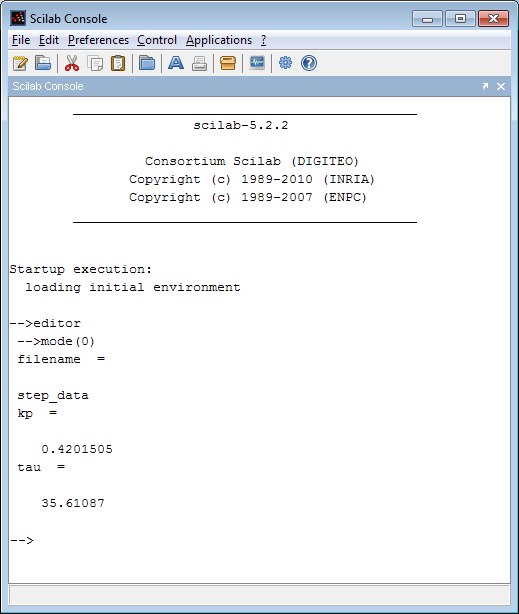
\includegraphics[width=\linewidth]{Step-test_manual/forder_console.png}
% \caption{The value of time constant and gain as shown on the console by \ttfamily firstorder.sce}
% \label{console}
% \end{figure}


\section{Determination of Second Order Transfer Function}
In this section, we explore the efficacy of a second order model of the form
\begin{align}
G(s) & = \frac K{(\tau_1s+1)(\tau_2s+1)} \label{eq:step-1100} 
\intertext{The response of the system to a step input of height $\Delta u$ is given by}
y(s) & = \frac K{(\tau_1s+1)(\tau_2s+1)} \frac{\Delta u}s 
\label{eq:step-1200} 
\end{align}

Splitting into partial fraction expansion, we obtain
\begin{align*}
y(s) & = \frac K{\tau_1\tau_2} \frac 1
{\left(s+\dfrac 1{\tau_1}\right)\left(s+\dfrac 1{\tau_2}\right)} =
\frac A s + \frac B{s+\dfrac 1{\tau_1}} + \frac C{s+\dfrac 1{\tau_2}}
\intertext{Through Heaviside expansion method, we determine the coefficients:}
A & = K \\
B & = -\frac{K\tau_1}{\tau_1-\tau_2} \\
C & = \frac{K\tau_2}{\tau_1-\tau_2}
\end{align*}

On substitution and inversion, we obtain
\begin{align}
y(t) & = K\left[ 1 - \frac 1{\tau_1-\tau_2}
\left( \tau_1 e^{-t/\tau_1} - \tau_2 e^{-t/\tau_2} \right)
\right] \label{eq:step-1300}
\end{align}

We have to determine three parameters $K$, $\tau_1$ and $\tau_2$
through optimization. Once again, we follow a procedure identical to the first order model.  
The only difference is that we now have to determine three parameters. Scilab code \\{\tt secondorder.sce} calculates
the gain and two time constants. 
\subsection {Procedure}
\begin{enumerate}
 \item Change the Scilab working diectory to the folder {\tt Kp-tau-order2}.
 \item Copy the step test data file to this folder. 
 \item Run the code {\tt secondorder.sce} with the appropriate data file name. 
\end{enumerate}
The plot shown in figure \ref{sorder} is obtained.  It corresponds to the following transfer function with the 
parameters written at the top of the plot.

\begin{align}
G_{s}(s) & = \frac {0.420}{(34.4s+1)(1s+1)}
\label{eq:step-1400}
\end{align}

\begin{figure}
\centering
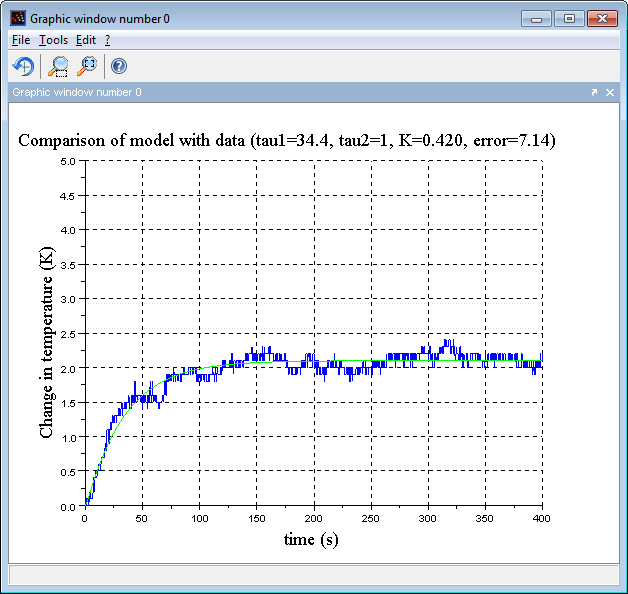
\includegraphics[width=\linewidth]{Step-test_manual/Sorder_fit.png}
\caption{Output of the Scilab code \ttfamily secondorder.sce}
\label{sorder}
\end{figure}

The fit is much better now.  In particular, the initial inflexion is well captured by this second
order transfer function.


\section{Discussion}
We summarize our findings now. For the first order analysis, the gain is 1.7326851 and the 
time constant $\tau$ is 45.739234 seconds. For the second order analysis, the initial inflexion is 
well captured with the two time constants $\tau_1$=34.4, $\tau_2$= 1 and gain = 0.420. Negative steps 
can also be introduced to make the experiment more informative. One need not keep a particular 
input constant. By varying both the inputs, one can imagine it to be like a step varying disturbance signal.
 
\section{Conducting Step Test on SBHS, virtually}
The step by step procedure for conducting an experiment virtually is explained in 
section \ref{vlabsexpt}. 
\begin{enumerate}
 \item Go to {\tt virtual} folder and then {\tt StepTest} directory.
 \item Perform the experiment using {\tt stepc.sce}
 \item Perform first order analysis using {\tt firstorder\_virtual.sce}
 \item Perform second order analysis using {\tt secondorder\_virtual.sce}
\end{enumerate}

The necessary codes are listed in the section \ref{stepcodes}.


\section{Scilab Code}\label{stepcodes}
\begin{code}
\ccaption{label.sci}{\ttfamily label.sci}
\lstinputlisting{Scilab/local/Step_Analysis/Kp-tau-order1/label.sci}
\end{code}

\begin{code}
\ccaption{costf\_1.sci}{\ttfamily costf\_1.sci}
\lstinputlisting{Scilab/local/Step_Analysis/Kp-tau-order1/costf_1.sci}
\end{code}


\begin{code}
\ccaption{firstorder.sce}{\ttfamily firstorder.sce}
\lstinputlisting{Scilab/local/Step_Analysis/Kp-tau-order1/firstorder.sce}
\end{code}

\begin{code}
\ccaption{costf\_2.sci}{\ttfamily costf\_2.sci}
\lstinputlisting{Scilab/local/Step_Analysis/Kp-tau-order2/costf_2.sci}
\end{code}

\begin{code}
\ccaption{order\_2\_heater.sci}{\ttfamily order\_2\_heater.sci}
\lstinputlisting{Scilab/local/Step_Analysis/Kp-tau-order2/order_2_heater.sci}
\end{code}

\begin{code}
\ccaption{secondorder.sce}{\ttfamily secondorder.sce}
\lstinputlisting{Scilab/local/Step_Analysis/Kp-tau-order2/secondorder.sce}
\end{code}

\begin{code}
\ccaption{ser\_init.sce}{\ttfamily ser\_init.sce}
\lstinputlisting{Scilab/local/Step_test/ser_init.sce}
\end{code}

\begin{code}
\ccaption{step\_test.sci}{\ttfamily step\_test.sci}
\lstinputlisting{Scilab/local/Step_test/step_test.sci}
\end{code}

\begin{code}
\ccaption{stepc.sce}{\ttfamily stepc.sce}
\lstinputlisting{Scilab/virtual/StepTest/stepc.sce}
\end{code}

\begin{code}
\ccaption{steptest.sci}{\ttfamily steptest.sci}
\lstinputlisting{Scilab/virtual/StepTest/steptest.sci}
\end{code}

\begin{code}
\ccaption{firstorder\_virtual.sce}{\ttfamily firstorder\_virtual.sce}
\lstinputlisting{Scilab/virtual/Step_Analysis/Kp-tau-order1/firstorder_virtual.sce}
\end{code}

\begin{code}
\ccaption{secondorder\_virtual.sce}{\ttfamily secondorder\_virtual.sce}
\lstinputlisting{Scilab/virtual/Step_Analysis/Kp-tau-order2/secondorder_virtual.sce}
\end{code}












\chapter{Identification of transfer function of a Single Board Heater System through Ramp response experiments}\label{chap2}
The Aim of this experiment is to perform Ramp test on the Single Board Heater System and to identify the system transfer function using Ramp response data. The target group is anyone who has basic knowledge of Control Engineering.
\section{About this Experiment}

\begin{figure}
\centering
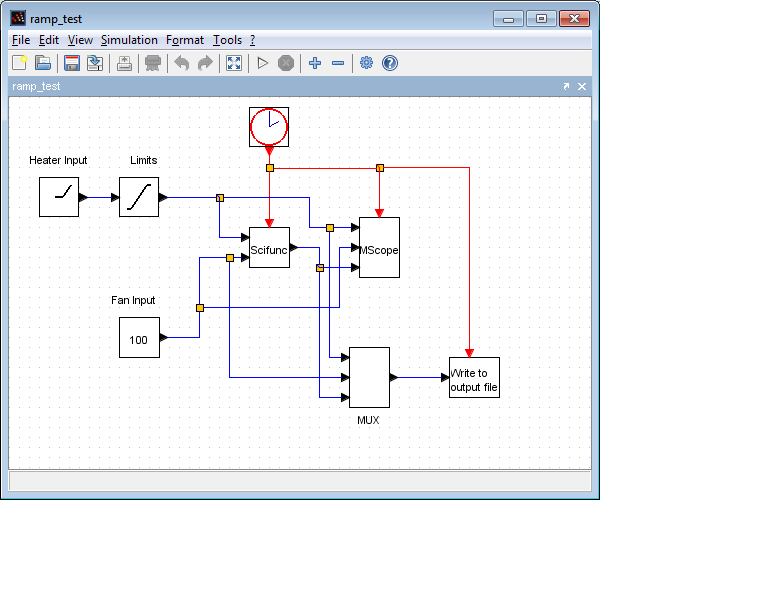
\includegraphics[width=0.7\linewidth]{Ramp-test_manual/ramp_xcos.jpg}
\caption{Xcos for Ramp Test experiment}
\label{Xcos_rt}
\end{figure} 
We have used Scilab-5.2.2 and Xcos for sending and receiving data. This interface is shown in Fig.\ref{Xcos_rt}. Heater current and fan speed are the two inputs to the SBHS system. They are given in PWM units. These inputs can be varied through the Xcos interface by setting the properties of the input blocks in Xcos. The data acquired in the process is stored in the local drive using the "Write to output file" block and is available to the user for further analysis.
\section{Theory}
Identification of the transfer function of a system is quite important since it helps us to model the physical system mathematically. Once the transfer function is obtained one can find out the response of the system, to various inputs, without actually applying them to the system.
Consider the standard first order transfer function given below
\begin{align}
G(s) &= \frac{ C(s)}{ R(s)}\\
G(s)&=\frac K{\tau s+1}\\                           
\intertext{Rewriting the equation by substituting equation 4.2 in equation 4.1, we get}
C(s)  &= K \left\{\frac {R(s)}{\tau s + 1}\right\}\label{fotf}
\intertext{Let us consider the case of giving a ramp input to this first order system. The Laplace Transform of a ramp function with slope = $\upsilonup$ is $ \frac \upsilonup {s^2}$. Substituting $ R(s) = \frac \upsilonup {s^2}$ in equation \ref{fotf}, we obtain}
C(s) & =  \frac K{\tau s + 1}\frac \upsilonup {s^2}\\
&= \frac A{s} + \frac B{s^2} +\frac C{\tau s + 1}\\
\intertext{Solving $C(s)$ using Heaviside expansion approach, we get}
C(s) &= K\upsilonup \left\{\frac1{s^2} -  \frac \tau s + \frac {\tau^2}{\tau s + 1}\right\}\label{Heaviside}\\
\intertext{Taking the Inverse Laplace transform of the above equation, we get}
c(t)&= K\upsilonup \left\{t -\tau   + \tau e^{\frac {-t}\tau }\right\}\label{ct} \\
\intertext{The difference between the reference and output signal is the error signal $e(t)$. Therefore,}
e(t)&= r(t) - c(t)\\
e(t)&= K\upsilonup t - K\upsilonup t + K\upsilonup \tau  - K\upsilonup \tau e^\frac {-t}\tau   \\
e(t)&= K\upsilonup \tau (1 - e^{\frac {-t}\tau})\label{et}\\
\intertext{Normalizing equation \ref{et} for $t>>\tau$, we get}
e(t) &= \tau
\end{align}
This means that the error in following the ramp input is equal to $\tau$ for large value of $t$ \cite{ogt05}. Hence, the smaller the time constant $\tau$ , the smaller is the steady state error.
\section{Step by step procedure to perform Ramp Test}
Change the scilab working directory to {\tt Ramp\_Test} folder. Execute the code {\tt ser\_init.sce} and {\tt ramp\_test.sci}. Open the Xcos code {\tt ramp\_test.xcos}. Give a ramp input to the system with some value for slope. For this experiment, we have chosen $slope = 0.1$. Double click on the ramp input block labled as "Heater input". Put the following values in the respective fields. Slope = 0.1, start time = 300, initial output = 20. Keep the fan constant at 100. Note that the value of heater current will not exceed 40 PWM units due to the use of limit blocks. Running the xcos code may warn you with a message saying "No continuous-time states. Thresholds are ignored". Ignore the message by clicking on OK button.
\begin{figure}
\centering
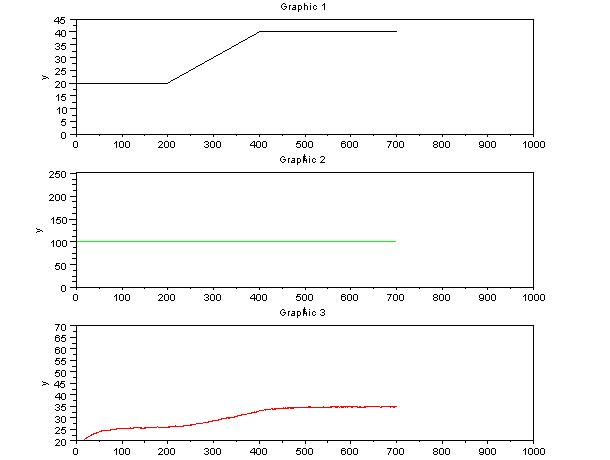
\includegraphics[width=\linewidth]{Ramp-test_manual/ramp_plot.jpg}
\caption{Screen shot of Ramp Test Experiment}
\end{figure}
The data thus obtained is stored using "Write to output file" Xcos block as shown in Fig.\ref{Xcos_rt}.
\begin{table}
\begin{verbatim}
 0.000E+00  0.100E+02  0.100E+03  0.216E+02
 0.100E+00  0.100E+02  0.100E+03  0.216E+02
.
.
 0.251E+03  0.300E+02  0.100E+03  0.291E+02
 0.251E+03  0.300E+02  0.100E+03  0.291E+02
\end{verbatim}
\caption{Ramp data obtained after performing the Ramp Test}
\label{Rampdata}
\end{table}
The first column of Table \ref{Rampdata} denotes time in seconds. The second column denotes heater current. The third column denotes the fan speed. It has been held constant at 100 units. The last column denotes the plate temperature.
\\
\section{Ramp Analysis}
After completing the ramp test experiment, let us do the analysis. Change the directory to {\tt Ramp\_Analysis}. Execute the file {\tt ramp.sce}. On executing this file, you get the values of Kp, tau and Kp approx and tau approx on the Scilab Console Window. You will also get a plot of the ramp response calculated using the equation \ref{ct} for Kp and tau values.
\begin{figure}[h]
	\centering
		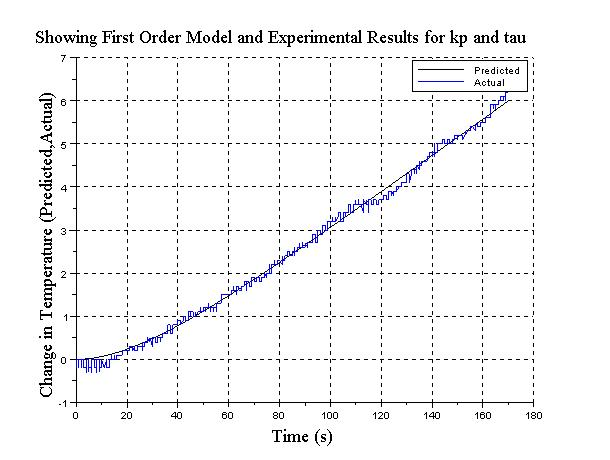
\includegraphics[width=\linewidth]{Ramp-test_manual/fit_curve_ramp.jpg}
	\caption{Ramp response for Kp and tau}
	\label{fig:fit_curve_ramp}
\end{figure}

\section{Discussion}
We summarize our findings now. The experiment has been performed by varying the heater current and keeping the fan speed constant. However, the user is encouraged to try out the experiment using different combinations of fan speed and heater current. Negative ramp can also be tried out to make the experiment more informative. It is not necessary to keep a particular input constant. For example, you can try giving a step input to the disturbance signal, i.e., the fan input. The system can also be treated as a second order system. This consideration is necessary since it increases the accuracy of the acquired transfer function.\cite{kmm09}
\section{Conducting Ramp Test on SBHS, virtually}
The step by step procedure for conducting an experiment virtually is explained in section \ref{vlabsexpt}. The required .sce file is {\tt ramptest.sce}.  You will find this file in the {\tt RampTest} directory under {\tt virtual} folder. Please note that the analysis code of ramp test data obtained by a virtual experiment is slightly different. The procedure to use the analysis code however remains the same as explained earlier. To do a first order analysis, one has to use the file {\tt firstorder\_virtual.sce}. These files are available in the {\tt Ramp\_Analysis} folder under the {\tt virtual} folder. The necessary codes are listed in the section \ref{rampcodes}.

\section{Scilab Code}\label{rampcodes}
\begin{code}
\ccaption{ramp\_test.sci}{\ttfamily ramp\_test.sci}
\lstinputlisting{Scilab/local/Ramp_Test/ramp_test.sci}
\end{code}

\begin{code}
\ccaption{label.sci}{\ttfamily label.sci}
\lstinputlisting{Scilab/local/Ramp_Analysis/label.sci}
\end{code}

\begin{code}
\ccaption{cost.sci}{\ttfamily cost.sci}
\lstinputlisting{Scilab/local/Ramp_Analysis/cost.sci}
\end{code}

\begin{code}
\ccaption{cost\_approx.sci}{\ttfamily cost\_approx.sci}
\lstinputlisting{Scilab/local/Ramp_Analysis/cost_approx.sci}
\end{code}

\begin{code}
\ccaption{ramptest.sci}{\ttfamily ramptest.sci}
\lstinputlisting{Scilab/virtual/RampTest/ramptest.sci}
\end{code}

\begin{code}
\ccaption{ramptest.sce}{\ttfamily ramptest.sce}
\lstinputlisting{Scilab/virtual/RampTest/ramptest.sce}
\end{code}

\begin{code}
\ccaption{ramp\_virtual.sce}{\ttfamily ramp\_virtual.sce}
\lstinputlisting{Scilab/virtual/Ramp_Analysis/ramp_virtual.sce}
\end{code}


%\bibliography{New} % Adding References

\chapter{Frequency Response Analysis of a Single Board Heater System by the Application of Sine Wave}
The aim of this experiment is to do a frequency response analysis of a Single Board Heater System by the 
application of sine wave. The target group is anyone who has basic knowledge of control engineering.\\
\begin{figure}
\centering
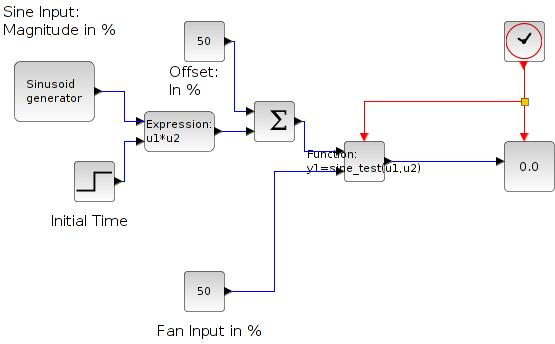
\includegraphics[width=\linewidth]{sinetest_manual/sine_test.jpg}
\caption{Xcos for this experiment}
\label{xcos_sine}
\end{figure}
We have used Scilab with Xcos as an interface for sending and receiving data. 
This interface is shown in figure \ref{xcos_sine}. Heater current and fan speed are the two inputs to the system. 
The heater current is varied sinusoidally. A provision is made to set the parameters related to it like frequency, amplitude 
and offset. The temperature profile thus obtained is the output.\\
In this experiment we are applying a sine change in the heater current by keeping the fan speed constant. 
After application of sine change, wait for sufficient amount of time to allow the temperature to reach a steady-state.
\section{Theory}
 Frequency response of a system means its steady-state response to a sinusoidal input. 
 For obtaining a frequency response of a system, we vary the frequency of the input signal over a spectrum of interest. 
 The analysis is useful and simple because it can be carried out with the available signal generators and measuring devices.\\
Consider a sinusoidal input
\begin{align}
U(t) &= Asin \omega t
\intertext{The Laplace transform of the above equation yields}
U(s) &= \frac{A\omega}{s^2 + \omega^2} \label{lap_tran}
\intertext{Consider the standard first order transfer function given below}
G(s) &= \frac {Y(s)}{U(s)} = \frac K{s + 1}
\intertext{Replacing the value of U(s) from equation \ref{lap_tran}, we get}
Y(s) &= \frac{KA\omega}{(\tau s + 1)(s^2 + \omega ^2)}\\
&=\frac{KA}{\omega ^2\tau ^2 + 1}\left[\frac{\omega \tau ^2}{\tau s +1}- \frac{\tau s \omega}{s^2 + \omega^2}+\frac{\omega}
{s^2 + \omega^2}\right]
\intertext{Taking Laplace Inverse, we get}
y(t) &= \left[\frac {KA}{\omega^2\tau^2+ 1}\right]\left[\omega \tau e^{\frac {-t}{\tau}}-\omega \tau cos(\omega t)+
sin(\omega t)\right] 
\intertext{The above equation has an exponential term $e^\frac{-t}{\tau}$. Hence, for large value of time, its value will 
approach to zero and the equation will yield a pure sine wave. One can also use trigonometric identities to make the equation 
look more simple.}
y(t) &= \left[\frac{KA}{\sqrt{\omega^2 \tau^2 + 1}}\right]\left[sin (\omega t) + \phi \right]
\intertext{where,}
\phi &= -tan^{-1}(\omega \tau)
\intertext{By observing the above equation, one can easily make out that for a sinusoidal input the output is also sinusoidal
but has some phase difference. 
Also, the amplitude of the output signal, $\hat{A}$, has become a function of the input signal frequency, $\omega$.}
\hat{A}&=\frac{KA}{\sqrt{\omega^2 \tau^2 + 1}}
\intertext{The amplitude ratio (AR) can be calculated by dividing both sides by the input signal amplitude A.}
AR &=\frac{\hat{A}}{A}=\frac{K}{\sqrt{\omega^2 \tau^2 + 1}}
\intertext{Dividing the above equation by the process gain K yields the normalized amplitude ratio $(AR_n)$}
AR_n &=\frac{AR}{K}=\frac{1}{\sqrt{\omega^2 \tau^2 + 1}}
\end{align}
Because the process steady state gain is constant, the normalized amplitude ratio is often used for 
frequency response analysis \cite{dale04}.


\section{Procedure to perform Sine Test}
Follow the procedure explained in section \ref{scilab_sbhs}.
\begin{enumerate}
 \item Change the current working directory of Scilab to the folder {\tt Sine\_Test}. 
 \item Execute the code {\tt sinetest.sce} and {\tt sinetest.sci}.
 \item Open the Xcos file {\tt sine\_test.xcos}. 
 \item Initiate a sine input to the system by setting sinusoid generator block properties with some value of the frequency  
($0.007Hz$) and amplitude ($10$).
\end{enumerate}
Note that at high frequencies the plant output is not sinusoidal, which is not of any use. 
Hence, avoid choosing frequencies above $0.04Hz$.

\begin{figure}
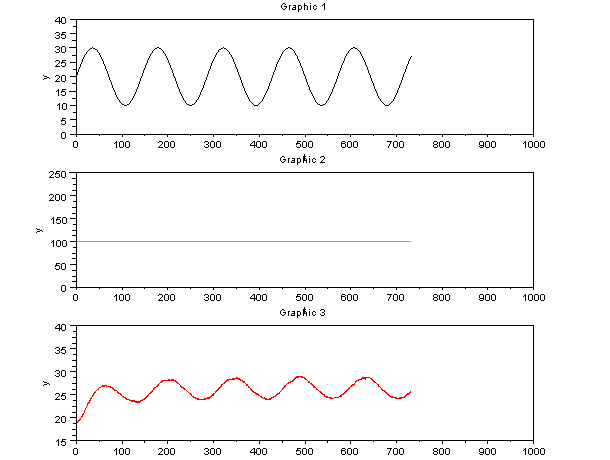
\includegraphics[width=\linewidth]{sinetest_manual/sine_resp.png}
\caption{Plot for sine input 0.007Hz}
\label{fig:scope}
\end{figure}
\begin{table}

\begin{verbatim}
 0.100E+00  0.200E+02  0.100E+03  0.239E+02
 0.200E+00  0.201E+02  0.100E+03  0.238E+02
 0.300E+00  0.201E+02  0.100E+03  0.238E+02
.
.
.
 0.749E+03  0.300E+02  0.100E+03  0.301E+02
 0.749E+03  0.300E+02  0.100E+03  0.302E+02
 0.749E+03  0.300E+02  0.100E+03  0.302E+02
\end{verbatim}
\caption{Data obtained after application of sine input of $0.04Hz$}
\label{sine_data}
\end{table}
The sine test data file is shown in table \ref{sine_data}. Refering to table \ref{sine_data} the first column represents samples. 
The second column represents heater in percentage. Here, it is sinusoidally varied. 
The third column represents fan in percentage. Note that its value is 100 throughout the experiment. 
The fourth column represents the output temperature.
It should be taken into consideration that all the values mentioned in the data file are in percentage of maximum output,
except for the temperature which is in \textcelsius. 

\section{Sine Test Analysis}
Now let us calculate amplitude ratio and phase difference. 
\begin{enumerate}
 \item Change the current working directory of Scilab to the 
folder {\tt Sine\_Analysis}.
\item Copy the data files generated after the completion of the experiment into the 
{\tt Sine\_Analysis} folder.
\item Place the arguments {\ttfamily f} and {\ttfamily filename} in the Scilab code 
{\ttfamily sine2.sce} for the calculation of the above parameters and execute it. Here {\ttfamily f}
means input frequency.
\end{enumerate}

  
\begin{figure}
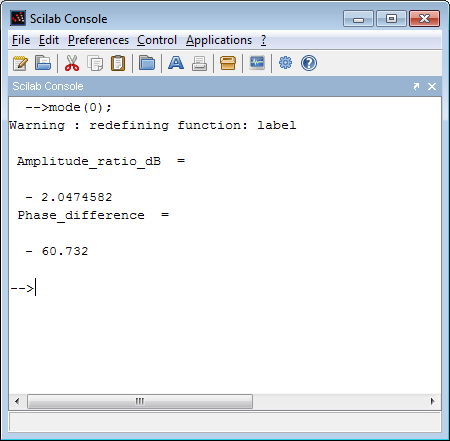
\includegraphics[width=\linewidth]{sinetest_manual/bode_calc.png}
\caption{Scilab Output}
\label{scilab_op}
\end{figure}
It could be seen from figure \ref{scilab_op} that the amplitude r
atio turns out to be $-2.047$dB and phase difference to be $-60.732$\textdegree.
The plot thus obtained is shown in figure \ref{plot0.4}
\begin{figure}
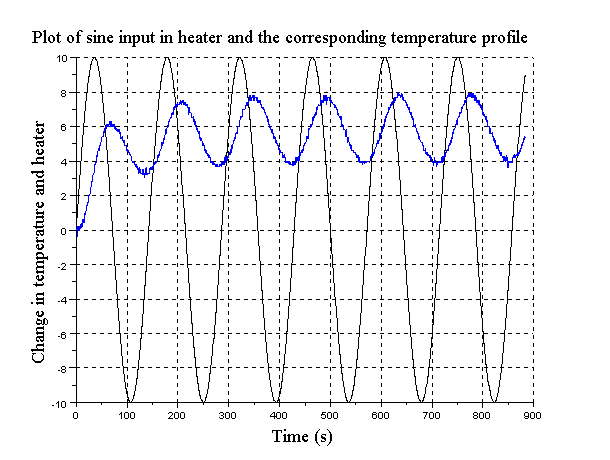
\includegraphics[width=\linewidth]{sinetest_manual/bode_resp}
\caption{Plot of Input and Output vs time}
\label{plot0.4}
\end{figure}

Repeat this calculation over a range of frequencies and note down the values of amplitude ratio in dB and phase difference. 
Input these values for the appropriate frequencies into the Scilab code {\ttfamily TFbode.sce} and execute it to get a 
Bode plot of the plant which is illustrated in figure \ref{bode_plot}.
\begin{figure}
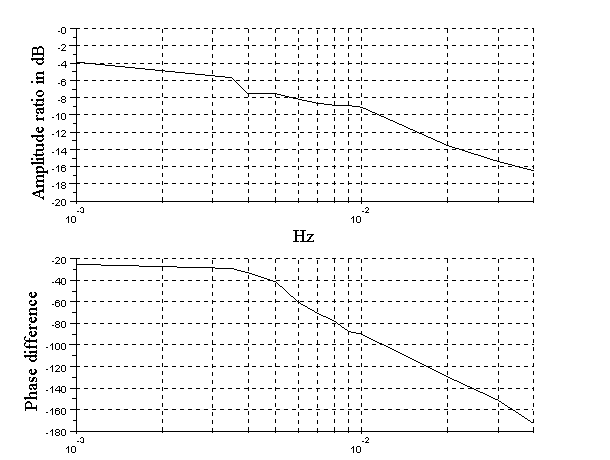
\includegraphics[width=\linewidth]{sinetest_manual/bodeplot}
\caption{Bode plot obtained from the plant}
\label{bode_plot}
\end{figure}

Bode plot can be obtained directly from the plant's second order transfer function \cite{kmm09} with the help of Scilab code
{\ttfamily TFbode.sce}, as shown in figure \ref{tfbode}. A visual comparison of the two Bode plots can be done to 
validate the Bode diagram obtained from the plant.
\begin{figure}
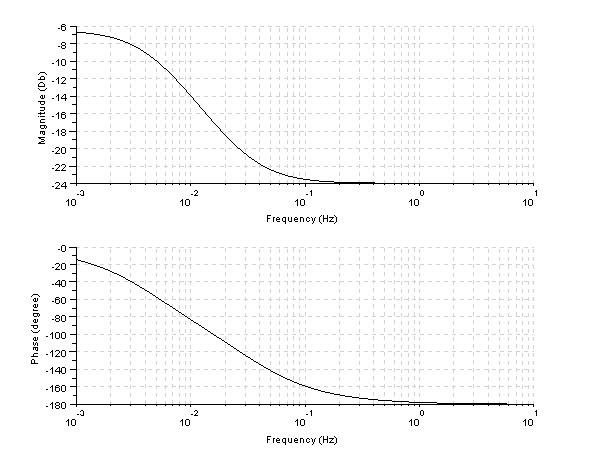
\includegraphics[width=\linewidth]{sinetest_manual/plant_bode_tf}
\caption{Bode plot obtained through plant's transfer function}
\label{tfbode}
\end{figure}

To compare the two plots, we plot it on the same graph as shown in figure \ref{compare_bode}
\begin{figure}
\centering
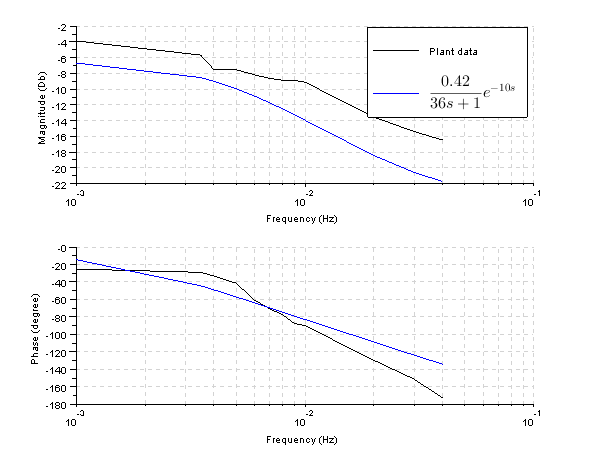
\includegraphics[width=\linewidth]{sinetest_manual/bode_comparison}
\caption{Comparison of Bode plots}
\label{compare_bode}
\end{figure}


\section{Conducting Sine Test on SBHS, virtually}
The step by step procedure for conducting an experiment virtually is explained in section \ref{vlabsexpt}. 
\begin{enumerate}
 \item Go to {\tt virtual} folder and then {\tt SineTest} directory .
 \item Execute {\tt sinetest.sce}.
 \item Perform sine test analysis by executing the file {\tt sine2\_virtual.sce} in {\tt Sine\_Analysis} directory 
 under {\tt virtual} folder.
\end{enumerate}
The necessary codes are listed in the section \ref{sinecodes}.


\section{Scilab Code}\label{sinecodes}

\begin{code}
\ccaption{sine\_test.sci}{\ttfamily sine\_test.sci}
\lstinputlisting{Scilab/local/Sine_Test/sine_test.sci}
\end{code}


\begin{code}
\ccaption{sinetest.sce}{\ttfamily sinetest.sce}
\lstinputlisting{Scilab/virtual/SineTest/sinetest.sce}
\end{code}

\begin{code}
\ccaption{sinetest.sci}{\ttfamily sinetest.sci}
\lstinputlisting{Scilab/virtual/SineTest/sinetest.sci}
\end{code}

\begin{code}
\ccaption{sine2.sce}{\ttfamily sine2.sce}
\lstinputlisting{Scilab/local/Sine_Analysis/sine2.sce}
\end{code}

\begin{code}
\ccaption{lable.sci}{\ttfamily label.sci}
\lstinputlisting{Scilab/local/Sine_Analysis/label.sci}
\end{code}

\begin{code}
\ccaption{bodeplot.sce}{\ttfamily bodeplot.sce}
\lstinputlisting{Scilab/local/Sine_Analysis/bodeplot.sce}
\end{code}


\begin{code}
\ccaption{labelbode.sci}{\ttfamily labelbode.sci}
\lstinputlisting{Scilab/local/Sine_Analysis/labelbode.sci}
\end{code}


\begin{code}
\ccaption{TFbode.sce}{\ttfamily TFbode.sce}
\lstinputlisting{Scilab/local/Sine_Analysis/TFbode.sce}
\end{code}

\begin{code}
\ccaption{comparison.sce}{\ttfamily comparison.sce}
\lstinputlisting{Scilab/local/Sine_Analysis/comparison.sce}
\end{code}

\begin{code}
\ccaption{sine2\_virtual.sce}{\ttfamily sine2\_virtual.sce}
\lstinputlisting{Scilab/virtual/Sine_Analysis/sine2_virtual.sce}
\end{code}



\chapter {Controlling Single Board Heater System using PID controller}
The aim of this experiment is to apply a PID controller to the Single Board Heater System. 
The target group is anyone who has basic knowledge of control engineering.\\
\begin{figure}
\centering
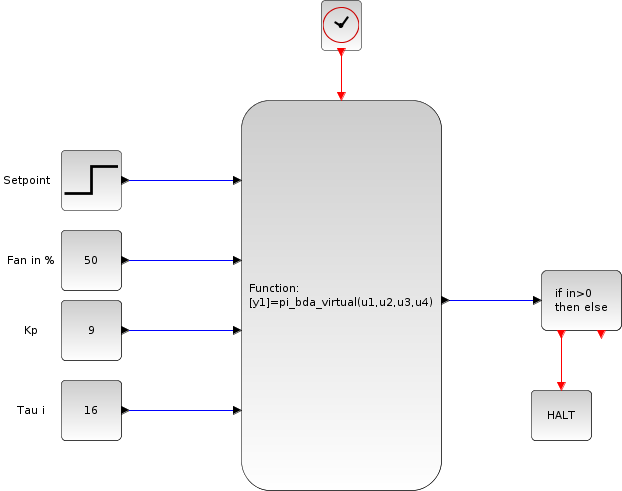
\includegraphics[width=0.7\linewidth]{pid_manual/pid_xcos.png}
\caption{Xcos interface for this experiment}
\label{Xcos_pid}
\end{figure}
Scilab is used with Xcos as an interface for sending and receiving data. 
This interface is shown in figure \ref{Xcos_pid}. Heater current and fan speed are the two inputs to the system. 
The inputs are provided in percentage of maximum output. The parameters related to PID controller $(K,\tau_i,\tau_d)$ can be set in Xcos. 
In this experiment, the fan speed is kept constant. The output temperature profile, read by the sensor, is also plotted. 
The data acquired in the process is stored on the local drive and is available to the user for further calculations.
\section{Theory}
A PID controller tries to minimize the error between measured variable and the setpoint by calculating the error 
and then taking a suitable corrective action. Note that the output of interest is called the measured variable or process 
variable, the difference between the setpoint and the measured variable is called the error and the control action taken 
to minimize the error is given as input to the process in the form of the manipulated variable. A PID controller does 
not simply add or subtract the error in order to calculate control action but instead uses three distinct control features, 
namely, Proportional, Integral and Derivative. Thus, a PID controller has three separate parameters.
 \subsection{Proportional Control Action}
This parameter generates a control action based on the current value of the error. In a more simplified sense, 
if the error is +2, the control action is  -2. The proportional action can be generated by multiplying the error 
with a proportional constant- $K_p$. Mathematical representation of the same is given below,
\begin{align}
P &= K_p e(t)
\end{align}
where,\\
$P$ is the proportional output\\
$K_p$ is the proportional gain\\
$e(t)$ is the error signal

The value of  $K_p$ is very important. A large value of $K_p$ may lead to instability of the system. In contrast, 
a smaller value of $K_P$ may decrease the controller's sensitivity towards error. The problem involved in using only 
proportional action is that the control action will never settle down to its target value and will always retain 
a steady-state error.
\subsection{Integral Control Action}
This parameter generates a control action depending on the history of errors. It means that the action is based on 
the sum of the recent errors. It is proportional to both the magnitude as well as duration of the error. The summation
of the error over a period of time gives a value of the offset that should have been corrected previously. The integral 
action can thus be generated by multiplying this accumulated error with an integral gain $K_i$. Mathematical representation 
of the same is given below.
\begin{align}
I&=K_i\int_0^te(t)dt
\end{align}
where,\\
$I$ is the integral output\\
$K_i$ is the integral gain ($K_i=K_p / \tau _i$, where, $\tau _i$ is the integral time)

The integral action tends to accelerate the control action. However, since it looks only at the past values of the error, 
there is always a possibility of it causing the present values to overshoot the setpoint values.

\subsection{Derivative Control Action}
As the name suggests, a derivative parameter generates a control action by calculating the rate of change of error. 
A derivative action is thus generated by multiplying the value of rate of change of error with a derivative gain $K_d$. 
Mathematical representation of the same is given below.
\begin{align}
D&=K_d\frac{d}{dt}e(t)
\end{align}
where,\\
$D$ is the derivative output\\
$K_d$ is the derivative gain ($K_d=K_p / \tau _d$, where, $\tau _d$ is the derivative time)

The derivative action slows down the rate of change of the controller output. A derivative controller is quite useful when 
the error is continuously changing with time. One should, however, avoid using it alone. This is because there is no output 
when the  error is zero and when the rate of change of error is constant.
\\
When all the above control actions are summed up and used together, the final equation becomes
\begin{align}
PID&=K_pe(t)+K_i\int_0^t e(t)dt+K_d\frac{d}{dt}e(t)
\end{align}
The above equation represents an ideal form of PID controller. This means that the integral controller can be used 
independently. However, it is not a good decision since, the integral action begins only after the error exits for 
some amount of time. The proportional controller however begins as soon as the error starts existing. Hence, the integral 
controller is often used in conjunction with a proportional controller. This is popularly known as PI controller and the
equation for Proportional Integral action becomes,
\begin{align}
PI&=K_pe(t)+\left(K_p/\tau _i\right)\int_0^te(t)dt\\
&=K_p\left\{e(t)+\left(1/\tau _i\right)\int_0^te(t)dt\right\}
\end{align}
Similarly, as discussed before, independent use of derivative controller is also not desirable. Moreover, if the process 
contains high frequency noise then the derivative action will tend to amplify the noise. Hence, derivative controller is 
also used in conjunction with Proportional or Proportional Integral controller popularly known as PD or PID, respectively. 
Therefore the equation for Proportional Derivative action becomes,
\begin{align}
PD&=K_pe(t)+K_p\tau _d\frac{d}{dt}e(t)\\
&=K_p\left\{e(t)+\tau _d\frac{d}{dt}e(t)\right\}
\intertext{Finally, writing the equation for PID controller,}
PID&=K\left\{e(t)+\frac 1{\tau _i}\int_0^te(t)dt+\tau _d\frac{d}{dt}e(t)\right\}\label{pid}
\end{align}
\section{Ziegler-Nichols Rule for Tuning PID Controllers}
There are many rules to tune a PID controller. We shall see the two popular methods suggested by Ziegler-Nichols.
\subsection{First Method}
\begin{figure}
\centering
\includegraphics[width=\linewidth]{pid_manual/ReacCurve}
\caption{Reaction curve \cite{kmmdc09}}
\label{RC}
\end{figure}
Ziegler-Nichols rule determines the values of gain $K$, integral time $\tau_i$ and derivative time $\tau_d$ based on 
the step response characteristics of a given plant. In this method, one can experimentally obtain the response of a plant 
to a step input, as shown in figure \ref{RC}. This method is applicable only when the response to the step input exhibits 
S-shaped curve \cite{ogt05}.\\
As shown in figure \ref{RC}, by drawing the tangent line at the inflection point and determining the intersection of the 
tangent line with the time axis and the line $c(t)= K$ ,we get two constants, namely, delay time $L$ and time constant $T$.

Ziegler and Nichols suggested to set the values of $K, \tau_i , \tau_d$  according to the formula shown in table \ref{table}.
\begin{table}
\begin{center}
\renewcommand{\arraystretch}{1.5}
\begin{tabular}{|c|r|r|r|}\hline
Type of
controller & $K$ & $\tau_i$ & $\tau_d$ \\ \hline
$P$ & $\frac{1}{RL}$ & $\infty$ & 0 \\ \hline
$PI$ & $\frac{0.9}{RL}$ & $3L$ & 0 \\\hline
$PID$ & $\frac{1.2}{RL}$ & $2L$ & $0.5L$ \\ \hline
\end{tabular}
\caption{Ziegler-Nichols tuning rule based on step response of plant}
\label{table}
\end{center}
\end{table}
Notice that the PID controller tuned by the Ziegler-Nichols rule gives,
\begin{align}
G_c(s)&=K_p\left(1+\frac 1{T_is}+T_ds\right)\\
&=1.2\frac {T}{L}\left( 1+\frac 1{2Ls}+0.5Ls\right)\\
&=0.6T\frac{\left(s+\frac 1{L}\right)^2}{s}
\end{align}
Thus, the PID controller has a pole at the origin and double zeros at $s= -1/L$.

\subsection{Second Method}
\begin{figure}
\centering
\includegraphics[width=\linewidth]{pid_manual/PIDUGtune}
\caption{Ziegler-Nichols instability tuning method}
\label{instability}
\end{figure}

The second method is also known as \textquoteleft instability method \textquoteright \cite{kmm09}. This is a closed 
loop method in which the integral and derivative gains of the PID controller are made zero with a unity value for 
proportional gain. A setpoint change is made and the temperature profile is observed for some time. The temperature 
would most likely maintain a steady-state with some offset. The gain is increased to a next distinct value (say 2) 
with a change in the setpoint. The procedure is repeated until the temperature first varies with sustained oscillations. 
It is necessary that the output (temperature) should have neither under damped nor over damped oscillations. At this 
particular frequency of sustained oscillations, the corresponding value of $K_p$ is noted and is called as the critical
gain $K_{cr}$. The corresponding period of oscillation is known as  $P_{cr}$. Refer to figure \ref{instability}.

The various P, PI and PID parameters are then calculated with the help of table \ref{2ndmtd}.
\begin{table}
\begin{center}
\renewcommand{\arraystretch}{1.5}
\begin{tabular}{|c|r|r|r|}\hline
Type of
controller & $K$ & $\tau_i$ & $\tau_d$ \\ \hline
$P$ & $0.5K_{u}$ & $\infty$ & 0 \\ \hline
$PI$ & $0.45K_{u}$ & $\frac{1}{0.2}P_{u}$ & 0 \\\hline
$PID$ & $0.6K_{u}$ & $0.5P_{u}$ & $0.125P_{u}$ \\ \hline
\end{tabular}
\caption{Ziegler-Nichols tuning rule for instability tuning method}
\label{2ndmtd}
\end{center}
\end{table}
Using the Ziegler-Nichols method explained earlier, the following values were obtained. Refer to figure \ref{steptest}.

\begin{figure}
\centering
\includegraphics[width=0.7\linewidth]{pid_manual/forder_fit}
\caption{Refer to \textquoteleft Step Test\textquoteright experiment \cite{kmm09}}
\label{steptest}
\end{figure}
\begin{align*}
L&=6\hspace{0.2cm}s\\
T&=193\hspace{0.2cm}s
\intertext{For PI}
K&=6.031\\
\tau _i&= 18\hspace{0.25cm}
\intertext{For PID}
K&=8\\
\tau _i&= 12\hspace{0.25cm}\\
\tau _d&= 3\hspace{0.25cm}
\end{align*}
While performing the experiment, fine tunning of $K,\tau_i,\tau_d$ may be required.\\

\section{Implementing PI Controller using Trapezoidal Approximation}
Figure \ref{pi_cos} shows Xcos diagram for implementing PI controller.
\begin{figure}
\centering
\includegraphics[width=0.7\linewidth]{pid_manual/pi_ta_xcos.png}
\caption{Xcos for PI controller available as {\tt pi\_ta\_virtual.xcos}}
\label{pi_cos}
\end{figure}
The PI controller in continuous time is given by, 
\begin{align}
u(t)&=K \left\{e(t)+\frac{1}{\tau_i}\int_0^t e(t)dt\right\}
\intertext {On taking the Laplace transform,we obtain}
u(t)&=K\left\{1+\frac 1{\tau_i s}\right\}e(t) \label{lt1}
\intertext{By mapping controller given in equation \ref{lt1} to the discrete time domain using trapezoidal approximation}
u(n)&=K\left\{1+\frac{T_s}{2\tau_i}\frac{z+1}{z-1}\right\}e(n)
\intertext{On cross multiplying, we obtain}
(z-1)u(n)&=K\left\{(z-1)+\frac{T_s}{2\tau_i}(z+1)\right\}e(n)
\intertext{We divide by $z$ and then by using shifting theorem, we obtain}
u(n)-u(n-1)&=K\left\{e(n)-e(n-1)+\frac{T_s}{2\tau_i}e(n)+\frac{T_s}{2\tau_i}e(n-1)\right\}
\intertext{The PI controller is usually written as}
u(n)&=u(n-1)+s_0 e(n)+s_1e(n-1)
\intertext{where}
s_0&=K\left(1+\frac{T_s}{2\tau_i}\right) \\
s_1&=K\left(-1+\frac{T_s}{2\tau_i}\right)
\end{align}

For implementing the PI controller, please follow the steps illustrated in section \ref{scilab_sbhs} of this document with the following changes:
\begin{enumerate}

\item In step 1, change the directory to the folder {\tt pid\_controller} instead of {\tt StepTest}.
\item In step 5, execute the file {\tt pi\_ta.sci} instead of {\tt step\_test.sci}.
\item In step 6, execute the file {\tt pi\_ta.xcos} instead of {\tt step\_test.xcos}.

\end{enumerate}

The output of Xcos is shown in figure \ref{pi_ta}.
Figure shows three plots. First sub plot shows setpoint and output temperature profile. Second sub plot shows 
control effort and third sub plot shows error between setpoint and plant output.

\subsection{Implementing PI controller using Trapezoidal Approximation on SBHS, virtually}


For implementing above PI controller virtually, please follow the steps illustrated in section \ref{vlabsexpt} of this 
document with the following changes:
\begin{enumerate}

\item In step 1, change the directory to the folder {\tt pid\_controller} instead of {\tt StepTest}.
\item In step 5, execute the file {\tt pi\_ta\_virtual.sce} instead of {\tt step\_test.sce}.
\item In step 6, execute the file {\tt pi\_ta\_virtual.xcos} instead of {\tt step\_test.xcos}.

\end{enumerate}



\begin{figure}
\centering
\includegraphics[width=0.6\linewidth]{pid_manual/pi_ta}
\caption{PI controller (Trapezoidal Approximation) output}
\label{pi_ta}
\end{figure}
 
\section{Implementing PI Controller using Backward Difference Approximation}
The PI controller in continuous time is given by 
\begin{align}
u(t)&=K \left\{e(t)+\frac{1}{\tau_i}\int_0^t e(t)dt\right\}
\intertext {On taking the Laplace transform, we obtain}
u(t)&=K\left\{1+\frac 1{\tau_i s}\right\}e(t) \label{lt2}
\intertext{By mapping controller given in equation \ref{lt2} to the discrete time domain using Backward difference 
approximation:}
u(n)&=K\left\{1+\frac{T_s}{\tau_i}\frac{z}{z-1}\right\}e(n)
\intertext{On cross multiplying, we get}
(z-1)u(n)&=K\left\{(z-1)+\frac{T_s}{\tau_i}(z)\right\}e(n)
\intertext{We divide by $z$ and then by using shifting theorem, we obtain}
u(n)-u(n-1)&=K\left\{e(n)-e(n-1)+\frac{T_s}{\tau_i}e(n)\right\}
\intertext{The PI controller is usually written as}
u(n)&=u(n-1)+s_0 e(n)+s_1e(n-1)
\intertext{where}
s_0&=K\left(1+\frac{T_s}{\tau_i}\right) \\
s_1&=-K
\end{align}

For implementing the PI controller,  please follow the steps illustrated in section \ref{scilab_sbhs} of this document with the 
following changes:
\begin{enumerate}

\item In step 1, change the directory to the folder {\tt pid\_controller} instead of {\tt StepTest}.
\item In step 5, execute the file {\tt pi\_bda.sci} instead of {\tt step\_test.sci}.
\item In step 6, execute the file {\tt pi\_bda.xcos} instead of {\tt step\_test.xcos}.

\end{enumerate}

The Xcos output is shown in figure \ref{pi_bda}.
Figure shows three plots. First sub plot shows setpoint and output temperature profile. 
Second sub plot shows control effort and third sub plot shows error between setpoint and plant output.


\begin{figure}
\centering
\includegraphics[width=0.6\linewidth]{pid_manual/pi_bda.jpg}
\caption{PI controller (Backward Difference Approximation) output}
\label{pi_bda}
\end{figure}


\subsection{Implementing PI Controller using Backward Difference Approximation on SBHS, virtually}
For implementing above PI controller virtually, please follow the steps illustrated in section \ref{vlabsexpt} 
of this document with the following changes:
\begin{enumerate}

\item In step 1, change the directory to the folder {\tt pid\_controller} instead of {\tt StepTest}.
\item In step 5, execute the file {\tt pi\_bda\_virtual.sce} instead of {\tt step\_test.sce}.
\item In step 6, execute the file {\tt pi\_bda\_virtual.xcos} instead of {\tt step\_test.xcos}.

\end{enumerate}


\section{Implementing PI Controller using Forward Difference Approximation}
The PI controller in continuous time is given by 
\begin{align}
u(t)&=K \left\{e(t)+\frac{1}{\tau_i}\int_0^t e(t)dt\right\}
\intertext {On taking the Laplace transform, we obtain}
u(t)&=K\left\{1+\frac 1{\tau_i s}\right\}e(t) \label{lt3}
\intertext{By mapping controller given in equation \ref{lt3} to the discrete time domain using forward difference formula, we get}
u(n)&=K\left\{1+\frac{T_s}{\tau_i}\frac{1}{z-1}\right\}e(n)
\intertext{On cross multiplying, we get}
(z-1)u(n)&=K\left\{(z-1)+\frac{T_s}{\tau_i}\right\}e(n)
\intertext{We divide by $z$ and then by using shifting theorem, we get}
u(n)-u(n-1)&=K\left\{e(n)-e(n-1)+\frac{T_s}{\tau_i}e(n-1)\right\}
\intertext{The PI controller is usually written as}
u(n)&=u(n-1)+s_0 e(n)+s_1e(n-1)
\intertext{where}
s_0&=K \\
s_1&=K\left(-1+\frac{T_s}{\tau_i}\right)
\end{align}

For implementing the PI controller, please follow the steps illustrated in section \ref{scilab_sbhs} of this document with the 
following changes:
\begin{enumerate}

\item In step 1, change the directory to the folder {\tt pid\_controller} instead of {\tt StepTest}.
\item In step 5, execute the file {\tt pi\_fda.sci} instead of {\tt step\_test.sci}.
\item In step 6, execute the file {\tt pi\_fda.xcos} instead of {\tt step\_test.xcos}.

\end{enumerate}

The Xcos output is shown in figure \ref{pi_fda}.
Figure shows three plots. First sub plot shows setpoint and output temperature profile. Second sub plot shows 
control effort and third sub plot shows error between setpoint and plant output.

\begin{figure}
\centering
\includegraphics[width=0.6\linewidth]{pid_manual/pi_fda}
\caption{PI controller implementation (Forward Difference Approximation)}
\label{pi_fda}
\end{figure}

\subsection{Implementing PI Controller using Forward Difference Approximation on SBHS, virtually}
For implementing above PI controller virtually, please follow the steps illustrated in section \ref{vlabsexpt} of 
this document with the following changes:
\begin{enumerate}

\item In step 1, change the directory to the folder {\tt pid\_controller} instead of {\tt StepTest}.
\item In step 5, execute the file {\tt pi\_fda\_virtual.sce} instead of {\tt step\_test.sce}.
\item In step 6, execute the file {\tt pi\_fda\_virtual.xcos} instead of {\tt step\_test.xcos}.

\end{enumerate}

\
\section{Implementing PID Controller using Backward Difference Approximation}
Figure \ref{pid_cos} shows Xcos diagram for implementing PID controller.\\
\begin{figure}
\begin{center}
\includegraphics[width=0.6\linewidth]{pid_manual/pid_bda_virtual_xcos.png}
\caption{Xcos for PID controller available as {\tt pid\_bda\_virtual.xcos}}
\label{pid_cos}
\end{center}
\end{figure}

The PID controller in continuous time is given by 
\begin{align}
u(t)&=K \left\{e(t)+\frac{1}{\tau_i}\int_0^t e(t)dt+\tau_d\frac{de(t)}{dt}\right\}
\intertext {On taking the Laplace transform, we obtain}
u(t)&=K\left\{1+\frac 1{\tau_i s}+\tau_d s\right\}e(t) \label{lt4}
\intertext{By mapping controller given in equation \ref{lt4} to the discrete time domain using backward difference formula, we get}
u(n)&=K\left\{1+\frac{T_s}{\tau_i}\frac{z}{z-1}+\frac{\tau_d}{T_s}\frac{z-1}{z}\right\}e(n)
\intertext{On cross multiplying, we obtain}
(z^2-z)u(n)&=K\left\{(z^2-z)+\frac{T_s}{\tau_i}z^2+\frac{\tau_d}{T_s}(z-1)^2\right\}e(n)
\intertext{We divide by $z^2$ and by using shifting theorem, we get}
u(n)-u(n-1)&=K\left\{e(n)-e(n-1)+\frac{T_s}{\tau_i}e(n)\right.\nonumber \\
\hspace{1cm}&+ \left. \frac{\tau_d}{T_s}[e(n)-2e(n-1)+e(n-2)]\right\}
\intertext{The PID controller is usually written as}
u(n)&=u(n-1)+s_0 e(n)+s_1e(n-1)+s_2e(n-2)
\intertext{where}
s_0&=K\left[1+\frac{T_s}{\tau_i}+\frac{\tau_d}{T_s}\right] \\
s_1&=K\left[-1-2\frac{\tau_d}{T_s}\right]\\
s_2&=K\left[\frac{\tau_d}{T_s}\right]
\end{align}

For implementing the PID controller, please follow the steps illustrated in section \ref{scilab_sbhs} of this document with the 
following changes:
\begin{enumerate}

\item In step 1, change the directory to the folder {\tt pid\_controller} instead of {\tt StepTest}.
\item In step 5, execute the file {\tt pid\_bda.sci} instead of {\tt step\_test.sci}.
\item In step 6, execute the file {\tt pid\_bda.xcos} instead of {\tt step\_test.xcos}.

\end{enumerate}

The output of Xcos is shown in figure \ref{pid_bda}.
Figure shows three plots. First sub plot shows setpoint and output temperature profile. Second sub plot shows 
control effort and third sub plot shows error between setpoint and plant output.


\begin{figure}
\centering
\includegraphics[width=0.7\linewidth]{pid_manual/pid_bda_graph}
\caption{PID controller (Backward Difference Approximation) output}
\label{pid_bda}
\end{figure}


\subsection{Implementing PID Controller using Backward Difference Approximation on SBHS, virtually}
For implementing above PI controller virtually, please follow the steps illustrated in section \ref{vlabsexpt} of this 
document with the following changes:
\begin{enumerate}

\item In step 1, change the directory to the folder {\tt pid\_controller} instead of {\tt StepTest}.
\item In step 5, execute the file {\tt pid\_bda\_virtual.sce} instead of {\tt step\_test.sce}.
\item In step 6, execute the file {\tt pid\_bda\_virtual.xcos} instead of {\tt step\_test.xcos}.

\end{enumerate}


\section{Implementing PID Controller using Trapezoidal Approximation for Integral Mode and Backward Difference Approximation 
for the Derivative Mode}
The PID controller in continuous time is given by 
\begin{align}
u(t)&=K \left\{e(t)+\frac{1}{\tau_i}\int_0^t e(t)dt+\tau_d\frac{de(t)}{dt}\right\}
\intertext {On taking the Laplace transform, we obtain}
u(t)&=K\left\{1+\frac 1{\tau_i s}+\tau_d s\right\}e(t) \label{lt5}
\intertext{By mapping controller given in equation \ref{lt5} to the discrete time domain using trapezoidal approximation 
for integral mode and backward difference approximation for the derivative mode, we get}
u(n)&=K\left\{1+\frac{T_s}{2\tau_i}\frac{z+1}{z-1}+\frac{\tau_d}{T_s}\frac{z-1}{z}\right\}e(n)
\intertext{On cross multiplying, we obtain}
(z^2-z)u(n)&=K\left\{(z^2-z)+\frac{T_s}{2\tau_i}(z^2+z)\frac{\tau_d}{T_s}(z-1)^2\right\}e(n)
\intertext{We divide by $z^2$ and then by using shifting theorem, we get}
u(n)-u(n-1)&=K\left\{e(n)-e(n-1)+\frac{T_s}{2\tau_i}{e(n)+e(n-1)}\right.\nonumber \\
\hspace{1cm}&+ \left. \frac{\tau_d}{T_s}[e(n)-2e(n-1)+e(n-2)]\right\}
\intertext{The PID controller is usually written as}
u(n)&=u(n-1)+s_0 e(n)+s_1e(n-1)+s_2e(n-2)
\intertext{where}
s_0&=K\left[1+\frac{T_s}{2\tau_i}+\frac{\tau_d}{T_s}\right] \\
s_1&=K\left[-1+\frac{T_s}{2\tau_i}-2\frac{\tau_d}{T_s}\right]\\
s_2&=K\frac{\tau_d}{T_s}
\end{align}

For implementing the PID controller, please follow the steps illustrated in section \ref{scilab_sbhs} of this document with the 
following changes:
\begin{enumerate}

\item In step 1, change the directory to the folder {\tt pid\_controller} instead of {\tt StepTest}.
\item In step 5, execute the file {\tt pid\_ta\_bda.sci} instead of {\tt step\_test.sci}.
\item In step 6, execute the file {\tt pid\_ta\_bda.xcos} instead of {\tt step\_test.xcos}.

\end{enumerate}

The Xcos output is shown in figure \ref{pid_ta_bda}.
Figure shows three plots. First sub plot shows setpoint and output temperature profile. Second sub plot shows control 
effort and third sub plot shows error between setpoint and plant output.

\begin{figure}
\centering
\includegraphics[width=0.6\linewidth]{pid_manual/pid_ta_bda_graph.jpg}
\caption{PID controller (TA - BDA) implementation}
\label{pid_ta_bda}
\end{figure}
 

\subsection{Implementing PID Controller using Trapezoidal Approximation for Integral Mode and Backward Difference 
Approximation for the Derivative Mode on SBHS, virtually}
For implementing above PID controller virtually, please follow the steps illustrated in section \ref{vlabsexpt} of this 
document with the following changes:
\begin{enumerate}

\item In step 1, change the directory to the folder {\tt pid\_controller} instead of {\tt StepTest}.
\item In step 5, execute the file {\tt pid\_ta\_bda\_virtual.sce} instead of {\tt step\_test.sce}.
\item In step 6, execute the file {\tt pid\_ta\_bda\_virtual.xcos} instead of {\tt step\_test.xcos}.

\end{enumerate}
Due to the introduction of derivative action, control effort shows lots of fluctuations. By using filtered form of 
PID, we can make derivative mode implementable.


\section{Implementing PID Controller with Filtering using Backward Difference Approximation}
Figure \ref{pid_filter_xcos} shows Xcos diagram for implementing PID controller with filtering.
\begin{figure}
\begin{center}
\includegraphics[width=0.6\linewidth]{pid_manual/pidN_virtual_xcos.png}
\caption{Xcos for PID controller with filtering available as {\tt pidN\_virtual.xcos}}
\label{pid_filter_xcos}
\end{center}
\end{figure}
\begin{align}
\intertext{PID filtered form is given by}
u(t)&=K\left\{1+\frac 1{\tau_i s}+\frac{\tau_d s}{1+\frac{\tau_d s}{N}}\right\}e(t) \label{lt6}
\intertext{where N is large number of the order of 100.}
\intertext{By maping controller given in equation \ref{lt6} to the discrete 
time domain using backward difference formula, we get}
u(n)&=K\left(1+\frac{T_s}{\tau_i}\frac{1}{1-z^{-1}}+\frac{\tau_d (1-z^{-1})}{1+\frac{\tau_d(1-z^{-1})}{N}}\right)e(n)\\
u(n)&=K\left(1+\frac{T_s}{\tau_i}\frac{1}{1-z^{-1}}+\frac{Nr_1(1-z^{-1})}{1+r_1z^{-1}}\right)e(n)
\intertext{where}
r_1&=-\frac{\frac{\tau_d}{N}}{\frac{\tau_d}{N}+T_s}
\intertext{On cross multiplying, we obtain}
(1-z^{-1})(1+r_1 z^{-1})u(n)&=K[(1-z^{-1})(1+r_1 z^{-1})\nonumber\\
&+\frac{T_s}{\tau_i}(1+r_1z^{-1})+\frac{\tau_d}{T_s}(1-z^{-1})^2]e(n)
\intertext{Simplifying and then by using shifting theorem, we obtain}
u(n)+(r_1-1)u(n&-1)\nonumber\\
-r_1u(n&-2)=K\left[1+\frac{T_s}{\tau_i}-Nr_1\right]e(n)\nonumber\\
&+K\left[r_1(1+\frac{T_s}{\tau_i}+2N)-1\right]e(n-1)\nonumber\\
&-K\left[r_1(1+N)\right]e(n-2)\\
\intertext{Hence}
u(n)&=r_1u(n-2)-(r_1-1)u(n-1)\nonumber\\
&+s_0 e(n)+s_1e(n-1)+s_2e(n-2)
\intertext{where}
s_0&=K\left[1+\frac{T_s}{\tau_i}-Nr_1\right] \\
s_1&=K\left[r_1(1+\frac{T_s}{\tau_i}+2N)-1\right]\\
s_2&=-K\left[r_1(1+N)\right]
\end{align}

For implementing the PID controller, please follow the steps illustrated in section \ref{scilab_sbhs} of this document with 
the following changes:
\begin{enumerate}

\item In step 1, change the directory to the folder {\tt pid\_controller} instead of {\tt StepTest}.
\item In step 5, execute the file {\tt pid\_filter.sci} instead of {\tt step\_test.sci}.
\item In step 6, execute the file {\tt pidN.xcos} instead of {\tt step\_test.xcos}.

\end{enumerate}

The Xcos output is shown in figure \ref{pid_filter}.
Figure shows three plots. First sub plot shows setpoint and output temperature profile. Second sub plot shows control
effort and third sub plot shows error between setpoint and plant output.

\begin{figure}
\centering
\includegraphics[width=0.7\linewidth]{pid_manual/pid_filter.jpg}
\caption{PID controller (with filtering) implementation}
\label{pid_filter}
\end{figure}

By comparing figure \ref{pid_bda} and figure \ref{pid_filter}, it is clear that introduction of filtered form of 
PID reduces fluctuations in control effort.

\subsection{Implementing PID Controller with Filtering using Backward Difference Approximation on SBHS, virtually}
For implementing the PID controller virtually, please follow the steps illustrated in section \ref{vlabsexpt} of this 
document with the following changes:
\begin{enumerate}

\item In step 1, change the directory to the folder {\tt pid\_controller} instead of {\tt StepTest}.
\item In step 5, execute the file {\tt pid\_filter\_virtual.sce} instead of {\tt step\_test.sce}.
\item In step 6, execute the file {\tt pidN\_virtual.xcos} instead of {\tt step\_test.xcos}.

\end{enumerate}


\section{Scilab Code}\label{pidcodes}
\subsection{Scilab code for serial communication}
%\addtocontents{cod}{\protect\addvspace{\codclr}}
\begin{code}
\ccaption{ser\_init.sci}{ser\_init.sci used for serial communication}
\lstinputlisting{Scilab/local/pid_controller/ser_init.sce}
\end{code}
\subsection{Scilab code for PI controller}
\begin{code}
\ccaption{pi\_ta.sci}{pi\_ta.sci}
\lstinputlisting{Scilab/local/pid_controller/pi_ta.sci}
\end{code}
\begin{code}
\ccaption{pi\_bda.sci}{ pi\_bda.sci}
\lstinputlisting{Scilab/local/pid_controller/pi_bda.sci}
\end{code}
\begin{code}
\ccaption{pi\_fda.sci}{ pi\_fda.sci}
\lstinputlisting{Scilab/local/pid_controller/pi_fda.sci}
\end{code}
\subsection {Scilab code for PID controller}
\begin{code}
\ccaption{pid\_bda.sci}{ pid\_bda.sci}
\lstinputlisting{Scilab/local/pid_controller/pid_bda.sci}
\end{code}
\begin{code}
\ccaption{pid\_ta\_bda.sci}{ pid\_ta\_bda.sci}
\lstinputlisting{Scilab/local/pid_controller/pid_ta_bda.sci}
\end{code}
\begin{code}
\ccaption{pid\_filter.sci}{ pid\_filter.sci}
\lstinputlisting{Scilab/local/pid_controller/pid_filter.sci}
\end{code}

\begin{code}
\ccaption{pid\_bda\_virtual.sce}{pid\_bda\_virtual.sce}
\lstinputlisting{Scilab/virtual/pid_controller/pid_bda_virtual.sce}
\end{code}

\begin{code}
\ccaption{pid\_bda\_virtual.sci}{pid\_bda\_virtual.sci}
\lstinputlisting{Scilab/virtual/pid_controller/pid_bda_virtual.sci}
\end{code}

%\bibliography{pid}

\chapter{Implementing \textquoteleft Two Degrees of Freedom\textquoteright Controller for First order systems on a
Single Board Heater System}
The aim of this experiment is to implement a 2DOF controller on a
single board heater system.  The target group is anyone who has basic
knowledge of Control Engineering.
\begin{figure}
\centering
\includegraphics[width=0.9\linewidth]{2-DOF_manual/2dof_xcos.png}
\caption{Xcos interface for this experiment}
\label{Xcos_2dof}
\end{figure}
We have used Scilab with Xcos as an interface for sending and receiving data. This interface is shown in Fig.\ref{Xcos_2dof}. Fan speed and Heater current are the two inputs to the system. For this experiment, the heater current is used as a control effort generated by inputting the various 2-DOF controller parameters like Rc, Sc, Tc and gamma. The fan input could be thought of as an external disturbance.
\section{Theory}
 Degree of freedom as far as the control theory is concerned is the number of parameters on which the plant is no more dependent or the number of parameters that are free to vary. This means that a higher degree of freedom controller makes the plant less susceptible to disturbances. 
Controllers are broadly classified as feedback and feed forward controllers. Feedback controllers are further classified as One Degree of Freedom controller and Two Degree of Freedom controller. Feed forward controllers are those who take the control action before a disturbance disturbs the plant. But this implies an ability to sense the disturbance. Moreover, exact knowledge about the plant is also needed. Nevertheless, due to these restrictions, it is rarely used alone.
A feedback control strategy is as shown in figure \ref{fb}. The reference and the output is continuously compared to generate error which is fed to the controller to take the appropriate control action. Here, exact knowledge about the plant, $G(z)$ and the disturbance, $v$ is not necessary.
\begin{figure}
\begin{center}
\begin{tikzpicture}[auto, node distance=2cm]
\node[input, name=input]{};
\node[sum,right of=input](sum){};
\draw[->](input) -- node{$r$}(sum);
\node[block, right of=sum](gc){$G_c(z)$};
\draw[->](sum)--node{$e$}(gc);
\node[block, right of=gc, node distance=3cm](g){$G(z)$};
\draw[->](gc)--node{$u$}(g);
\node[sum, right of=g,pin={[pinstyle] above:$v$},node distance=2cm](sum2){};
\draw[->](g)--node{}(sum2);
\node[output,right of=sum2,node distance=1cm](output){};
\draw[->](sum2)--node[name=y]{$y$}(output);
\draw [->] (y)--(8.58,-1.5)-|(sum)node[pos=0.88] {$-$};
\end{tikzpicture}
\end{center}
\caption{Feed back control strategy}
\label{fb}
\end{figure}

Solving for y(n), we get
\begin{align}
y(n)&=\frac{G(z)G_c(z)}{1+G(z)G_c(z)}r(n)+\frac 1{1+G(z)G_c(z)}v(n)
\intertext{let,}
T(z)&=\frac{G(z)G_c(z)}{1+G(z)G_c(z)}\\
S(z)&=\frac 1{1+G(z)G_c(z)}
\intertext{this implies}
y(n)&=T(z)r(n)+S(z)v(n)
\intertext{Here it could be seen that the controller has to track the reference input as well as eliminate the effect of external disturbance. But, however from the above equation it could be seen that}
S + T &= 1
\end{align}
Hence it is not possible to achieve both of the requirements, simultaneously in this particular control arrangement. This control arrangement is called {\ttfamily One Degree of Freedom}, abbreviated as 1-DOF.
A {\ttfamily Two Degrees of Freedom} strategy is as shown in figure \ref{2dof}. Here, $G_b$ and $G_f$ together constitute the controller. $G_b$ is in the feedback path and is used to eliminate the effect of disturbances, whereas,$G_f$ is in the feed forward path and is used to help the output track reference input. We need a control law something of the form,
\begin{figure}
\begin{center}
\begin{tikzpicture}[auto,node distance=2cm]
\node[input,name=input](input){};
\node[block,right of=input](gf){$G_f$};
\draw[->](input) -- node{$r$}(gf);
\node[sum,right of=gf,node distance=2cm](sum1){};
\draw[->](gf)--node{}(sum1);
\node[block,right of=sum1](g){$G$};
\draw[->](sum1)--node{$u$}(g);
\node[sum,right of=g,node distance=2cm](sum2){};
\draw[->](g)--node{}(sum2);
\node[output, right of=sum2,node distance=1cm](output){};
\draw[->](sum2)--node[name=y]{$y$}(output){};
\node[block, above of=sum2](h){$H$};
\draw[->](h)--node{$v$}(sum2);
\draw[->](8.015,3.8)--node{$d$}(h);
\node[block, below of=g](gb){$G_b$};
\draw[->](y)|-(gb);
\draw[->](gb)-|node[pos=0.99]{$-$}(sum1);
\end{tikzpicture}
\end{center}
\caption{2DOF Feed back control strategy}
\label{2dof}
\end{figure}

\begin{align}
R_c(z)u(n)&=T_c(z)r(n)-S_c(z)y(n)\label{desired}
\intertext{The terms $R_c$, $S_c$ and $T_c$ are all in polynomials of $z^{-1}$.}
\intertext{It could be seen that,}
G_b &= \frac{S_c}{R_c}
\intertext{and}
G_f &= \frac{T_c}{R_c}\\
\intertext{Consider a plant with model}
A(z)y(n)&=z^{-k}B(z)u(n)+v(n)\label{model}
\intertext{Substituting equation \ref{desired} in equation \ref{model}, we get}
Ay(n)&=z^{-k}\frac{B}{R_c}\bigg[T_cr(n)-S_cy(n)\bigg]+v(n)
\intertext{solving for $y(n)$, we get}
\bigg(\frac{R_cA+z^{-k}BS_c}{R_c}\bigg)y(n)&=z^{-k}\frac{BT_c}{R_c}r(n)+v(n)
\intertext{This can also be written as}
y(n)&=z^{-k}\frac{BT_c}{\phi _{cl}}r(n)+\frac{R_c}{\phi _{cl}}v(n)
\intertext{where}
\phi _{cl}&=R_c(z)A(z)+z^{-k}B(z)S_c(z)
\end{align}
and is known as the closed-loop characteristic polynomial.

Now, we want the following conditions to be satisfied.
\begin{enumerate}
\item The zeros of $\phi _{cl}$ should be inside the unit circle, so that the closed-loop system becomes stable. 
\item The value of $z^{-k}\frac{BT_c}{\phi _{cl}}$ must be close to unity so that reference tracking is achieved 
\item The value of $\frac{R_c}{\phi _{cl}}$ must be as small as possible to achieve disturbance rejection
\end{enumerate}
We would now see the pole placement controller approach to design a 2DOF controller.\cite{kmmdc09}

\section{Designing 2-DOF controller using pole placement control approach}
A 2DOF pole placement controller is as shown in the figure \ref{2dofppc}
\begin{figure}
\begin{center}
\begin{tikzpicture}[auto,node distance=2cm]
\node[input](input){};
\node[block,right of=input](tcbyrc){$\gamma \dfrac{T_c(z)}{R_c(z)}$};
\draw[->](input)--node{$r$}(tcbyrc);
\node[sum,right of=tcbyrc,node distance=2cm](sum1){};
\draw[->](tcbyrc)--node{}(sum1);
\node[block,right of=sum1](plant){$G=z^{-k}\dfrac{B(z)}{A(z)}$};
\draw[->](sum1)--node{$u$}(plant);
\node[output,right of=plant](output){};
\draw[->](plant)--node[name=y]{$y$}(output);
\node[block,below of=plant](scbyrc){$\dfrac{S_c(z)}{R_c(z)}$};
\draw[->](y)|-node{}(scbyrc);
\draw[->](scbyrc)-|node[pos=0.99]{$-$}(sum1);
\end{tikzpicture}
\end{center}
\caption{2-DOF pole placement controller}
\label{2dofppc}
\end{figure}

It should be noted that the effect of external disturbance will not be considered for this section.
We want the closed loop transfer function to behave in such a way so that the output $y$ is related to the setpoint $r$ in the following manner
\begin{align}
Y_m(z)&=\gamma z^{-k}\frac{B_r}{\phi_{cl}}R(z)\label{modeloutput}
\intertext{Here, $Y_m(z)$ means the model output. $\phi_{cl}$ is nothing but the closed loop characteristic polynomial obtained by the desired location analysis.}
\intertext{The value of gamma is chosen in such a way so that at steady-state the output of the model is equal to the setpoint.}
\gamma&=\frac{\phi_{cl(1)}}{B_r(1)}
\intertext{Simplifying the block diagram shown in figure \ref{2dofppc} yields}
Y&=\gamma z^{-k}\frac{BT_c}{AR_c+z^{-k}BS_c}R\label{blkdigoutput}
\intertext{Here we have dropped the argument of $z$ for convenience}
\intertext{On comparing equation \ref{modeloutput} and \ref{blkdigoutput} we can see that}
\frac{BT_c}{AR_c+z^{-k}BS_c}&=\frac{B_r}{\phi_{cl}}\label{comparison}
\intertext{Here after factorization of the LHS we can expect some cancellations between the numerator and the denominator  thereby making the $deg B_r < deg B$. But the cancellations ,if any, must be between $stable$ poles and zeros. One should avoid the cancellation of an unstable pole with a zero.}
\intertext{Hence, we differentiate the factors as $good$ and $bad$ factors. Therefore we write $A$ and $B$ as }
A&=A^gA^b\\
B&=B^gB^b
\intertext{We also split $R_c,S_c$ and $T_c$ as shown}
R_c&=B^gR_1\\
S_c&=A^gS_1\\
T_c&=A^gT_1
\intertext{Hence, the equation \ref{comparison} becomes}
\frac{B^gB^bA^gT_1}{A^gA^bB^gR_1+z^{-k}B^gB^bA^gS_1}&=\frac{B_r}{\phi_{cl}}
\intertext{After appropriate cancellations, we obtain}
\frac{B^bT_1}{A^bR_1+z^{-k}B^bS_1}&=\frac{B_r}{\phi_{cl}}\label{aftercancelation}
\intertext{Equating the LHS and RHS of equation \ref{aftercancelation} we obtain}
B^bT_1&=B_r\label{Br}\\
A^bR_1+z^{-k}B^bS_1&=\phi_{cl}\label{aryabhatta}
\intertext{Equation \ref{aryabhatta} is known as the aryabhatta's identity and can be used to solve for $R_1$ and $S_1$. There are many options to choose for the value of $T_1$. By choosing $T_1$ to be equal to $S_1$ the 2-DOF controller is reduced to 1-DOF controller. We usually choose $T_1$=1.}
\intertext{Equation \ref{Br} becomes}
B^b&=B_r
\intertext{hence the expression of gamma is now changed to}
\gamma&=\frac{\phi_{cl(1)}}{B^b(1)}
\intertext{and the desired closed loop transfer function now becomes}
Y_m(z)&=\gamma z^{-k}\frac{B^b}{\phi_{cl}}R(z)
\end{align}
This implies that the open loop model imposes two limitations on the closed loop model.
\begin{itemize}
\item The bad portion of the open loop model cannot be canceled out and it appears in the closed loop model. 
\item The open loop plant delay cannot be removed or minimized,i.e. the closed loop model cannot be made faster then the open loop model.  
\end{itemize}
\section{Step by step procedure to design and implement a 2-DOF controller}
We obtain a first order transfer function of the plant using the step test approach.The model so obtained is
\begin{align}
G(s)&=\frac{0.42}{35.61s+1}
\intertext{with time constant $\tau = 35.6 sec$ and gain $K=0.42$}
\intertext{After discretization with sampling time = 1 second, we obtain}
G(z)&=\frac{0.0116304}{z-0.9723086}\\
&=\frac{0.0116304z^{-1}}{1-0.9723086z^{-1}}
\end{align}
%Discretization can be done using the scilab code {\ttfamily c2d.sce}.
We would now define good and bad terms
\begin{align*}
A^g&=1-0.9723086z^{-1}\\
A^b&=1\\
B^{g}&=0.0116304\\
B^{b}&=1
\intertext{Let us now define the transient specifications. We choose,}
\text{Rise time} &=100 \text{ seconds}
\intertext{No. of samples per rise time ($N_r$) is calculated as}
N_r&\le\frac{\text{Rise time}}{\text{Sampling time}}\\
&=100
\intertext{next}
\omega&=\frac{\pi}{2N_r}\\
&=0.015708
\intertext{We choose,}
Overshoot(\epsilon)&=0.05.........i.e 5\%\\
\rho&\le \epsilon ^{\omega / \pi}\\
&=0.860
\intertext{Let us now calculate 2DOF Controller parameters.
The closed loop characteristic polynomial is given by}
\phi _{cl}&= 1-z^{-1}2\rho cos\omega + \rho ^2z^{-2}\\
&=1-1.7198065z^{-1}+0.7396z^{-2}
\intertext{But according to equation \ref{aryabhatta}}
A^bR_1+z^{-k}B^bS_1&=\phi_{cl}
\intertext{Recall that we had not considered external disturbance in the block diagram shown in figure\ref{2dofppc}. However, we can still, up to some extent, take care of the disturbances. This is achieved by using the internal model principle. If a model of step is present inside the loop, step disturbances can be rejected. We can apply this by forcing $R_c$ to have this term. A step model is given by}
1(z)&=\frac{1}{1-z^{-1}}
\intertext{Let the denominator of the step model be denoted as $\Delta$}
\Delta &= 1-z^{-1}
\intertext{Therefore,}
R_c&=B^g\Delta R_1
\intertext{$\Delta$ has a root which lies on the unit circle. Hence it has to be treated as a bad part and should not be canceled out. Hence, we should make sure that all of the occurrences of $R_1$ have this term.}
\end{align*}
Therefore,
\begin{align}
\phi_{cl}&=A^b\Delta R_1+z^{-k}B^bS_1
\end{align}
Hence,
\begin{align*}
A^b\Delta R_1+z^{-k}B^bS_1&=1-1.7198065z^{-1}+0.7396z^{-2}
\end{align*}
The expression is known as the Aryabhatta Identity and is solved using rigorous Matrix calculations. The explanation of this operation is not considered here. You may refer to the book "Digital Control" by Prof. Kannan Moudgalya \cite{kmmdc09} 
%\intertext{The expression, however, does not satisfy the conditions required for solving the Aryabhatta Identity.} 
%\intertext{Let,}
%\begin{align*}
%R_1&=1-0.7396z^{-1}
%\intertext{therefore}
%S_1&=0.0198\\
%R_c&=B^g\Delta R_1
%\intertext{therefore}
%R_c&=0.0116304-0.0229175z^{-1}+0.0112871z^{-2}\\
%S_c&=A^gS_1
%\intertext{hence}
%S_c&=0.0004641-0.0004512z^{-1}\\
%T_c&=A^gT_1
%\intertext{therefore}
%T_c&=1-0.9723z^{-1}\\
%\gamma&=\frac{\phi_{cl(1)}}{B^b(1)}\\
%&=0.0004641
%\intertext{$\phi_{cl(1)}$ means for $z=1$, steady-state. So, we get}
\begin{align*}
R_c&=R_{c1}+R_{c2}z^{-1}+R_{c3}z^{-2}\\
&=0.0116304-0.0229175z^{-1}+0.0112871z^{-2}\\
S_c&=S_{c1}+S_{c2}z^{-1}\\
&=0.0004641-0.0004512z^{-1}\\
T_c&=T_{c1}+T_{c2}z^{-1}\\
&=1-0.9723z^{-1}\\
\gamma&=0.0004641
\end{align*}

Scilab code {\ttfamily twodof\_para.sce} does these calculations.  This code utilizes various other scilab codes provided at the end of this document. Execute this scilab code with the first order transfer function for your SBHS. You would obtain a Z-Transformed transfer function for the continuous time transfer function you input. You would also obtain the various parameters of 2dof controller as shown in figure \ref{2-DOF_para}
\begin{figure}
\centering
\includegraphics[width=0.8\linewidth]{2-DOF_manual/2dof_console}
\caption{Scilab output for \ttfamily 2DOF\_para.sce}
\label{2-DOF_para}
\end{figure}
\footnote{ NOTE:- The scilab codes are given at the end of this document.}
After execution of {\ttfamily twodof\_para.sce}, run the Xcos code {\ttfamily twodof.xcos} with required setpoint value and observe the temperature profile. The performance of the controller is shown in figure \ref{rt_127}Make sure that you input the sampling time(Clock period) same as the one you used for discretization of the continuous time plant transfer function.
\begin{figure}
\centering
\includegraphics[width=\linewidth]{2-DOF_manual/2dof_resp.png}
\caption{Implementation of 2DOF controller}
\label{rt_127}
\end{figure}
It could be seen that the output (temperature) tracks the setpoint irrespective of the step changes in the fan speed.
We can see that the Over shoot turns out to be 6\% and rise time turns out to be 60 seconds, which is acceptable.

 To implement a second order transfer function, input the correct second order transfer function in {\tt twodof\_para.sce}. Also, make sure you comment the first order control law equation and uncomment the second order control law equation in {\tt twodof.sci} file.

\subsection{Implementing 2dof controller on SBHS, virtually}
The step by step procedure for conducting an experiment virtually is explained in section \ref{vlabsexpt}. The required .sce file is twodof.sce. You will find this file in the {\tt 2dof\_controller} directory under virtual folder. The necessary code is listed in the section \ref{2dofcode}


\section{Scilab Code}\label{2dofcode}
\begin{code}
  \ccaption{c2d.sce}{\ttfamily c2d.sce}
\lstinputlisting{2-DOF_manual/2dof/c2d.sce}
\end{code}
\begin{code}
\ccaption{2-DOF\_para.sce}{\ttfamily 2-DOF\_para.sce}
\lstinputlisting{2-DOF_manual/2dof/2-DOF_para.sce}
\end{code}
\begin{code}
  \ccaption{2dof.sci }{\ttfamily 2dof.sci}
\lstinputlisting{2-DOF_manual/2dof/2dof.sci}
\end{code}
\begin{code}
  \ccaption{cindep.sci}{\ttfamily cindep.sci}
\lstinputlisting{2-DOF_manual/2dof/cindep.sci}
\end{code}
\begin{code}
  \ccaption{clcoef.sci}{\ttfamily clcoef.sci}
\lstinputlisting{2-DOF_manual/2dof/clcoef.sci}
\end{code}
\begin{code}
 \ccaption{clcoef.sci}{\ttfamily clcoef.sci}
\lstinputlisting{2-DOF_manual/2dof/clcoef.sci}
\end{code}
\begin{code}
  \ccaption{cosfil\_ip.sci}{\ttfamily cosfil\_ip.sci}
\lstinputlisting{2-DOF_manual/2dof/cosfil_ip.sci}
\end{code}
\begin{code}
  \ccaption{desired.sci}{\ttfamily desired.sci}
\lstinputlisting{2-DOF_manual/2dof/desired.sci}
\end{code}
\begin{code}
  \ccaption{indep.sci}{\ttfamily indep.sci}
\lstinputlisting{2-DOF_manual/2dof/indep.sci}
\end{code}
\begin{code}
  \ccaption{left\_prm.sci}{\ttfamily left\_prm.sci}
\lstinputlisting{2-DOF_manual/2dof/left_prm.sci}
\end{code}
\begin{code}
  \ccaption{makezero.sci}{\ttfamily makezero.sci}
\lstinputlisting{2-DOF_manual/2dof/makezero.sci}
\end{code}
\begin{code}
 \ccaption{move\_sci.sci}{\ttfamily move\_sci.sci}
\lstinputlisting{2-DOF_manual/2dof/move_sci.sci}
\end{code}
\begin{code}
 \ccaption{polmul.sci}{\ttfamily polmul.sci}
\lstinputlisting{2-DOF_manual/2dof/polmul.sci}
\end{code}
\begin{code}
 \ccaption{polsize.sci}{\ttfamily polsize.sci}
\lstinputlisting{2-DOF_manual/2dof/polsize.sci}
\end{code}
\begin{code}
  \ccaption{polsplit3.sci}{\ttfamily polsplit3.sci}
\lstinputlisting{2-DOF_manual/2dof/polsplit3.sci}
\end{code}
\begin{code}
  \ccaption{polyno.sci}{\ttfamily polyno.sci}
\lstinputlisting{2-DOF_manual/2dof/polyno.sci}
\end{code}
\begin{code}
 \ccaption{pp\_im.sci}{\ttfamily pp\_im.sci}
\lstinputlisting{2-DOF_manual/2dof/pp_im.sci}
\end{code}
\begin{code}
  \ccaption{rowjoin.sci}{\ttfamily rowjoin.sci}
\lstinputlisting{2-DOF_manual/2dof/rowjoin.sci}
\end{code}
\begin{code}
  \ccaption{seshft.sci}{\ttfamily seshft.sci}
\lstinputlisting{2-DOF_manual/2dof/seshft.sci}
\end{code}
\begin{code}
  \ccaption{t1calc.sci}{\ttfamily t1calc.sci}
\lstinputlisting{2-DOF_manual/2dof/t1calc.sci}
\end{code}
\begin{code}
 \ccaption{xdync.sci}{\ttfamily xdync.sci}
\lstinputlisting{2-DOF_manual/2dof/xdync.sci}
\end{code}
\begin{code}
 \ccaption{zpowk.sci}{\ttfamily zpowk.sci}
\lstinputlisting{2-DOF_manual/2dof/zpowk.sci}
\end{code}
%\bibliography{2-DOF}


\chapter{Implementing Internal Model Controller for first order systems on a Single Board Heater System}
The Aim of this experiment is to implement an Internal Model Controller for first order systems on a single board heater system. The target group is anyone who has basic knowledge of Control Engineering.
\begin{figure}
	\centering
		\includegraphics[width=\linewidth]{IMC/imc_xcos.png}
	\caption{Xcos interface for this experiment}
	\label{Xcos_imc}
\end{figure}
We have used Scilab with Xcos as an interface for sending and receiving data. This interface is shown in Fig.\ref{Xcos_imc}.Fan speed and Heater current are the two inputs to the system. For this experiment, the heater current is used as a control effort. The fan input could be thought of as an external disturbance.

\section{IMC Design for Single Board Heater System}
Internal Model Controller contain explicit model of plant as its part, hence it is name as Internal Model Controller \cite{kmm09}. 
With stable open loop transfer function and stable controller, the closed loop system can be stabled. The IMC has been used mainly for stable plants.
\begin{figure}
\begin{center}
\begin{tikzpicture}[auto,node distance=2cm]
\node[input](input){};
\node[sum,right of=input](sum1){};
\draw[->](input)--node{$r$}(sum1);
\node[block,right of=sum1](gqz){$G_Q(z)$};
\draw[->](sum1)--node{$e$}(gqz);
\node[branch,right of=gqz, node distance=2cm](b1){};
\node[block, right of=b1](gpz){$G_p(z)$};
\draw[->](gqz)--node{$u$}(gpz);
\node[sum, right of=gpz,pin={[pinstyle] above:$\xi$},node distance=2cm](sum2){};
\draw[->](gpz)--(sum2);
\node[output, right of=sum2](output){};
\draw[->](sum2)--node{$y$}(output);
\node[branch, right of=sum2, node distance=1cm](b2){};
\node[sum, below of=b2,node distance=2cm](sum3){};
\draw[->](b2)--(sum3);
\node[block,below of=gpz](gz){$G(z)$};
\draw[->](b1)|-(gz);
\draw[->](gz)--node{$\bar{y}$\hspace{0.7cm} $-$}(sum3);
\draw[->](sum3)--(10,-3)-|node[pos=0.88]{$-$}(sum1);
\end{tikzpicture}
\end{center}
\caption{IMC feedback configuration}
\label{imcfeedback}
\end{figure}

Now, transfer function of the stable plant be denoted by $G_p (z)$ and it's model is denoted by $G(z)$,hence
\begin{align}
y(n)=G(z)u(n)+\xi(n) 
\end{align}
where; \\
y(n)=plant output;\\
      u(n)=plant input;\\
      $\xi$(n)=noise.
      
Fig.\ref{imcfeedback} shows method to control stable plant by using internal model control.
For noise rejection with y=0 we required $G_Q=G_p^{-1}$ and $G=G_p$ i.e. for stable $G_Q$ we required an approximate inverse of G.Also, for internal stability transfer function between any to points in the feedback loop must be stable.\cite{kmmdc09}
\begin{figure}
\begin{center}
\begin{tikzpicture}[auto,node distance=2cm]
\node[input](input){};
\node[sum,right of=input](sum1){};
\draw[->](input)--node{$r$}(sum1);
\node[sum, right of=sum1](sum2){};
\draw[->](sum1)--(sum2);
\node[block,right of=sum2](gqz){$G_Q(z)$};
\draw[->](sum2)--node{$e$}(gqz);
\node[branch,right of=gqz, node distance=2cm](b1){};
\node[block, right of=b1](gpz){$G_p(z)$};
\draw[->](gqz)--node{$u$}(gpz);
\node[sum, right of=gpz,pin={[pinstyle] above:$\xi$},node distance=2cm](sum3){};
\draw[->](gpz)--(sum3);
\node[output, right of=sum3](output){};
\draw[->](sum3)--node{$y$}(output);
\node[block, below of=gqz](gz){$G(z)$};
\draw[->](b1)|-(gz);
\draw[->](gz)-|(sum2);
\draw[->](sum3)--(10,-3)-|node[pos=0.88]{$\bar{\xi}$}(sum1);
\end{tikzpicture}
\end{center}
\caption{IMC feedback configuration}
\label{feedback}
\end{figure}

\section{Step for designing IMC for stable plant}
Invert the delay free plant model so that $G_Q$ is realizable. For non-minimum phase part of the plant, reciprocal polynomial is use for stable controller. Negative real part of the plant should replace with the steady state equivalent of that part to avoid oscillatory nature of control effort. Low pass filter must use to avoid the high frequency components because of model mismatch.
IMC design means obtaining a realizable $G_Q$ that is stable and approximately inverse of G.
Invert the delay free plant model so that $G_Q$ is realizable. We have model of SBHS ,which is given by,
\begin{align}
	G&=Z^{-1} \frac{0.01163}{1-0.9723Z^{-1}}
\intertext{Inverting delay free plant, We get}
\frac{A}{B}&=\frac{1-0.9723Z^{-1}}{0.01163}
\intertext{Now, Comparing plant model with equation,}
G&=Z^{{-1}}\frac{B^g B^- B^{nm+}}{A}\\
B^g&=0.01163\\
B^-&=1\\
B^{nm+}&=1\\
A&=1-0.9723Z^{-1}
\intertext{For the stable system internal model controller is give by}
G_Q&=\frac{A}{B^gB^-_s B_r^{nm+}}G_f\\
G_Q&=\frac{1-0.9723Z^{-1}}{0.01163}\frac{1-\alpha}{1-\alpha Z^{-1}}
\intertext{Now,}
G_c&=\frac{G_Q}{1-GG_Q}\\
\frac{u}{e}&=\frac{\frac{1-0.9723Z^{-1}}{0.01163}\frac{1-\alpha}{1-\alpha Z^{-1}}}{1-Z^{-1}\frac{0.01163}{1-0.9723Z^{-1}}\frac{1-0.9723Z^{-1}}{0.01163}\frac{1-\alpha}{1-\alpha Z^{-1}}}\\
\intertext{After simplifying, We get}
\frac{u}{e}&=\frac{1-\alpha}{0.01163}\frac{1-0.9723Z^{-1}}{1-Z^{-1}}\\
\frac{u}{e}&=b\frac{1-0.9723Z^{-1}}{1-Z^{-1}}
\intertext{Where,}\\
b&=\frac{1-\alpha}{0.01163}
\intertext{Hence,}
u(n)&=u(n-1)+b[e(n)-0.9723e(n-1)]
\end{align}
For implementing above IMC controller, scilab code is given in {\tt imc.sci} file,listed at the end of this document. Change the current working directory to the folder {\tt imc\_controller}. Execute the file {\tt ser\_init.sce} with the appropriate com port number and then execute the file {\tt imc.sci} for loading the function. Run the xcos file {\tt imc.xcos}. Output of Xcos is shown in below fig.\ref{fig:0.991}. Figure shows three plots. First subplot shows Setpoint and output temperature profile. Second sub plot shows control effort and third subplot shows error between setpoint and plant output.


\section{Experimental Results}
\begin{figure}
	\centering
		\includegraphics[width=\linewidth]{IMC/imc_092_resp.png}
	\caption{Experimental Results with IMC for $\alpha=0.92$}
	\label{fig:0.991}
\end{figure}
\begin{figure}
	\centering
		\includegraphics[width=\linewidth]{IMC/imc_085_resp.png}
		\caption{Experimental Results with IMC for $\alpha=0.85$}
	\label{fig:0.98}
\end{figure}
By comparing above two graph we can say that for $\alpha=0.92$ the response of the controller is sluggish. For $\alpha=0.85$ the controller starts responding quickly and no overshoots are seen in the temperature profile.


\subsection{Implementing IMC controller on SBHS, virtually}
The step by step procedure for conducting an experiment virtually is explained in section \ref{vlabsexpt}. The required .sce file is {\tt imc\_virtual.sce}.  You will find this file in the {\tt imc\_controller} directory under {\tt virtual} folder. The necessary codes are listed in the section \ref{imccodes}


\section{Scilab Code}\label{imccodes}
\begin{code}
\ccaption{ser\_init.sce}{\ttfamily ser\_init.sce}
\lstinputlisting{Scilab/local/imc_controller/ser_init.sce}
\end{code}

\begin{code}
 \ccaption{imc.sci}{\ttfamily imc.sci}
\lstinputlisting{Scilab/local/imc_controller/imc.sci}
\end{code}


\begin{code}
 \ccaption{imc\_virtual.sce}{\ttfamily imc\_virtual.sce}
\lstinputlisting{Scilab/virtual/imc_controller/imc_virtual.sce}
\end{code}


\begin{code}
 \ccaption{imc\_virtual.sci}{\ttfamily imc\_virtual.sci}
\lstinputlisting{Scilab/virtual/imc_controller/imc_virtual.sci}
\end{code}


%\bibliography{imc} 



\chapter{Design and Implementation of Self Tuning PI and PID Controllers on Single Board Heater System}

\section{Introduction}%\label{hints}
This chapter presents Design and Implementation of Self Tuning PI and PID Controllers on Single Board Heater System done by Mr. Vikas Gayasen.\footnote{Copyright: Mr. Vikas Gayasen, student of Prof. Kannan Moudgalya, IIT Bombay for process control course, 2010}
When a plant is wired in a close loop with a PID controller, the parameters, $K_c$, $\tau_i$ and $\tau_d$ determine the variation of the manipulated input that is given by the controller. This, in turn, determines the variation of the controlled variable, when a set point is given. Suitable values of these parameters can be found out when plant transfer function is known. However, with large changes in the controlled variable, there may be appreciable changes in the plant transfer function itself. Therefore, it is needed to dynamically update the controller parameters according to the transfer function.

\subsection{Ojective}%\label{umlauts}
The objective of the present study was to design and implement an algorithm that would dynamically update the values of the controller parameters that are used to control the temperature in the Single Board Heater System (SBHS).
\subsection{Apparatus}%\label{references}

\begin{enumerate}
	\item Fig \ref{sbsh} shows the single board heater system on which this experiment will be performed.
	\item The setup consists of a heater assembly, fan, temperature sensor, microcontroller and associated circuitry.
	\item Heater assembly consists of an iron plate placed at a distance of about 3.5 mm from the nichrome coil.
	\item A 12 V computer fan positioned below this heater assembly is meant for cooling the assembly.
	\item The temperature sensed by the temperature sensor, AD 590, after suitable processing, is fed to the microcontroller.
	\item The microcontroller ATmega16 is the heart of the setup. It provides an interface between the process and the computer.
	\item The LCD display mounted above the microcontroller displays the heated plate temperature, heater and fan inputs and also the commands communicated via serial port.
	\item The setup is powered by 12 V, 8 A SMPS.
	
\end{enumerate}
\begin{figure}[h]
	\centering
		\includegraphics[scale = 20, width = \linewidth]{Vikas_self/report_tex/sbsh.jpg}
	\caption{Single Board Heater System}
	\label{sbsh}
\end{figure}


\section{Theory}
\subsection{Why a Self Tuning Controller?}
The transfer function of SBHS is assumed as 


\begin{align}
	%\Delta$T = frac {K_p}{(\tau$_p$s+1)}\Delta$H + frac {K_f}{(\tau$_f&s+1)}\Delta$F
\Delta T = \frac {K_p}{\tau_ps+1} \Delta H + \frac {K_f}{\tau_fs+1} \Delta F 
\end{align}
 
$\Delta$T: Temperature Change

$\Delta$F: Fan Input Change

$\Delta$H: Heater Input Change\\

The values of $K_p$, $K_f$, $\tau_s$ and $\tau_f$ can be found by conducting step test experiments. Using these values, the parameters ($K_c$,  $\tau_i$ and  $\tau_d$) of the PID controller can be defined using methods like Direct Synthesis of Ziegler Nichols Tuning.
However, when the apparatus is used in over a large range of temperature, the values of the plant parameters ($K_p$, $K_f$, $\tau_s$ and $\tau_f$) may change. The new values would give new values of PID controller parameters. However, in a conventional PID controlled system, the parameters $K_c$,$\tau_i$ and $\tau_d$ are defined beforehand and are not changed when the system is working. Therefore, we might have a situation in which the PID controller is working with unsuitable values that may not give the desired performance.Therefore, it becomes necessary to change/update the values of the PID parameters so that the plant gives the optimum performance.
\newpage
\subsection{The Approach Followed}
Following is the Variable Discription for this project:
\begin{itemize}
	\item  Manipulated Variable: Heater Input
	\item  Disturbance Variable: Fan Input
	\item  Controlled Variable: Temperature
\end{itemize}

Several open loop step test experiments were performed (giving step changes in the heater input) and the values of $K_p$ and $\tau_p$  were found from the results for each experiment by fitting the inverse laplace transform of the assumed transfer function with the experimental data. These values were plotted with respect to the corresponding average temperatures. From these plots, correlations were found for both $K_p$ and $\tau_p$ as functions of temperature. 
From correlations of  $K_p$ and $\tau_p$, the PID parameters could be found as functions of temperature. Thus, in the new PID controller, the values of $K_c$, $\tau_i$ and $\tau_d$ are calculated using the temperature of the system. For the calculation of PID settings, two approaches: Direct Synthesis and Ziegler-Nichols Tuning are followed.



\subsection{Direct synthesis}

\begin{figure}[h]
	\centering
		\includegraphics[scale = 20,width = 1\linewidth]{Vikas_self/report_tex/Closed Loop Circuit.jpg}
	\caption{Closed Loop Circuit}
\end{figure}

\begin{align}
V(s) = \frac {G_c(s) G(s)}{1+G_c(s) G(s)}
\end{align}

Where\\
V(s) : Overall closed-loop transfer function\\
$G_c$(s) : Controller transfer function\\
G(s) : System transfer function.\\ \\\\
Therefore,

\begin{align*}
G_c(s) = \frac 1{G(s)} \frac {V(s)}{1-V(s)}
\end{align*}
Let the desired closed loop transfer function be of form
\begin{align}
V(s)=\frac 1{(\tau_{cl}s+1)}\\
G(s)=\frac {K_p}{(\tau\_p s+1)}
\end{align}
By using the equations for G(s) and V(s), we get:

\begin{align}
G(c)=K_c(1 + \frac {1}{\tau s})
\end{align}

Where,\\
$K_c = \frac 1{K_p} (\tau_p / \tau_{cl} )$\\
$\tau_i = \tau_p$

\textit{When $K_p$ and $\tau_p$ are known as a function of time, the values of $K_c$ and $\tau_i$ can be found as function of temperature as well.}
\newpage
\section{Ziegler Nichols Tuning}
For the Ziegler Nichols Tuning, we use the step response of the open loop experiment.

\begin{figure}[h]
	\centering
\includegraphics[width = 0.7\linewidth]{Vikas_self/report_tex/ziegler.jpg}
	\caption{Tangent Approach to Ziegler Nichols Tuning}
	\label{ziegler}
\end{figure}

%\begin{figure}[h]
%\centering
%	\includegraphics[scale = .5,width=0.50\linewidth]{pidziegler.jpg}
%	\label{fig:pidziegler}
%\end{figure}

\begin{table}[h]
	\centering
	\begin{tabular}{|l||c|c|c|}\hline
		  & $K_c$ & $\tau_i$ & $\tau_d$ \\ \hline \hline
		P & 1/RL & & \\ \hline
		PI & 0.9/RL & 3L& \\ \hline
		PID & 1.2/RL & 2L & .5L\\ \hline
	\end{tabular}
	\caption{Ziegler Nichols PID Settings}
	\label{ziegler}
\end{table}


Table \ref{ziegler} gives the PID settings. In this approach too, for every open step test, K and $\tau$ are found and correlated as function of average temperature and PID settings are then found as functions of temperature.
\\Note: For a First Order transfer function that we are assuming,
\begin{itemize}
	\item $K_p$ $\approx$ K 
	\item $\tau_p$ $\approx$ $\tau$
\end{itemize}

\section{Step Test Experiments and Parmeter Estimation}
Several Open Loop step test experiments were carried out and the values of the open loop parameters were found by curve fitting. The results are shown.
\subsection{Step Test Experiments}
\subsubsection{Step Change in Heater Reading from 10 to 15}

	
\begin{figure}
\centering	\includegraphics[width=0.7\textwidth]{Vikas_self/report_tex/parameter_estimation/10to15.jpg}
	\caption{Step Responce for Heater Reading 10 to 15}
	\label{fig:10to15}
\end{figure}

	
	
\begin{figure}[h]
\centering
	\includegraphics[width = .75\textwidth]{Vikas_self/report_tex/parameter_estimation/optimized10to15.jpg}
		\caption{Step Response for Heater reading 10 to 15 in terms of Deviation}
	\label{optimized10to15}
\end{figure}

\newpage
\subsubsection{Step Change in Heater Reading from 20 to 25}
\begin{figure}[h]
\centering
	\includegraphics[width = 0.7\textwidth]{Vikas_self/report_tex/parameter_estimation/20to25.jpg}
		\caption{Step Responce for Heater Reading 20 to 25}
	\label{fig:20to25}
\end{figure}
%
\begin{figure}[h]
\centering
	\includegraphics[width = .7\textwidth]{Vikas_self/report_tex/parameter_estimation/optimized20to25.jpg}
		\caption{Step Response for Heater reading 20 to 25 in terms of Deviation}
	\label{optimized20to25}
\end{figure}
\newpage
\subsubsection{Step Change in Heater Reading from 30 to 35}
%
\begin{figure}[h]
\centering
	\includegraphics[width = 0.7\textwidth]{Vikas_self/report_tex/parameter_estimation/30to35.jpg}
		\caption{Step Responce for Heater Reading 30 to 35}
	\label{fig:30to35}
\end{figure}
%
\begin{figure}[h]
\centering
	\includegraphics[width = .75\textwidth]{Vikas_self/report_tex/parameter_estimation/optimized30to35.jpg}
		\caption{Step Response for Heater reading 30 to 35 in terms of Deviation}
	\label{optimized30to35}
\end{figure}

\newpage
\subsubsection{The Open Loop Parameters}
\begin{table}[h]
	\begin{tabular}{|c|c|c|c|c|}\hline
	Initial Heater Reading&Final Heater Reading&Average Temperature($^0$C)&$K_p$&$\tau_p$\\ \hline \hline
	10	&15	&31.57	&0.41	&53.37\\ \hline
	20	&25	&36.00	&0.50	&52.64\\ \hline
	30	&35	&41.79	&0.58	&49.21\\ \hline
		
	\end{tabular}
	\caption{Open Loop Parameters}
	\label{tab:OpenLoopParameters}
\end{table}

It can be seen from the graphs that there is a lag of approximately 6 seconds in each experiment. 

\subsection{Conventional Controller Design}
\begin{enumerate}
	\item PI Controller using Ziegler Nichols Tuning with the results of the first step test experiment: 
\begin{itemize}
	\item Kc  = 19.75 
	\item $\tau_i$ = 18

\end{itemize}


	\item PID Controller using Ziegler Nichols Tuning with the results of the first step test experiment: 
\begin{itemize}
	\item Kc  = 26.327 
	\item $\tau_i$ = 12
	\item $\tau_d$ = 3

\end{itemize}


	\item PI Controller Using Direct Synthesis on the results of the second step test experiment ($\tau_{cl}$ is taken as $\tau_p$/2):
\begin{itemize}
	\item Kc  = 4.02
	\item $\tau_i$ = 52.645

\end{itemize}


\end{enumerate}
\subsection{Self Tuning Controller Design}
\label{selftuningdesign}
The graphs showing the variation of Kp and $\tau_p$ are shown below:

\begin{figure}[h]
\centering
	\includegraphics[width = \textwidth]{Vikas_self/report_tex/parameter_estimation/kp.jpg}
		\caption{Variation of $K_p$ with temperature}
	\label{kp}
\end{figure}

\begin{figure}
\centering
	\includegraphics[width = \textwidth]{Vikas_self/report_tex/parameter_estimation/taup.jpg}
		\caption{Variation of $\tau_p$ with temperature}
	\label{taup}
\end{figure}
\newpage
\begin{enumerate}
	\item \textbf{PI Controller using Ziegler Nichols Tuning:} \\
	
	L = 6\\
	R = (0.016$\times$T-0.114)/(66.90-0.415$\times$T) where T is the temperature\\
	Kc = 0.9(66.90-0.415T)/6(0.016T-0.114) \\
		 = (60.21 - 0.3735T)/(0.096T - 0.684)\\
	% 0.9$\times$(66.90-0.415$\times$T)/6$\times$(0.016$\times$T-0.114)\\
	$\tau_i$ = 3 $\times$ 6 = 18\\

	\item \textbf{PID Controller using Ziegler Nichols Tuning:} \\
	
	L = 6\\
	R = (0.016 $\times$ T-0.114)/(66.90-0.415 $\times$ T) where T is the temperature\\
	K = 1.2(66.90-0.415T)/6(0.016T-0.114)\\
		= (80.28 - 0.498T)/(0.096T - 0.684)\\
	%1.2$\times$(66.90-0.415 $\times$ T)/6$\times$(0.016 $\times$ T-0.114)\\
	$\tau_i$ = 2 $\times$ 6 = 12\\
	$\tau_d$ = 0.5$\times$6 = 3\\

	\item \textbf{PI Controller using Direct Synthesis ($\tau_{cl}$ is taken as $\tau_p$/2):}\\

	K = 2/(0.016$\times$T-0.114)\\
	$\tau_i$ = (66.90-0.415$\times$T) where T is the temperature\\

\end{enumerate}


\section{Implementation}
\subsection{PI Controller}
\begin{figure}[h]
\centering
	\includegraphics[ width =0.7\textwidth]{Vikas_self/report_tex/implementation/Pi_dist_xcos.jpg}
		\caption{Xcos Diagram for PI Controller}
	\label{PI}
\end{figure}

The PI Controller in Continuous Time is given by:
\begin{align*}
	u(t) = K \left[e(t) + \frac 1{\tau_i}\int_0^t e(t)dt\right]
\end{align*}
On taking Laplace Transform, we obtain:
\begin{align*}
	u(s) = K \left[1 + \frac 1{\tau_i s}\right]e(s)
\end{align*}
By mapping the above to discrete time interval using Backward Difference Approximation
\begin{align*}
	u(n) = K \left[1 + \frac{T_s}{\tau_i} \frac{z}{z-1}\right]e(n)
\end{align*}
On Cross Multiplication, we obtain:
\begin{align*}
	(z-1)\times u(n) = K \left[(z-1) + \frac{T_s}{\tau_i} (z)\right]e(n)
\end{align*}
We devide by z, and using the shifting theorem, we obtain:
\begin{align*}
	 u(n) - u(n-1) = K \left[e(n) - e(n-1) + \frac{T_s}{\tau_i} e(n)\right]
\end{align*}
The PI Controller is usually written as:
\begin{align}
	 u(n) = u(n-1) + s_0 e(n) + s_1 e(n-1)
\end{align}
Where,
\begin{align*}
s_0 &= K\left(1+ \frac{T_s}{\tau_i}\right)\\
s_1 &= -K
\end{align*}



\subsection{PID Controller}
\begin{figure}[h]
\centering
	\includegraphics[width =0.7\textwidth]{Vikas_self/report_tex/implementation/pid_dist.png}
		\caption{Xcos Diagram for PID Controller}
	\label{PID}
\end{figure}

The PID Controller in Continuous Time is given by:
\begin{align*}
	u(t) = K \left[e(t) + \frac 1{\tau_i}\int_0^t e(t)dt + \tau_d \frac{de(t)}{dt}\right]
\end{align*}
On taking Laplace Transform, we obtain:
\begin{align*}
	u(s) = K \left[1 + \frac 1{\tau_i s} + \tau_d s\right]e(s)
\end{align*}
By mapping the above to discrete time interval by using the Trapezoidal Approximation for integral mode and Backward Difference Approximation for Derivative mode
\begin{align*}
	u(n) = K \left[1 + \frac{T_s}{\tau_i} \frac{z}{z-1} + \frac{\tau_d}{T_s} \frac{z-1}{z}\right]e(n)
\end{align*}
On Cross Multiplication, we obtain:
\begin{align*}
	(z^2-z)\times u(n) = K \left[(z^2-z) + \frac{T_s}{\tau_i} (z^2) + \frac{\tau_d}{T_s} (z-1)^2\right]e(n)
\end{align*}
We devide by z, and using the shifting theorem, we obtain:
\begin{align*}
	 u(n) - u(n-1) = K \left[e(n) - e(n-1) + \frac{T_s}{\tau_i} e(n) + \frac{\tau_d}{T_s}\left\{e(n) - 2e(n-1) + e(n-1)\right\}\right]
\end{align*}
The PID Controller is usually written as:
\begin{align}
	 u(n) = u(n-1) + s_0 e(n) + s_1 e(n-1) + s_2 e(n-2)
\end{align}
Where,
\begin{align*}
s_0 &= K\left(1+ \frac{T_s}{\tau_i} + \frac{\tau_d}{T_s}\right)\\
s_1 &= K\left[-1 - 2\frac{\tau_d}{T_s}\right]\\
s_2 &= K\left[\frac{\tau_d}{T_s}\right]
\end{align*}

\newpage
\subsection{Self Tuning Controller}
\begin{figure}[h]
\centering
	\includegraphics[width = \textwidth]{Vikas_self/report_tex/implementation/pi_dist_self.png}
		\caption{Xcos Diagram for Self Tuning Controller}
	\label{selftuning}
\end{figure}

The parameters of the Controller are determined dynamically using the temperature values during every sampling time. For this, the formulae derived in section \ref{selftuningdesign} are used. The formulae for the control effort are same as the conventional PI and PID controllers. So the PI/PID settings are calculated for every sampling time and the control effort is calculated thereafter using the formulae derived for conventional controllers.
%
%
%	
\section{Set Point Tracking}

The main aim of the controller is to track the set point and to reject disturbances. When the set point of the controlled variable (temperature in this case) is changed, the controller should work in such a manner that the actual temperature follows the set point as close as possible.\\

In this project, several experiments were conducted with the self tuning and conventional PI/PID Controllers. Table \ref{spt} shows the set point changes given during the various experiments that were conducted with conventional and self tuning controllers designed using several methods.
\begin{table}[h]
	\centering
		\begin{tabular}{||c|c|c|}\hline
			&Conventional Controller&Self Tuning Controller\\\hline \hline
		Direct Synthesis PI&32$^0$C to $37^0$C&32$^0$C to 37$^0$C\\
											 &35$^0$C to 45$^0$C&35$^0$C to 45$^0$C\\\hline
		Ziegler Nichols PI&32$^0$C to 37$^0$C&32$^0$C to 37$^0$C\\
												&35$^0$C to 45$^0$C&35$^0$C to 45$^0$C\\
												&40$^0$C to 45$^0$C&35$^0$C to 45$^0$C\\\hline
		Ziegler Nichols PID&31$^0$C to 45$^0$C&32$^0$C to 46$^0$C\\
												&32$^0$C to 37$^0$C&32$^0$C to 37$^0$C\\\hline
		\end{tabular}
	\caption{Set Point Changes in experiments conducted for Set Point Tracking}
	\label{spt}
\end{table}
\newpage
\subsection{PI Controller designed by Direct Synthesis}
The results of the experiments carried out for the self tuning PI controller using direct synthesis method are shown. The upper plot shows the variations of the set point temperature (the black line) and the actual temperature (the green line) in the SBHS. The lower plot shows the control effort.
\begin{figure}[h]
	\centering
\includegraphics[width=0.7\textwidth]{Vikas_self/report_tex/PID_results/self_tuning/NewSetpoint_change/DirectSynthesis/step32to37.jpg}
	\caption{Result for Self Tuning Controller designed using Direct Synthesis for Set Point going from 32$^0$C to 37$^0$C}
	\label{fig:step32to37}
\end{figure}

Although there is a small overshoot, the controller is able to make the actual temperature follow the set point temperature quiet closely. Looking at higher values of set point changes, the result for set point change going from 35$^0$C to 45$^0$C is shown.
\begin{figure}[h]
	\centering
\includegraphics[width=0.7\textwidth]{Vikas_self/report_tex/PID_results/self_tuning/NewSetpoint_change/DirectSynthesis/step35to45.jpg}
	\caption{Result for Self Tuning Controller designed using Direct Synthesis for Set Point going from 35$^0$C to 45$^0$C }
	\label{fig:step35to45}
\end{figure}

For a higher set point change also, the controller is able to make the temperature follow the set point closely. Notice the abrupt change in the control effort as soon as the step change in the set point is encountered.\\For comparison, results of experiments done with conventional PI controller designed using the Direct Synthesis method are also shown.

\begin{figure}[h]
	\centering
\includegraphics[width=0.7\textwidth]{Vikas_self/report_tex/PID_results/Conventional_Tuning/Setpointchange/Direct_Synthesis/step32to37.jpg}
	\caption{Result for Conventional Controller designed using Direct Synthesis for Set Point going from 32$^0$C to 37$^0$C }
	%\label{fig:step32to37}
\end{figure}

\begin{figure}[h]
	\centering
\includegraphics[width=.7\textwidth]{Vikas_self/report_tex/PID_results/Conventional_Tuning/Setpointchange/Direct_Synthesis/step35to45.jpg}
	\caption{Result for Conventional Controller designed using Direct Synthesis for Set Point going from 35$^0$C to 45$^0$C }
\end{figure}
As can been seen from the graph, the self tuning controller stabilised the temperature faster.
\newpage


%PI ZN
\subsection{PI Controller using Ziegler Nichols Tuning}
The results of the of the experiments carried out for the self tuning PI controller using Ziegler Nichols tuning method are shown. The upper plot shows the variations of the set point temperature (the black line) and the actual temperature (the green line) in the SBHS. The lower plot shows the control effort.
\begin{figure}[h]
	
		\centering
\includegraphics[width=0.7\textwidth]{Vikas_self/report_tex/PID_results/self_tuning/NewSetpoint_change/PI/step32to37.jpg}
		\caption{Result for Self Tuning Controller designed using Ziegler Nichols Tuning for Set Point going from 32$^0$C to 37$^0$C}
\end{figure}

Although there are oscillations, the temperature remains near the set point. The result for a higher value of set point change is also shown.
\begin{figure}[h]
	\centering
\includegraphics[width=0.7\textwidth]{Vikas_self/report_tex/PID_results/self_tuning/NewSetpoint_change/PI/step35to45.jpg}
		\caption{Result for Self Tuning Controller designed using Ziegler Nichols Tuning for Set Point going from 35$^0$C to 45$^0$C}

	
\end{figure}

For this experiment, the controller is able to make the temperature follow the set point closely. The fluctuations may be due to noises and the surrounding conditions.The plot for result of an experiment with another value of set point change is also shown.

\begin{figure}[h]
\centering
	\includegraphics[ width=0.7\textwidth]{Vikas_self/report_tex/PID_results/self_tuning/NewSetpoint_change/PI/step40to45.jpg}
		\caption{Result for Self Tuning Controller designed using Ziegler Nichols Tuning for Set Point going from 40$^0$C to 45$^0$C}
\end{figure}
In this experiment too, the controller is able to keep the temperature close to the set point and it stabilises fast.\\
For comparison, results of experiments done with conventional PI controller designed using the Ziegler Nichols method are also shown.

\begin{figure}[h]
	\centering	\includegraphics[width=0.7\textwidth]{Vikas_self/report_tex/PID_results/Conventional_Tuning/Setpointchange/PI/step32to37.jpg}
	\caption{Result for Conventional Controller designed using Ziegler Nichols Tuning for Set Point going from 32$^0$C to 37$^0$C }
\end{figure}
\newpage
\begin{figure}[h]
	\centering	\includegraphics[width=0.7\textwidth]{Vikas_self/report_tex/PID_results/Conventional_Tuning/Setpointchange/PI/step35to45.jpg}
	\caption{Result for Conventional Controller designed using Ziegler Nichols Tuning for Set Point going from 35$^0$C to 45$^0$C }
\end{figure}

\begin{figure}[h]
		\centering
\includegraphics[width=0.7\textwidth]{Vikas_self/report_tex/PID_results/Conventional_Tuning/Setpointchange/PI/step40to45.jpg}
	\caption{Result for Conventional Controller designed using Ziegler Nichols Tuning for Set Point going from 40$^0$C to 45$^0$C }
\end{figure}

For set point change from 40$^0$C to 45$^0$C, the self tuning controller showed small oscillations, but the conventional controller shows bigger oscillations.
\newpage


%pid zn
\subsection{PID Controller using Ziegler Nichols Tuning}\label{pidzn}
The results of the of the experiments carried out for the self tuning PID controller using Ziegler Nichols tuning method are shown. The upper plot shows the variations of the set point temperature (the black line) and the actual temperature (the purple line) in the SBHS. The lower plot shows the control effort.

\begin{figure}[h]
	\centering
\includegraphics[width=0.7\textwidth]{Vikas_self/report_tex/PID_results/self_tuning/NewSetpoint_change/PID/step32to37.jpg}
	\caption{Result for Self Tuning PID Controller designed using Ziegler Nichols Tuning for Set Point going from 32$^0$C to 37$^0$C}
\end{figure}


\begin{figure}[h]
	\centering
\includegraphics[width=0.7\textwidth]{Vikas_self/report_tex/PID_results/self_tuning/NewSetpoint_change/PID/step32to46.jpg}
	\caption{Result for Self Tuning PID Controller designed using Ziegler Nichols Tuning for Set Point going from 32$^0$C to 46$^0$C}
\end{figure}

From the graph it can be seen that for both the above experiments, the self tuning PID controller is able to keep the temperature close to the set point and the stabilisation is also fast. For comparison, plots for experiments conducted with conventional PID controller designed using Ziegler Nichols method are also shown.

\begin{figure}[h]
	\centering
\includegraphics[width=0.7\textwidth]{Vikas_self/report_tex/PID_results/Conventional_Tuning/Setpointchange/PID/step32to37.jpg}
	\caption{Result for Conventional PID Controller designed using Ziegler Nichols Tuning for Set Point going from 32$^0$C to 37$^0$C }
	\label{fig:step31to45}
\end{figure}


\begin{figure}[h]
	\centering
\includegraphics[width=0.7\textwidth]{Vikas_self/report_tex/PID_results/Conventional_Tuning/Setpointchange/PID/step31to45.jpg}
	\caption{Result for Conventional PID Controller designed using Ziegler Nichols Tuning for Set Point going from 31$^0$C to 45$^0$C }
	\label{fig:step31to45}
\end{figure}

From the above graph we can see that the conventional PID controller is not able to make the temperature close to the set point when the set point value is 45$^0$C. The self tuning PID controller had successfully brought the temperature to 45$^0$C.

\subsection{Conclusion}
The self tuning PI controller is able to accomplish the aim of keeping the temperature as close as possible to the set point. Although it may show some initial overshoot or oscillation for some values of set point change, the time needed for stabilisation is low. There may also some cases where the conventional controller shows bigger oscillations than the self tuning controller.\\

The PI controllers, both conventional and self tuning, show oscillations for some values of set point change. To eliminate the oscillations, when we use the PID Controller, the self tuning design definately seems to be a better option because for higher values of set point change, the self tuning PID controller shows a better performance than the conventional controller as seen in section \ref{pidzn}.

\section{Disturbance Rejection}

Apart from tracking the set point, the system should also be able to reject disturbances. There may be several factors influencing the controlled variable and not all of them can be manipulated. Therefore, it becomes necessary for the controller not to let the changes in the non-manipulated vraibles to affect the controlled variable. This is called Disturbance Rejection.\\

In this system, the disturbance variable is the fan input. Therefore, the controller has to work in such a way that changes in the fan input doesn't affect the temperature in the SBHS.\\

In this project, several experiments were conducted with the self tuning and conventional PI/PID Controllers. Table \ref{dist} shows the fan input changes given during the various experiments that were conducted with conventional and self tuning controllers designed using several methods.\\
\begin{table}[h]
	\centering
		\begin{tabular}{||c|c|c|}\hline
			&Conventional Controller&Self Tuning Controller\\\hline \hline
		Direct Synthesis PI&50 to 100&50 to 100\\
											 &100 to 50&100 to 50\\\hline
		Ziegler Nichols PI &50 to 100&50 to 100\\
												&100 to 50&100 to 50 \\\hline
		Ziegler Nichols PID&50 to 100&50 to 100\\
												&100 to 50&100 to 50\\\hline
		\end{tabular}
	\caption{Fan Input Changes in experiments conducted for Disturbance Rejection}
	\label{dist}
\end{table}


\subsection{PI Controller designed by Direct Synthesis}
The results of the experiments carried out for the self tuning PI controller using direct synthesis method are shown. The upper plot shows the variations of the set point temperature (the black line) and the actual temperature (the green line) in the SBHS. The second plot shows the control effort and the third shows the fan input.

\begin{figure}[h]
	\centering
\includegraphics[width=0.7\linewidth]{Vikas_self/report_tex/PID_results/self_tuning/FanDisturbance/DirectSynthesis/step50to100.jpg}
	\caption{Results for Fan Input Change from 50 to 100 for Self Tuning PI Controller  designed using Direct Synthesis}
\end{figure}
The change in the fan input introduces a small dent in the temperature. However, the controller brings the temperature back to the set point. Notice the slight change in the controller behaviour on encountering the fan input change. The time taken for stabilising back is also low.
\newpage
Here, results for fan input change from 100 to 50 are also shown.
\begin{figure}[h]
	\centering
\includegraphics[width=0.7\linewidth]{Vikas_self/report_tex/PID_results/self_tuning/FanDisturbance/DirectSynthesis/step100to50.jpg}
	\caption{Results for Fan Input Change from 100 to 50 for Self Tuning PI Controller  designed using Direct Synthesis}
\end{figure}

In this figure also, the temperature clearly increses a bit when the step change in the fan input is encountered. However, it quickly stabilises back and continues to be close to the set point.\\

From the above two results, it is clear that the self tuning controller designed with direct syntheis has successfully rejected the disturbance.\\

For comparison, results of the disturbance change for conventional PI Controller designed with direct synthesis are also shown.
\newpage
\begin{figure}[h]
	\centering
\includegraphics[width=.7\linewidth]{Vikas_self/report_tex/PID_results/Conventional_Tuning/Fan_disturbance/Direct_Systhesis/step50to100.jpg}
	\caption{Results for the Fan input change from 50 to 100 to Conventional PI Controller designed using Direct Synthesis}
\end{figure}

\begin{figure}[h]
	\centering
\includegraphics[width=.7\linewidth]{Vikas_self/report_tex/PID_results/Conventional_Tuning/Fan_disturbance/Direct_Systhesis/step100to50.jpg}
	\caption{Results for the Fan input change from 100 to 50 to Conventional PI Controller designed using Direct Synthesis}
\end{figure}

%pi zn
\newpage
\subsection{PI Controller using Ziegler Nichols Tuning}
The results of the experiments carried out for the self tuning PI controller using Ziegler Nichols method are shown. The upper plot shows the variations of the set point temperature (the black line) and the actual temperature (the green line) in the SBHS. The second plot shows the control effort and the third shows the fan input.
\begin{figure}[h]
	\centering
\includegraphics[width=0.7\textwidth]{Vikas_self/report_tex/PID_results/self_tuning/FanDisturbance/PI/step50to100final.jpg}
	
\caption{Results for Fan Input change from 50 to 100 given to Self Tuning PI Controller designed using Ziegler Nichols Method}
\end{figure}

Even on encountering the fan input change, the temperature remains close to the set point. Notice the change in the controller behaviour on encountering the fan input change. 
\newpage
Here, result for the fan input going from 100 to 50 is also shown.
\begin{figure}[h]
	\centering
\includegraphics[width=0.7\textwidth]{Vikas_self/report_tex/PID_results/self_tuning/FanDisturbance/PI/step100to50.jpg}
	
\caption{Results for Fan Input change from 100 to 50 given to Self Tuning PI Controller designed using Ziegler Nichols Method}
\end{figure}

Here, a change in the control effort can be noticed. This change has been brought by the PI Controller to keept the temperature close to the set point.\\
From the above two results, it is clear that the self tuning controller designed with direct syntheis has successfully rejected the disturbance.\\
\newpage
For comparison, correspoding results are also shown for Conventional PI Controllers designed using ziegler nichols tuning.

\begin{figure}[h]
	\centering
\includegraphics[width=.75\linewidth]{Vikas_self/report_tex/PID_results/Conventional_Tuning/Fan_disturbance/PI/step50to100.jpg}
	\caption{Results for the Fan input change from 50 to 100 to Conventional PI Controller designed using Ziegler Nichols Tuning}
\end{figure}

\begin{figure}[h]
	\centering
\includegraphics[width=.75\linewidth]{Vikas_self/report_tex/PID_results/Conventional_Tuning/Fan_disturbance/PI/step100to50.jpg}
	\caption{Results for the Fan input change from 100 to 50 to Conventional PI Controller designed using Ziegler Nichols Tuning}
\end{figure}


\newpage
\subsection{PID Controller using Ziegler Nichols Tuning}
The results of the experiments carried out for the self tuning PID controller using Ziegler Nichols method are shown. The upper plot shows the variations of the set point temperature (the black line) and the actual temperature (the purple line) in the SBHS. The second plot shows the control effort and the third shows the fan input.

\begin{figure}[h]
	\centering
		\includegraphics[width=0.7\linewidth]{Vikas_self/report_tex/PID_results/self_tuning/FanDisturbance/PID/step50to100.jpg}
\caption{Results for Fan Input change from 50 to 100 given to Self Tuning PID Controller designed using Ziegler Nichols Method}

\end{figure}

In this system also, on encountering the fan input change, the temperature remains close to the set point. Notice the change in the control effort profile when the change in the fan input is given.
\newpage
Here, result for the fan input going from 100 to 50 is also shown.
\begin{figure}[h]
	\centering
		\includegraphics[ width=0.7\linewidth]{Vikas_self/report_tex/PID_results/self_tuning/FanDisturbance/PID/step100to50.jpg}
\caption{Results for Fan Input change from 100 to 50 given to Self Tuning PID Controller designed using Ziegler Nichols Method}

\end{figure}

In this figure also, the temperature clearly increses a bit when the step change in the fan input is encountered. However, it quickly stabilises back and continues to be close to the set point.
\newpage
For comparison, correspoding results are also shown for Conventional PID Controllers designed using ziegler nichols tuning.
\begin{figure}[h]
	\centering
\includegraphics[width=.75\linewidth]{Vikas_self/report_tex/PID_results/Conventional_Tuning/Fan_disturbance/PID/step50to100.jpg}
	\caption{Results for the Fan input change from 50 to 100 to Conventional PID Controller designed using Ziegler Nichols Tuning}
	
\end{figure}

\begin{figure}[h]
	\centering
\includegraphics[width=.75\linewidth]{Vikas_self/report_tex/PID_results/Conventional_Tuning/Fan_disturbance/PID/step100to50.jpg}
	\caption{Results for the Fan input change from 100 to 50 to Conventional PID Controller designed using Ziegler Nichols Tuning}
	
\end{figure}

\subsection{Conclusion}
We see that the self tuning controller manages to keep the temperature close to the set point temperature, even when the change in fan input is encountered. This shows that it can reject the disturbances quite nicely.

\section{Reproducing the Results}
The following steps can be used for conducting the experiments:
\begin{enumerate}
	\item Open and run the program for serial communication in scilab. This opens the comm port.
	\item Open and execute the sci file corresponding to the experiment that is being done.
	\item Load the scicos diagram, ensure that the parameters are correct and run the experiment.
\end{enumerate}
The various codes used for conventional and self tuning controllers are shown in Section \ref{convcode_local} and \ref{selfcode_local}


\subsection{Implementing Self Tuning controller on SBHS, virtually}
The step by step procedure for conducting an experiment virtually is explained in section \ref{vlabsexpt}. The required .sce file is {\tt pi\_bda\_tuned\_dist\_virtual.sce} for example if you want to run the {\tt PI Controller Fan disturbance} experiment.  Under the {\tt virtual} folder there are two folders {\tt Self\_tuning\_controller} and {\tt SelfTuning\_Vikas}. You will find this file in the {\tt PIControllerFandisturbance} directory. The necessary code is listed in the section \ref{convcode_virtual} and \ref{selfcode_virtual}


\subsection{Serial Communication}
\begin{code}
  \ccaption{ser\_init.sce}{\ttfamily ser\_init.sce}
\lstinputlisting{Vikas_self/ser_init.sce}
\end{code}


\subsection{Conventional Controller, local}\label{convcode_local}
\subsection{Fan Disturbance in PI Controller}
\begin{code}
  \ccaption{pi\_bda\_dist.sci}{\ttfamily pi\_bda\_dist.sci}
\lstinputlisting{Scilab/local/Self_tuning_controller/ConventionalTuning_Vikas/PIControllerFandisturbance/pi_bda_dist.sci}
\end{code}


\subsubsection{Set Point Change in PI Controller}
\begin{code}
  \ccaption{pi\_bda.sci}{\ttfamily pi\_bda.sci}
\lstinputlisting{Scilab/local/Self_tuning_controller/ConventionalTuning_Vikas/PIControllersetpointchange/pi_bda.sci}
\end{code}



\subsubsection{Fan Disturbance to PID Controller}
\begin{code}
  \ccaption{pid\_bda\_dist.sci}{\ttfamily pid\_bda\_dist.sci}
\lstinputlisting{Scilab/local/Self_tuning_controller/ConventionalTuning_Vikas/PIDControllerFandisturbance/pid_bda_dist.sci}
\end{code}


\subsubsection{Set Point Change in PID Controller}
\begin{code}
  \ccaption{pid\_bda.sci}{\ttfamily pid\_bda.sci}
\lstinputlisting{Scilab/local/Self_tuning_controller/ConventionalTuning_Vikas/PIDControllersetpointchange/pid_bda.sci}
\end{code}



\subsection{Self Tuning Controller, local}\label{selfcode_local}
\subsubsection{Fan Discturbance to PI Controller}
\begin{code}
  \ccaption{pi\_bda\_tuned\_dist.sci}{\ttfamily pi\_bda\_tuned\_dist.sci}
\lstinputlisting{Scilab/local/Self_tuning_controller/SelfTuning_Vikas/PIControllerFandisturbance/pi_bda_tuned_dist.sci}
\end{code}


\subsubsection{Set Point Change to PI Controller}
\begin{code}
  \ccaption{pi\_bda\_tuned.sci}{\ttfamily pi\_bda\_tuned.sci}
\lstinputlisting{Scilab/local/Self_tuning_controller/SelfTuning_Vikas/PIControllersetpointchange/pi_bda_tuned.sci}
\end{code}

\subsubsection{Fan Disturbance to PID Controller}
\begin{code}
  \ccaption{pid\_bda\_tuned\_dist.sci}{\ttfamily pid\_bda\_tuned\_dist.sci}
\lstinputlisting{Scilab/local/Self_tuning_controller/SelfTuning_Vikas/PIDControllerFandisturbance/pid_bda_tuned_dist.sci}
\end{code}

\subsubsection{Set Point Change to PID Controller}
\begin{code}
  \ccaption{pid\_bda\_tuned.sci}{\ttfamily pid\_bda\_tuned.sci}
\lstinputlisting{Scilab/local/Self_tuning_controller/SelfTuning_Vikas/PIDControllersetpointchange/pid_bda_tuned.sci}
\end{code}






\subsection{Conventional Controller, virtual}\label{convcode_virtual}
\subsection{Fan Disturbance in PI Controller}
\begin{code}
  \ccaption{pi\_bda\_dist.sci}{\ttfamily pi\_bda\_dist.sci}
\lstinputlisting{Scilab/virtual/Self_tuning_controller/ConventionalTuning_Vikas/PIControllerFandisturbance/pi_bda_dist_virtual.sci}
\end{code}


\subsubsection{Set Point Change in PI Controller}
\begin{code}
  \ccaption{pi\_bda.sci}{\ttfamily pi\_bda.sci}
\lstinputlisting{Scilab/virtual/Self_tuning_controller/ConventionalTuning_Vikas/PIControllersetpointchange/pi_bda_virtual.sci}
\end{code}



\subsubsection{Fan Disturbance to PID Controller}
\begin{code}
  \ccaption{pid\_bda\_dist.sci}{\ttfamily pid\_bda\_dist.sci}
\lstinputlisting{Scilab/virtual/Self_tuning_controller/ConventionalTuning_Vikas/PIDControllerFandisturbance/pid_bda_dist_virtual.sci}
\end{code}


\subsubsection{Set Point Change in PID Controller}
\begin{code}
  \ccaption{pid\_bda.sci}{\ttfamily pid\_bda.sci}
\lstinputlisting{Scilab/virtual/Self_tuning_controller/ConventionalTuning_Vikas/PIDControllersetpointchange/pid_bda_virtual.sci}
\end{code}



\subsection{Self Tuning Controller, local}\label{selfcode_virtual}
\subsubsection{Fan Discturbance to PI Controller}
\begin{code}
  \ccaption{pi\_bda\_tuned\_dist.sci}{\ttfamily pi\_bda\_tuned\_dist.sci}
\lstinputlisting{Scilab/virtual/Self_tuning_controller/SelfTuning_Vikas/PIControllerFandisturbance/pi_bda_tuned_dist_virtual.sci}
\end{code}


\subsubsection{Set Point Change to PI Controller}
\begin{code}
  \ccaption{pi\_bda\_tuned.sci}{\ttfamily pi\_bda\_tuned.sci}
\lstinputlisting{Scilab/virtual/Self_tuning_controller/SelfTuning_Vikas/PIControllersetpointchange/pi_bda_tuned_virtual.sci}
\end{code}

\subsubsection{Fan Disturbance to PID Controller}
\begin{code}
  \ccaption{pid\_bda\_tuned\_dist.sci}{\ttfamily pid\_bda\_tuned\_dist.sci}
\lstinputlisting{Scilab/virtual/Self_tuning_controller/SelfTuning_Vikas/PIDControllerFandisturbance/pid_bda_tuned_dist_virtual.sci}
\end{code}

\subsubsection{Set Point Change to PID Controller}
\begin{code}
  \ccaption{pid\_bda\_tuned.sci}{\ttfamily pid\_bda\_tuned.sci}
\lstinputlisting{Scilab/virtual/Self_tuning_controller/SelfTuning_Vikas/PIDControllersetpointchange/pid_bda_tuned_virtual.sci}
\end{code}





%% <== End of hints
%%%%%%%%%%%%%%%%%%%%%%%%%%%%%%%%%%%%%%%%%%%%%%%%%%%%%%%%%%%%%



%%%%%%%%%%%%%%%%%%%%%%%%%%%%%%%%%%%%%%%%%%%%%%%%%%%%%%%%%%%%%
%% BIBLIOGRAPHY AND OTHER LISTS
%%%%%%%%%%%%%%%%%%%%%%%%%%%%%%%%%%%%%%%%%%%%%%%%%%%%%%%%%%%%%
%% A small distance to the other stuff in the table of contents (toc)
%\addtocontents{toc}{\protect\vspace*{\baselineskip}}



%% The Bibliography
%% ==> You need a file 'literature.bib' for this.
%% ==> You need to run BibTeX for this (Project | Properties... | Uses BibTeX)
%\addcontentsline{toc}{chapter}{Bibliography} %'Bibliography' into toc
%\nocite{*} %Even non-cited BibTeX-Entries will be shown.
%\bibliographystyle{alpha} %Style of Bibliography: plain / apalike / amsalpha / ...
%\bibliography{literature} %You need a file 'literature.bib' for this.



%%%%%%%%%%%%%%%%%%%%%%%%%%%%%%%%%%%%%%%%%%%%%%%%%%%%%%%%%%%%%
%% APPENDICES
%%%%%%%%%%%%%%%%%%%%%%%%%%%%%%%%%%%%%%%%%%%%%%%%%%%%%%%%%%%%%


%% ==> Write your text here or include other files.
%\input{FileName} %You need a file 'FileName.tex' for this.






\chapter{Model Predictive Control in Single Board Heater System using\\ SCILAB}
This chapter presents Model Predictive Control in Single Board Heater System done by Mr. Pratik Behera.\footnote {Copyright: Mr.Pratik Behera}
\section{Objective}
\begin{itemize}
\item To implement Model Predictive Control (MPC) in Single Board Heater System using Scilab and perform experiments using it
\item To perform experiments for various values of tuning parameters and study its effect on the system 
\end{itemize}
\section{Single Board Heater System}
It is a single heater system, where in, 5cm x 2cm stainless steel blade acts as a plant, which is heated by a heating coil and cooled by a fan. \\ \\
For Single Board Heater System (SBHS): \\
\begin{itemize}
\item Control variable: temperature
\item Manipulated variable: heater
\item Disturbance variable: fan
\end{itemize}
The heater element consists of Nichrome wire - of 0.7mm diameter, wound with 20 equally spaced helical turns into a coil of 5mm x 11mm. The heater element is kept at a distance of 3.5 mm from the steel blade. \\ \\
Cooling is done by a computer fan, which is placed below the stainless steel blade.

\section{Model Predictive Control}
An equivalent quadratic programming (QP) formulation for constrained DMC (as given in LQG\_MPC\_notes by Prof Sachin Patwardhan) is given as follows
\\ \\
\begin{align}
min_{U_{f}}\frac{1}{2}U_{f}(k)^{T}HU_{f}(k)+F^{T}U_{f}(k)\label{eqn1}   
  \intertext{Subject to}
  AU_{f}(k) \leq b
  \intertext{where}
\end{align}
\[
A =
\left[ {\begin{array}{cc}
 I_{qm}  \\
 -I_{qm}  \\
 \end{array} } \right]
\]
\\
\[
b =
\left[ {\begin{array}{cc}
 U^{H}  \\
 -U_{L}  \\
 \end{array} } \right]
\] \\
\begin{align}
\intertext{Also, we have outputs and manipulated variables related to state variables by}
x(k+1)=\Phi x(k) + \Gamma(k) + w(k) \\
y(k)= Cx(k) + v(k) \\
\end{align}
$\phi$ is represented by matrix A in the code, $\Gamma$ is represented as matrix B and C is represented as C matrix in the code.

\section{ Implementing MPC}
As mentioned earlier, MPC experiments were performed on SBHS 12 remotely. For this, the scilab codes uploaded on Moodle for Process Control SBHS assignments were used. The folder containing the codes, which was used to perform MPC experiments, have been included in the attached zip file in a folder named \emph{codes}.

\section{Working of codes}
There are three main codes, which are being used for this experiment. \emph{mpc\_init.sce} is the code which opens the xcos window, wherein, we have step block for the set-point for temperature and the fan speed. Once the values have been entered into the xcos window and the simulation is started, the \emph{scifunc} block of xcos calls the function \emph{mpc.sci} after every sampling time. The \emph{mpc.sci} in turn calls \emph{mpc\_run.sci} every time it is called by  \emph{scifunc} block. The \emph{mpc\_run.sci} code optimizes manipulated variable (heater) over control horizon and returns only the first manipulated variable (heater) value. This new heater value is then sent to the heater of the SBHS to control the temperature at the set point.

\section{Procedure to implement MPC on SBHS}
\begin{enumerate}
%\item Download the folder named \emph{codes} attached with the mail.
%\item Copy the empty files (clientwrite and clientread files) from \emph{Empty-files} folder to \emph{Step-test-codes} folder.
\item Open the folder named \emph{Client-Java-latest10032011} and open VirtualLabClient.
\item After entering the details and connecting to the alloted SBHS, open Scilab 5.3.1
\item Change the current directory to this folder, where mpc codes are present.
\item Open \emph{mpc\_init.sce} and \emph{load in scilab}
\item The xcos window opens. Description of xcos window is mentioned below in the next section.
\item Enter the required step change values, if any, in the Temperature set point and/or fan block.
\item Enter the sampling time in the clock block as 1 second
\item Start the simulation from the xcos
\item After the experiment is over, the data files can be downloaded from the Java client.
\end{enumerate}

\section{Description of xcos}
When \emph{mpc\_init.sce} is executed in scilab, an xcos window opens up. The xcos window has two step input blocks. The first step input block on the left side, is for the Temperature set point and the second step input block is for the fan (disturbance variable). Also the sampling time can be entered via clock block present on the xcos. \\
For all the experiments done for this project, sampling time of 1 second was used (entered via clock block of xcos). \\
Refer to the figure below for a clear picture of the xcos.
\begin{figure}[H]
\centering
  \includegraphics[width=12cm, height=10cm]{mpc/mpc_xcos.png}
  \caption{Screenshot of the xcos window with step input blocks labeled}
\end{figure}
After entering the values in the input step block, the simulation can be started. This opens up a graph, which shows the values of Temperature-set-point, fan and the actual temperature at each time instant during the simulation.

\section{Code for MPC (\emph{mpc\_run.sci})}
The MPC code, implemented by me has been mentioned below.
\lstinputlisting{mpc/mpc_run.sci}

\section{Other codes used}\label{mpccode}
Other codes that were used for conducting this experiment are \emph{mpc\_init.sce} and \emph{mpc.sci}. Both these codes were originally taken from Moodle (Process controls course for SBHS assignment). Please note that, both these codes were slightly modified to work with our MPC. \\
The only changes done in the original codes are: 
\begin{itemize}
\item addition of global variables p,q and xk\_old (p is the prediction horizon, q is the control horizon, xk\_old represents the last value of an internal state)
\item initialization of p, q and xk\_old
\item removal of some unnecessary lines (ie, lines not relevant to MPC implementation)
\end{itemize}



\section{Experiments conducted to implement MPC}
Experiments were performed as shown in table above for implementation of MPC. We carried out experiments in which both positive and negative step changes were given to Set point and Fan (disturbance variable) and the output response was obtained by application of MPC. We also have performed several experiments to study the effect of change in the values of q (control horizon) and tuning parameters - error and manipulated variable weighting factors. \\ \\
The details of the experiments mentioned in this report has been tabulated in the table given in the next page. The first column of the table represents the experiment version (or number). For all the outputs and their figures, we have mentioned only their experiment version (or number) to tag them. Also note that the data files for these experiments are also named as per their experiment version number. \\ \\
p and q mentioned in the table represents the prediction and control horizon respectively. \\ \\
Please note: For all the above experiments and graphs, we adhered to: 
\begin{itemize}
\item Scilab Version: 5.2.2
\item SBHS number: 12 (remotely accessed)
\item Sampling time: 1 second
\end{itemize}
\textbf{For graphs:} Until and unless mentioned, Graphic 1 represents the Temperature set point, Graphic 2 represents the Fan and Graphic 3 represents the Temperature. \\ \\
Also, please note that there are two types of graphs. The first graph, containing Graphic 1, Graphic 2 and Graphic 3 were directly obtained via mscope of xcos. The graph following this in all the experiments is the temperature and heater value graphs, which were obtained from the data (from the text file downloaded from the server after each experiment).
\begin{figure}[H]
\centering
  \includegraphics[width=0.7\linewidth]{mpc/table_normal.png}
  \caption{Experiments performed}
\end{figure}
All the experiments mentioned in this report has been labeled as shown in this table. This table is just a summary of all the parameters that was used for the corresponding experiment. Details on the inputs and a description of the output observed for each case has been mentioned in the corresponding section of each experiment.

\section{Sample run to implement MPC}
\section{Positive Step Change to Set Point and Fan}
Let us consider experiment 1.1, wherein, a positive step change of 5$^\circ$ C (from 35$^\circ$ C to 40$^\circ$ C) was provided to set point at time t=250 s and a step change to fan was provided at t = 500 s, from 100 to 150. \\ \\
The graph obtained has been attached below:\\
\begin{figure}[H]
  \includegraphics[width=12cm, height=15cm]{mpc/1_1.png}
  \caption{Expt 1.1}
\end{figure}
\begin{figure}[H]
  \includegraphics[width=12cm, height=15cm]{mpc/1_1_heater_final.png}
  \caption{Expt 1.1}
\end{figure}
As can, be seen above, when, the temperature set point is raised to 40 from 30, at t=250 s, the value of the heater increases, so that it can heat up the plant upto the required set point. Similarly, when the fan speed is increased at t=500s, the heater value increases yet again to maintain the same constant temperature of the SBHS blade. 


\section{Negative Step Change to Set Point and Fan}
Let us consider experiment 2.1, wherein, a negative step change of 5$^\circ$C (from 42$^\circ$C to 37$^\circ$C) was provided to set point at time t=250 s and a step change to fan was provided at t = 500 s, from 150 to 100. \\
The graph obtained has been attached below:\\
\begin{figure}[H]
  \includegraphics[width=12cm, height=15cm]{mpc/2_1.PNG}
  \caption{Expt 2.1}
\end{figure}
\begin{figure}[H]
  \includegraphics[width=12cm, height=15cm]{mpc/2_1_heater_final.png}
  \caption{Expt 2.1}
\end{figure}
As can be seen from the graphs above, when the temperature set point drops at t=250 s, the value of the heater too falls, so that the plant (SBHS blade) can cool down to the required set point. Similarly, when the fan speed was decreased at t=500s, the heater value decreased yet again to maintain the same constant temperature of the SBHS blade.


\section{Effect of Tuning parameters: Weighting factors, We and Wu}
We also, conducted several experiments in order the study the effect of the value of Weighting factors (both error,We and manipulated variable,Wu). We used weighting factors to be 1, 10 and 40 for both positive and negative step changes to both set point and fan (as has been summarized in Table 1). Also, experiments were done for different values of We and Wu. The results have been shown in the following graph. \\
\section{For same factor of We and Wu}
\subsection{Positive Step Change and (We, Wu)=(1,1) (Expt 1.1)}
\begin{figure}[H]
  \includegraphics[width=12cm, height=15cm]{mpc/1_1.png}
  \caption{Expt 1.1}
\end{figure}
Here we can clearly see the expected output. Providing a positive step to temperature set point at 250 seconds, increased heater value as per the control effort put in by MPC. A positive step in fan at 500 seconds, decreased the temperature below its set point and hence heater value increased to take the temperature close to its setpoint. \\
This will be clear from the heater graph attached next.
\begin{figure}[H]
  \includegraphics[width=12cm, height=15cm]{mpc/1_1_heater_final.png}
  \caption{Expt 1.1}
\end{figure}
As can be clearly seen, the heater graph follows the expected trend that we talked of in the last page. Also, note that the temperature variation can be clearly seen from this graph. \\
This graph shows the result for the case, where we had same weighting factors for both error and manipulated variables (We and Wu). We will now see if changing both of these is going to have any effect on the control behavior. \\
So, we now try an experiment with both We and Wu increased to 10.


\subsection{Positive Step Change and (We, Wu)=(10,10) (Expt 1.2)}
\begin{figure}[H]
  \includegraphics[width=12cm, height=15cm]{mpc/1_2.png}
  \caption{Expt 1.2}
\end{figure}
Using the same logic as has been explained in the last section, we expected to see similar temperature and heater value profiles for the positive step change in temperature set point and the fan. (Heater graph is shown in the next page along with the temperature on an expanded scale). \\
In this experiment, we increased We and Wu both to 10 from 1 and wish to observe if this changes the response of the plant.
\begin{figure}[H]
  \includegraphics[width=12cm, height=15cm]{mpc/1_2_heater_final.png}
  \caption{ Expt 1.2}
\end{figure}
The results here are almost the same as that mentioned in the last section (where We and Wu both were 1). So, we can for the time being keep in mind that We and Wu isn't actually much affected the output. We now will carry out the experiment for even higher We and Wu (say 40) and see if it really does affect the output much.


\subsection{Positive Step Change and (We, Wu)=(40,40) (Expt 1.3)}
\begin{figure}[H]
  \includegraphics[width=12cm, height=15cm]{mpc/1_3.PNG}
  \caption{ Expt 1.3}
\end{figure}
\begin{figure}[H]
  \includegraphics[width=12cm, height=15cm]{mpc/1_3_heater_final.png}
  \caption{Expt 1.3}
\end{figure}
Even the results with We and Wu as 40 doesn't show much difference. They are more or less similar looking as the last two experiment's results.


\subsection{Negative Step Change and (We,Wu)=(1,1) (Expt 2.1) }
\begin{figure}[H]
  \includegraphics[width=12cm, height=15cm]{mpc/2_1.PNG}
  \caption{Expt 2.1}
\end{figure}
Here we expect somewhat similar results as was the case with positive step in temperature set point.
\begin{figure}[H]
  \includegraphics[width=12cm, height=15cm]{mpc/2_1_heater_final.png}
  \caption{ Expt 2.1}
\end{figure}
We can very clearly make out that the results follow the trends as was explained for the negative step input in the section 5.2


\subsection{Negative Step Change and (We, Wu)=(10,10) (Expt 2.2) }
\begin{figure}[H]
  \includegraphics[width=12cm, height=15cm]{mpc/2_2.PNG}
  \caption{Expt 2.2}
\end{figure}
\begin{figure}[H]
  \includegraphics[width=12cm, height=15cm]{mpc/2_2_heater_final.png}
  \caption{Expt 2.2}
\end{figure}


\subsection{Negative Step Change and (We, Wu)=(40,40) (Expt 2.3)}
\begin{figure}[H]
 \includegraphics[width=12cm, height=15cm]{mpc/2_3.PNG}
  \caption{Expt 2.3}
\end{figure}
\begin{figure}[H]
  \includegraphics[width=12cm, height=15cm]{mpc/2_3_heater_final.png}
  \caption{ Expt 2.3}
\end{figure}


\section{For different We and Wu factors}
We very clearly see that using the same values of We and Wu is not making much difference in the control response. So, will now be trying different values for We and Wu.
\subsection{We =100 and Wu = 2 (Expt 5.1) }
\begin{figure}[H]
  \includegraphics[width=12cm, height=15cm]{mpc/5_1.PNG}
  \caption{Expt 5.1}
\end{figure}
Here, we have used We as 100 and Wu as 2. The response after the positive step in temperature set point is slightly oscillatory. The temperature very well stabilzes at the required setpoint. The settling time observed is fairly low.
\begin{figure}[H]
  \includegraphics[width=12cm, height=15cm]{mpc/5_1_heater_final.png}
  \caption{Expt 5.1}
\end{figure}
Now having seen the results of this experiment, we would like to check the possible effect of reversing the values of We and Wu. So, we conduct the next experiment, in which we have We as 2 and Wu as 100.


\subsection{We =2 and Wu = 100 (Expt 5.2) }
\begin{figure}[H]
  \includegraphics[width=12cm, height=15cm]{mpc/5_2.PNG}
  \caption{Expt 5.2}
\end{figure}
With increase in Wu, we observe that the temperature stabilzes at the required stepoint, but the settling time for reaching that setpoint increases. Also, the response is not oscillatory. This result can be very clearly seen in the following temperature and heater graph.
\begin{figure}[H]
  \includegraphics[]{mpc/5_2_heater_final.png}
  \caption{Expt 5.2}
\end{figure}


\subsection{We =10 and Wu = 100 (Expt 5.3)}
Having seen the effect of low We and high Wu (in the last section), we would like to see what happens if We is slightly increased keeping Wu the same. For this we increase the value of We to 10 and keep Wu at constant 100.
\begin{figure}[H]
  \includegraphics[width=12cm, height=15cm]{mpc/5_3.PNG}
  \caption{Expt 5.3}
\end{figure}
We observe that this experiments performs better than in the last section (where We was 2). It is slighly oscillatory and also, the settling time decreased much as compared to last experiment.
\begin{figure}[H]
  \includegraphics[width=12cm, height=15cm]{mpc/5_3_heater_final.png}
  \caption{Expt 5.3}
\end{figure}


\subsection{We =100 and Wu = 10 (Expt 5.4)}
We now do a similar study for the case of Wu. We increase the value of Wu to 10, keeping We constant at 100.
\begin{figure}[H]
  \includegraphics[width=12cm, height=15cm]{mpc/5_4.PNG}
  \caption{Expt 5.4}
\end{figure}
As is clear from the figure, we see slightly lesser oscillations compared to the case when We was 100 and Wu was 2. Settling time more or less remained the same.
\begin{figure}[H]
  \includegraphics{mpc/5_4_heater_final.png}
  \caption{Expt 5.4}
\end{figure}


\section{Conclusion on Weighting factor experiments}
\textbf{For experiments with same values of We and Wu}:
\begin{itemize}
\item Not much difference was seen in heater value trends and temperature value trends for all the experiments performed above.
\item Reason for this will be clear from the discussion on the trends mentioned below (for experiments with different values of We and Wu)
\end{itemize}
\textbf{For experiments with different values of We and Wu}:
\begin{itemize}
\item Keeping We as large (around 100) and Wu as small (2) shows better performance as compared to the case when the values are kept the other way around.
\item With We very small (say around 1-2), oscillations are less, and the settling time observed was found to be more.
\item With increase in We, the oscillations were observed to increase and the settling time was found to reduce and hence, better control was observed.
\item So, with increase in We, any error is quickly dealt with, because with increase in We, we are actually increasing the significance of change of temperature in deciding the control action.
\item With increase in Wu, oscillations reduced and the settling time was found to increase and hence, less preferred.
\end{itemize}
So, the best performance is obtained for the cases with high We and low Wu.


\section{Effect of Control Horizon Paramter, q}
We also tried to study the effect of change of control horizon (q) on the response of the SBHS to step change in Setpoint and disturbance variable. Generally the value of q (control parameter) is taken somewhere between 2 to 5. So, we performed our SBHS experiment for values of q as 2, 3 and 4 (as suggested by Mr Prashant Gupta). \\ \\
Both positive and negative step change experiments for temperature set point and disturbance variable (fan) was performed for the sake of completeness. The results obtained thereby has been mentioned in form of graphs in this section. The overall conclusion over these experiments has been mentioned in the conclusion of this part.

\section{For positive step change in Set point and Fan speed }
\subsection{For q =2 (Expt 3.1) }
\begin{figure}[H]
  \includegraphics[width=12cm, height=15cm]{mpc/3_1.PNG}
  \caption{Expt 3.1}
\end{figure}
\begin{figure}[H]
  \includegraphics[width=12cm, height=15cm]{mpc/3_1_heater_final.png}
  \caption{Expt 3.1}
\end{figure}


\subsection{For q =3 (Expt 3.2) }
\begin{figure}[H]
  \includegraphics[width=12cm, height=15cm]{mpc/3_2.PNG}
  \caption{Expt 3.2}
\end{figure}
\begin{figure}[H]
  \includegraphics[width=12cm, height=15cm]{mpc/3_2_heater_final.png}
  \caption{Expt 3.2}
\end{figure}


\subsection{For q =4 (Expt 3.3) }
\begin{figure}[H]
  \includegraphics[width=12cm, height=15cm]{mpc/3_3.PNG}
  \caption{Expt 3.3}
\end{figure}
\begin{figure}[H]
  \includegraphics[width=12cm, height=15cm]{mpc/3_3_heater_final.png}
  \caption{Expt 3.3}
\end{figure}


\section{For negative step change in Set point and Fan speed }
\subsection{For q =2 (Expt 4.1) }
\begin{figure}[H]
  \includegraphics[width=12cm, height=15cm]{mpc/4_1.PNG}
  \caption{Expt 4.1}
\end{figure}
\begin{figure}[H]
  \includegraphics[width=12cm, height=15cm]{mpc/4_1_heater_final.png}
  \caption{Expt 4.1}
\end{figure}


\subsection{For q =3 (Expt 4.2) }
\begin{figure}[H]
  \includegraphics[width=12cm, height=15cm]{mpc/4_2.PNG}
  \caption{Expt 4.2}
\end{figure}
\begin{figure}[H]
  \includegraphics[width=12cm, height=15cm]{mpc/4_2_heater_final.png}
  \caption{Expt 4.2}
\end{figure}


\subsection{For q =4 (Expt 4.3) }
\begin{figure}[H]
  \includegraphics[width=12cm, height=15cm]{mpc/4_3.PNG}
  \caption{Expt 4.3}
\end{figure}
\begin{figure}[H]
  \includegraphics[width=12cm, height=15cm]{mpc/4_3_heater_final.png}
  \caption{Expt 4.3}
\end{figure}


\section{Conclusion on the effect of Control Horizon parameter }
\begin{itemize}
\item The effect of change in q isn’t very distinct in the experiments performed.
\item While we are calculating the optimized value of manipulated variable at a time, the number of manipulated input moves is increasing as we are increasing the q value. 
\item But, only the first value of the optimized manipulated variable vector is used for control. 
\item Increase in q is only increasing the length of the manipulated variable vector which is to be optimized.
\item Since, only the first value of manipulated variable vector is used, which itself lies in some specified range, the effect of changing q isn’t very significant for SBHS.
\item Also, SBHS system is a simple system with very few variables (as compared to real life industrial systems).
\item Ideally, the value of q is to be maintained at 3 or 4.
\end{itemize}

\section{Implementing Model Predictive controller on SBHS, locally}

Change the working directory of scilab to the folder where the local mpc code are kept. Run the {\tt ser\_init.sce} file with the appropriate com port number. Then execute the file {\tt mpc\_init}. Launch xcos and execute the file {\tt mpc.xcos}. The code is listed in Section \ref{mpccode}

\section{Conclusion for MPC project}
The objective of this project, ie, implementing Model Predictive Control in Single Board Heater System using Scilab was successfully achieved. Several experiments were successfully performed using the developed SCILAB MPC algorithm for both positive and negative step changes in both temperature-set-point and the disturbance variable (fan). 
\\ \\ 
In addition to the above objective, we also tried studying the effect of weighting factors (tuning parameter) and control horizon parameter. We observed and concluded that increase in values of We (error weighting factor), increases oscillations and decreases settling time, while decrease in We leads to opposite effect. Wu (manipulated variable weighting factor), on the other hand has an opposite effect. It decreases oscillations and increases settling time with increase in its value. Hence, better control is obtained for high value of We and low value of Wu.
\\ \\
Thus, with this project, we were able to implement MPC successfully and also were able to comment on the general preferred tuning parameters (weighting factors for error and manipulated variable).
\\ \\

\section{Acknowledgement }
Firstly, I would like to thank Prof Moudgalya Kannan, for giving me this opportunity to undertake MPC project on SBHS. This project, which involved implementing Model Predictive Control in SBHS using SCILAB, was very interesting and provided an excellent learning opportunity. For developing the MPC algorithm, lecture notes on Model Predictive Control by Prof Sachin Patwardhan too were extremely helpful. Also, I got to learn a lot from the speaking tutorials of SCILAB and LaTeX, which had to be referred to for the completion of this project. Over and above this, it was very encouraging to see the experiments working perfectly with the developed Model Predictive Control algorithm.
\\ \\
I would also like to sincerely thank Mr Prashant Gupta, without whom, this project would not have been splendidly completed. I would like to thank him for the time he spent explaining the concepts, clearing the doubts and suggestions for the experiments to implement MPC.
\\ \\

\section{Appendix}
\section{Appendix 1: General Information on Experiments for this Project}
All the experiments for this project was performed remotely on SBHS 12, using a sampling time of 1 second. Basic codes (mpc\_init.sce and mpc.sci) was taken from moodle for this course. Code for implementing MPC was written in scilab and has been mentioned in the report. \\ \\
Scilab Version used: 5.2.2 \\
SBHS number: 12 (remotely used) \\
Sampling time: 1 second \\ \\
\emph{For graphs}: Until and unless mentioned, Graphic 1 represents the Temperature set point, Graphic 2 represents the Fan and Graphic 3 represents the Temperature.

\section{Appendix 2: Values of State Space matrices}
Initially, open loop experiment was performed, and Plant Transfer function was obtained. For the open loop experiment, a step change in heater from 15 to 25 units at t =200 seconds was provided (sampling time 1s). The response data was fitted to a first order transfer function with a time delay and the following was observed: \\
Kp=0.37, time constant = 45s and delay = 7s. \\ \\

Using the above, we obtained the plant transfer function: 
\begin{align}
G_{p}=\frac{0.37}{1+45s}e^{-7s} \label{eqn2}
\end{align}
\\
\textbf{Scilab Method to calculate State Space matrices}\\
State space matrices for a transfer function can be calculated as follows using Scilab: \\
\lstinputlisting{mpc/matrix.txt}
SScont (in the last line above), has the value of the required State Space matrices. (Please note: Time delays can not be directly handled in Scilab. So, for systems with delays, we will have to use alternate approach. Pade's approximation for time delay being one of the approach.) \\
The transfer function which we dervied for our SBHS was very close to the transfer function derived by Mr Prashant Gupta. So, using the values of A, B and C which were already calculated by him previously, we obtain the following exact values:
\\
\[
A =
\left[ {\begin{array}{cccccccc}
0.9780 & 0 & 0 & 0 & 0 & 0 & 0 & 0  \\
1 & 0 & 0 & 0 & 0 & 0 & 0 & 0  \\
0 & 1 & 0 & 0 & 0 & 0 & 0 & 0  \\
0 & 0 & 1 & 0 & 0 & 0 & 0 & 0  \\
0 & 0 & 0 & 1 & 0 & 0 & 0 & 0  \\
0 & 0 & 0 & 0 & 1 & 0 & 0 & 0  \\
0 & 0 & 0 & 0 & 0 & 1 & 0 & 0  \\
0 & 0 & 0 & 0 & 0 & 0 & 1 & 0  \\
\end{array} } \right]
\]
\\
\[
B =
\left[ {\begin{array}{c}
 1  \\
0 \\
0  \\
0  \\
0  \\
0  \\
0  \\
0  \\
 \end{array} } \right]
\]
\\
\[
C =
\left[ {\begin{array}{cccccccc}
 0  & 0 & 0 & 0 & 0 & 0 & 0 & 0.0079
 \end{array} } \right]
\]



\section{Appendix 3: Attachments and Contact Information}
\textbf{Attachments}
\begin{itemize}
\item Folder named \emph{codes}, which contains all the codes used for the experiments. The codes in this folder should be used to reproduce MPC control experiments mentioned in this report.
\item Folder named \emph{data files}, which contains data files for all the experiments performed
\item MPC Report
\end{itemize}
\textbf{Contact Information} \\
My details: \\
Pratik Behera (07002054) \\
pratik\_behera@iitb.ac.in \\
+91 99871 54061

\section{Scilab Code}\label{mpccode}
\begin{code}
\ccaption{mpc\_init.sce}{\ttfamily mpc\_init.sce}
\lstinputlisting{Scilab/virtual/mpc/mpc_init.sce}
\end{code}\

\begin{code}
\ccaption{mpc.sci}{\ttfamily mpc.sci}
\lstinputlisting{Scilab/virtual/mpc/mpc.sci}
\end{code}

\begin{code}
\ccaption{mpc\_init\_local.sce}{\ttfamily mpc\_init\_local.sce}
\lstinputlisting{Scilab/local/mpc/mpc_init_local.sce}
\end{code}

\begin{code}
\ccaption{mpc\_local.sci}{\ttfamily mpc\_local.sci}
\lstinputlisting{Scilab/local/mpc/mpc_local.sci}
\end{code}





\bibliography{commonbib}

\end{document}


